\begin{ex}%[1D2V3-8]
% nguon: Archive/SP_SauLuoi_2024-2025/SP_HKI/1-TN-DS-TLN-THPT-NguyenThiMinhKhai-HCM-HKI-NH24-25.tex #7
%[1-TN-DS-TLN-THPT-NguyenThiMinhKhai-HCM-HKI-NH24-25]%[Đức Dương]
	Năm $2023$, một công ty thải ra $125$ tấn rác. Với quyết tâm góp phần giảm thiểu sự ô nhiễm môi trường, công ty quyết định kể từ năm $2024$, mỗi năm phải giảm $5\%$ lượng rác thải so với năm trước đó. Lấy mốc thời gian tính từ năm $2023$ (tức là năm $2023$ được tính là năm thứ nhất), gọi $T_n$ (với $n\in \mathbb{N}^*$) là số tấn rác thải của công ty trong năm thứ $n$.
	\choiceTF
	{\True Số tấn rác thải của công ty trong năm $2024$ là $118{,}75$}
	{Dãy số $(T_n)$ là một cấp số nhân có $T_1=125$ và công bội $q=0{,}05$}
	{\True Công thức số hạng tổng quát của dãy số $(T_n)$ là $T_n=125\cdot(0{,}95)^{n-1}$, với $n\in \mathbb{N}^*$}
	{Nếu điều này được thực hiện thành công thì ước tính trong năm $2038$ khối lượng rác thải của công ty sẽ giảm đi được $50\%$ so với năm $2023$}
	\loigiai{
		Theo bài ra $(T_n)$ là cấp số nhân với $T_1=125$ (tấn) và công bội $q=1-5\%=0{,}95$.\\
		\begin{itemchoice}
			\itemch \textbf{Đúng}.\\
			Khi đó số tấn rác thải của công ty trong năm $2024$ là $T_2=T_1\cdot q=118{,}75$ (tấn).
			\itemch \textbf{Sai}.\\
			Cấp số nhân có công bội $q=0{,}95$.
			\itemch \textbf{Đúng}.\\
			Công thức số hạng tổng quát của dãy số $(T_n)$ là $T_n=125\cdot(0{,}95)^{n-1}$, với $n\in \mathbb{N}^*$.
			\itemch \textbf{Sai}.\\
			Lượng rác thải năm $2038$ là $T_{16}=125\cdot (0{,}95)^{15}\approx 57{,}91$ (tấn).\\
			Phần trăm lượng rác thải giảm đi so với năm $2023$ là khoảng
			$\dfrac{125-57{,}91}{125}\cdot 100\%\approx 53{,}67\%$.
		\end{itemchoice}
	}
\end{ex}

\begin{bt}%[1D2H2-7]
% nguon: Archive/SP_SauLuoi_2024-2025/SP_HKI/1-TL-TN-DS-THPT-VoThiSau-GHKI-HCM-NH24-25.tex #14
%[Lớp 11-THPT Võ Thị Sáu-GHKI-TP HCM]%[Nguyễn Hữu Đức]
	Trong một hội chợ đón xuân, một gian hàng sữa muốn xếp $900$ hộp sữa theo quy luật là hàng trên cùng có $1$ hộp sữa, mỗi hàng ngay phía dưới lần lượt được xếp nhiều hơn $2$ hộp so với hàng trên nó. Hỏi hàng dưới cùng có bao nhiêu hộp sữa?
	\loigiai{Số lượng hộp sữa của hàng trên cùng $a_1 = 1$.\\
		Mỗi hàng ngay phía dưới được xếp nhiều hơn $2$ hộp so với hàng trên nó, tức là công sai $d = 2$.\\
		Tổng số hộp sữa của tất cả các hàng $S_n = 900$.\\
		Công thức tổng quát của số lượng hộp sữa ở hàng thứ $n$.
		\[ a_n = a_1 + (n-1)d \]
		Công thức tính tổng của số hộp sữa.
		\[ S_n = \frac{n}{2} \cdot [2a_1 + (n-1)d]. \]
		\[ 900 = \frac{n}{2} \cdot (2+ (n-1) \cdot 2]) \Leftrightarrow n=30.\]
		Vậy, số lượng hàng là $n = 30$.\\
		Số hộp sữa của hàng dưới cùng $a_{30}$.
		\[ a_{30} = 1 + (30-1) \cdot 2=59. \]
		Vậy, hàng dưới cùng có $59$ hộp sữa.
		
	}
\end{bt}

\begin{bt}%[1D2V3-8]
% nguon: Archive/SP_SauLuoi_2024-2025/SP_HKI/1-TN-DS-TLN-THPT-ChuyenHungVuong-PhuTho-HKI-NH24-25.tex #22
%[Dự án đề kiểm tra Toán khối 11 học kì 1 NH24-25-Dot 5-Thái Bảo ]%[THPT Chuyên Hùng Vương - Phú Thọ]
	Theo thống kê của Chi cục Dân số Hà Nội, tính đến năm $2024$, dân số thủ đô Hà Nội ước tính đạt khoảng $8{,}5$ triệu người và tốc độ tăng trưởng dân số là $1{,}26\%$. Nếu tốc độ tăng trưởng dân số này được giữ nguyên hàng năm, hãy ước tính dân số của thủ đô Hà Nội vào năm $2030$ (tính theo đơn vị triệu người, làm tròn đến hàng phần trăm).
	\shortans{$9{,}16$}
	\loigiai{
		Theo giả thuyết đề bài, dân số thủ đô Hà Nội qua các năm là một cấp số nhân với $u_1=8{,}5$ và $q=1{,}26\%$.\\
		Dân số $2030$ là số hạng thứ $7$ của cấp số nhân trên. Do đó
		$$u_7=u_1\cdot q^6=8{,}5\cdot \left(1+1{,}26\%\right)^6\approx 9{,}16.$$
	}
\end{bt}

\begin{bt}%[1D2V2-7]
% nguon: Archive/SP_SauLuoi_2024-2025/SP_HKI/1-TN-DS-TLN-THPT-LeQuyDon-HCM-HKI-NH24-25.tex #33
%[Dự án đề kiểm tra Toán 11 HKI NH24-25- Võ Thị Thùy Trang]%[Lê Quý Đôn - Tp HCM]
	Một nhà thi đấu có $20$ hàng ghế dành cho khán giả. Hàng thứ nhất có $20$ ghế, hàng thứ hai có $21$ ghế, hàng thứ ba có $22$ ghế,$\ldots$. Cứ như thế, số ghế ở hàng sau nhiều hơn số ghế ở hàng trước là $1$ ghế. Trong một giải thi đấu, ban tổ chức đã bán được hết số vé phát ra và số tiền thu được từ bán vé là $70\,800\,000$ đồng. Tính giá tiền của mỗi vé (đơn vị: nghìn đồng), biết số vé bán ra bằng số ghế dành cho khán giả của nhà thi đấu và các vé là đồng giá.
	\shortans{$120$}
	\loigiai{Các hàng ghế lập thành cấp số công có $u_1=20$ và $d=1$.\\
		$S_{20}=\dfrac{20}{2}\left(2\cdot 20+19\cdot 1\right)=590$ (ghế).\\
		Giá tiền của một vé là $\dfrac{70\,800}{590}=120$ nghìn đồng.}
\end{bt}

\begin{bt}%[1D2V3-8]
% nguon: Archive/SP_SauLuoi_2024-2025/SP_HKI/1-TN-DS-TLN-THPT-LeQuyDon-HCM-HKI-NH24-25.tex #35
%[Dự án đề kiểm tra Toán 11 HKI NH24-25- Võ Thị Thùy Trang]%[Lê Quý Đôn - Tp HCM]
	Một công ty mua một cái máy với giá $1$ tỉ $800$ triệu đồng. Công ty nhận thấy, trong vòng $5$ năm đầu, tốc độ khấu hao là $25\%$ trên một năm (tức là sau mỗi một năm, giá trị còn lại của chiếc máy bằng $75\%$ giá trị của năm trước đó). Sau $5$ năm, giá trị của cái máy đó còn khoảng bao nhiêu triệu đồng (làm tròn kết quả đến hàng đơn vị)?
	\shortans{$427$}
	\loigiai{Sau một năm giá trị còn lại của một cái máy là $u_1=1\,800\cdot \dfrac{3}{4}$.\\
		Quy luật này xác định một cấp số nhân có $q=\dfrac{3}{4}$.\\
		Sau $5$ năm, giá trị của cái máy còn lại là $u_5=1\,800\cdot \left( \dfrac{3}{4}\right)^5=\dfrac{54675}{128}\approx 427$ triệu đồng.
	}
\end{bt}

\begin{bt}%[1D2H2-7]
% nguon: Archive/SP_SauLuoi_2024-2025/SP_HKI/2-TN-DS-TLN-THPT-ThiXaQuangTri-QuangTri-HKI-NH24-25.tex #37
%[Dự án đề kiểm tra Toán 12 HKI NH23-24- Xuan Vy Pham]%[THPT Thị Xã Quảng Trị]
Một người điều khiển một flycam để phục vụ trong một chương trình của đài truyền hình. Đầu tiên flycam ở vị trí A cách vị trí điều khiển $100$m về phía Nam và $150$m về phía Đông, đồng thời cách mặt đất $30$m (hình bên dưới). Để thực hiện nhiệm vụ tiếp theo, người điều khiển flycam đến vị trí B cách vị trí điều khiển $80$m về phía Bắc và $120$m về phía Tây, đồng thời cách mặt đất $50$m.

Chọn hệ trục tọa độ $Oxyz$ với gốc $O$ là vị trí người điều khiển, mặt phẳng $(Oxy)$ trùng với mặt đất, trục $Ox$ có hướng trùng với hướng Nam, trục $Oy$ có hướng trùng với hướng Đông, trục $Oz$ vuông góc với mặt đất hướng lên bầu trời, mỗi đơn vị trên các trục tương ứng với $1$m.

Tính quãng đường flycam bay từ vị trí A đến vị trí B theo đơn vị kilomet, biết flycam bay từ vị trí A đến vị trí B theo một đường thẳng (\textit{làm tròn kết quả đến hàng phần trăm}).
\begin{center}
	\begin{tikzpicture}[line join=round, line cap=round,>=stealth,font=\footnotesize,scale=1]
		\def\x{3}
		\def\y{5}
		\def\z{3}
		\path (0:0) coordinate (O)
		++(0:\y) coordinate (y)
		(O)++(-140:\x) coordinate (x)
		(O)++(90:\z) coordinate (z)
		($(O)!0.6!(x)$) coordinate (X)
		($(O)!0.7!(y)$) coordinate (Y)
		($(O)!0.7!(z)$) coordinate (Z)
		($(X)+(Y)-(O)$) coordinate (XY)
		($(XY)+(Z)-(O)$) coordinate (A)
	;
		%Vẽ các trục
		\draw[->,thick] (O)--(x) node[right]{$x$};
		\draw[->,thick] (O)--(y) node[above]{$y$};
		\draw[->,thick] (O)--(z) node[left]{$z$};
		%Các hướng
		\draw[->,thick] (O)--(y) node[below]{Hướng đông};
		\draw[dashed,thick] (O)--($(O)!-0.58!(y)$) node[above,pos=0.5]{Hướng tây};
		\draw[->,thick] (O)--(x) node[below]{Hướng nam};
		\draw[dashed,thick] (X)--(XY)--(Y) (XY)--(A)--(Z);
		\draw[dashed,thick] (O)--($(O)!-1!(x)$) node[sloped,above,pos=1]{Hướng bắc};
		%Các độ dài
		\draw (O)--(Y) node [above,pos=0.3]{$150$ m};
		\draw (O)--(X) node [left,pos=0.4]{$100$ m};
		\draw[dashed,thick] (XY)--(A) node [right,pos=0.8]{$30$ m};
		%\draw[thick] (A)--(B)--(C)--(D)--(A)--(C);
		\foreach \x/\g in {O/-70,A/60}
		\fill[black] (\x) circle (1pt) ($(\g:4mm)+(\x)$) node {$\x$};	
	\end{tikzpicture}
\end{center}
	\loigiai{Vì flycam ở vị trí A cách vị trí điều khiển $100$m về phía Nam và $150$m về phía Đông, đồng thời cách mặt đất $30$m nên tọa độ điểm $A(100;150;30)$.\\
	Vì vị trí B cách vị trí điều khiển $80$m về phía Bắc và $120$m về phía Tây, đồng thời cách mặt đất $50$m nên $B(-80;-120;50)$.\\
	Quãng đường flycam bay từ vị trí A đến vị trí B là 
	$$AB=\sqrt{(-80-100)^2+(-120-150)^2+(50-30)^2} \approx 325{,}1\text{m}=0{,}325\text{km} \approx 0{,}33\text{km}.$$
	}
\end{bt}

\begin{bt}%[1D2H3-8]
% nguon: Archive/SP_SauLuoi_2024-2025/SP_HKI/1-TN-TL-THPT-MacDinhChi-TPHCM-HKI-NH24-25.tex #39
%[Dự án đề kiểm tra Toán 11 HKI NH24-25 - Đoàn Minh Tâm]%[THPT Mạc Đĩnh Chi]
Một loại lợi khuẩn được nuôi cấy trong phòng thí nghiệm, cứ sau hai phút số lượng lợi khuẩn lại tăng lên gấp đôi so với số lượng đang có. Từ $ 1$ lợi khuẩn ban đầu, hãy tính tổng số lợi khuẩn có trong ống nghiệm sau $ 28$ phút.
\loigiai{
		Thời gian $ 28 $ phút tương ứng trải qua $\dfrac{28}{2}=14$ lần nhân đôi.\\
		Do đó sau $ 28 $ phút, tổng số lợi khuẩn có trong ống nghiệm là $1\cdot 2^{14}=16\,384$.
	}
\end{bt}

\begin{bt}%[1D2N2-7]
% nguon: Archive/SP_SauLuoi_2024-2025/SP_HKI/1-TL-TN-DS-THPT-Hoang-Viet-Daklak-HKI-NH24-25.tex #47
%[Dự án đề kiểm tra Toán 11 HKI NH24-25-Dot5-Thanh Phong]%[TH,THCS & THPT Hoàng Việt - Đăklăk]
Một ruộng bậc thang có thửa thấp nhất (bậc thứ nhất) nằm ở độ cao $950$\,m so với mực nước biển, độ chênh lệch giữa thửa trên và thửa dưới trung bình là $1{,}4$\,m. Hỏi thửa ruộng ở bậc thứ $16$ có độ cao là bao nhiêu mét so với mực nước biển?
\loigiai{
Kí hiệu $u_n$ là chiều cao so với mực nước biển của thửa ruộng ở bậc thứ $n$. Khi đó, dãy số $\left(u_n\right)$ là cấp số cộng với $u_1=950$ và $d=1{,}4$.\\
Ta có $u_{16}=u_1+15d=950+15\cdot 1{,}4=971$.\\
Vậy thửa ruộng ở bậc thứ $16$ có độ cao $971$\,m so với mực nước biển.}
\end{bt}

\begin{ex}%[1D2H2-7]
% nguon: Archive/SP_SauLuoi_2024-2025/SP_HKI/1-TN-DS-TLN-THPT-PhanBoiChau-HKI-BinhThuan-NH23-24.tex #62
%[Dự án đề kiểm tra Toán 11 HKI NH23-24- Xuan Vy Pham]%[THPT Phan Bội Châu]
Nhà hát lớn ở một thành phố có $20$ hàng ghế dành cho khán giả. Hàng thứ nhất có $20$ ghế, hàng thứ hai có $21$ ghế, hàng thứ ba có $22$ ghế,...Cứ thế, số ghế ở hàng sau nhiều hơn số ghế ở hàng ngay trước là $1$ ghế. Trong một buổi hòa nhạc, ban tổ chức đã bán hết số vé phát ra và số tiền bán vé thu được là $177\;000\;000$ đồng.
	\choiceTF
	{Số ghế ở mỗi hàng lập thành một cấp số cộng có $u_1=20$ và công sai $d=2$}
	{\True Hàng ghế thứ năm có $24$ ghế}
	{Tổng số ghế trong nhà hát nhiều hơn $600$}
	{\True Giá tiền của mỗi vé bán ra là $300\;000$ đồng (biết số vé bán ra bằng số ghế dành cho khán giả của nhà hát và các vé là đồng giá)}
	\loigiai{
\begin{itemchoice}
	\itemch \textbf{Sai.} Vì số ghế ở hàng sau nhiều hơn số ghế ở hàng ngay trước là $1$ ghế nên số ghế ở mỗi hàng lập thành một cấp số cộng có $u_1=20$ và công sai $d=1$.
	\itemch	\textbf{Đúng.} Số ghế ở hàng thứ năm là $u_5=u_1+4d=20+4 \cdot1 =24$ ghế.
	\itemch	\textbf{Sai.} Vì nhà hát có $20$ hàng ghế nên tổng số ghế trong nhà hát là 
	$$S_{20}=\dfrac{20}{2} \left(2 \cdot 20+ (20-1) \cdot 1\right)=590$$
	Vậy nhà hát có $590$ ghế.
	\itemch \textbf{Đúng.} Vì số tiền bán vé là $177\;000\;000$ đồng và nhà hát có $590$ ghế nên giá tiền của mối vé bán ra là $\dfrac{177\;000\;000}{590}=300 \; 000$ đồng.
\end{itemchoice}		
	}
\end{ex}

\begin{bt}%[1D2V3-8]
% nguon: Archive/SP_SauLuoi_2024-2025/SP_HKI/1-TN-DS-TLN-THPT-PhanBoiChau-HKI-BinhThuan-NH23-24.tex #69
%[THPT Phan Bội Châu - Bình Thuận -NH 2425]%[Hieu Phan]
    Một loại vi khuẩn sinh sản thông qua một quá trình gọi là quá trình phân đôi. (Quá trình phân đôi ở vi khuẩn xảy ra hiện tượng gấp nếp màng sinh chất tạo ra mêzôxôm – cấu trúc có vai trò làm điểm tựa cho vòng ADN nhân đôi đồng thời góp phần hình thành nên vách ngăn phân chia tế bào mẹ thành hai tế bào con). Nếu trong điều kiện nuôi cấy thích hợp thì cứ sau một phút lại phân đôi một lần. Biết rằng sau $5$ lần phân chia người ta đếm được có $64\,000$ con. Hỏi sau bao nhiêu phút thì có được $2\,048\,000$ con?
    \shortans[oly]{$10$}
    \loigiai{
        Gọi $u_1$ là số con vi khuẩn ban đầu và mỗi lần phân chia thành hai con nên ta có cấp số nhân với công bội $q=2$ và $u_6$ là số vi khuẩn nhận được sau $5$ lần phân chia.\\
        Ta có $u_6=64\,000\Rightarrow{u_1}\cdot q^5=64000\Rightarrow{u_1}=2000$.\\
        Sau $n$ phút thì số lượng vi khuẩn là $u_{n+1}$ nên
        \begin{eqnarray*}
            &&u_{n+1}=2\,048\,000\\
            &\Leftrightarrow& u_1\cdot q^n=204\,8000\\
            &\Leftrightarrow& 2\,000\cdot 2^n=2\,048\,000\Rightarrow n=10.
        \end{eqnarray*}
        Vậy sau $10$ phút thì có được $2\,048\,000$ con.}
\end{bt}

\begin{bt}%[1D2H2-7]
% nguon: Archive/SP_SauLuoi_2024-2025/SP_HKI/1-TN-DS-TLN-THPT-NguyenThaiBinh-HCM-HKI-NH24-25.tex #76
%[Dự án đề kiểm tra Toán 11 HKI NH24-25-THPT Nguyễn Thái Bình - Tp HCM]%[Trần Ngọc Thành]
Người ta trồng $3003$ cây theo một hình tam giác quy luật như sau: hàng thứ nhất trồng $1$ cây, hàng thứ hai trồng $2$ cây, hàng thứ ba trồng $3$ cây,\ldots Hỏi có tất cả bao nhiêu hàng cây?
\shortans[4]{77}
\loigiai{
	Gọi $u_n$ là số cây trồng ở hàng thứ $n$.\\
	Theo đề bài ta có $u_1=1; u_2=2; u_3=3, \ldots$.\\
	Dễ thấy $u_n$ là cấp số cộng với số hạng đầu là $u_1=1$, công sai $d=1$.\\
	Giả sử với $3003$ cây trồng được $n_o$ hàng. Khi đó ta có
	$$\begin{aligned}
		\dfrac{\left[ 2u_1+(n_o-1)d\right] n_o}{2}=3003 
		\Leftrightarrow  n^2_o+n_o-6006=0 
		\Leftrightarrow \hoac{&n_o=77 \ (\text{thỏa})\\&n_o=-78 \ (\text{loại }).}
	\end{aligned}$$
	Vậy có $77$ hàng được trồng.
}
\end{bt}

\begin{bt}%[1D2H3-8]
% nguon: Archive/SP_SauLuoi_2024-2025/SP_HKI/1-TN-DS-TLN-THPT-NguyenThaiBinh-HCM-HKI-NH24-25.tex #77
%[Dự án đề kiểm tra Toán 11 HKI NH24-25-THPT Nguyễn Thái Bình - Tp HCM]%[Trần Ngọc Thành]
Một loại vi khuẩn sau mỗi phút số lượng tăng gấp đôi, biết rằng sau $5$ phút người ta đếm được có $64000$ con. Hỏi sau bao nhiêu phút thì có được $2048000$ con.
\shortans[4]{11}
\loigiai{
	Lúc đầu có $u_1$ vi khuẩn và sau mỗi phút số lượng tăng gấp đôi nên ta có cấp số nhân với $u_1$ và công bội $q=2$. \\
	Sau $5$ phút  người ta đếm được có $64000$ con nên ta có.
	$$u_6= u_1\cdot2^5=64000\Leftrightarrow u_1=2000.$$ 
	Ta có $$u_{n}=2000\cdot2^{n-1}=2048000 \Leftrightarrow2^{n-1}=1024\Leftrightarrow n=11.$$ \\
	Vậy  sau $11$ phút thì có được $2048000$ con.
}
\end{bt}

\begin{bt}%[1D2H2-6]
% nguon: Archive/SP_SauLuoi_2024-2025/SP_HKI/1-TN-DS-TLN-THPT-ChuyenLeHongPhong-TpHCM-HKI-NH24-25.tex #87
[Dự án đề kiểm tra môn Toán khối 11 HKI NH24-25 - Đợt 5 - Hieu Hieu Minh Minh]%[THPT Chuyên Lê Hồng Phong - Tp HCM]
	Cho $(u_n)$ là cấp số cộng có $u_3+ u_{13} = 80$. Tính tổng $15$ số hạng đầu tiên của cấp số cộng đó.
	\loigiai{
	\begin{eqnarray*}
		&& u_3+u_{13}=80\\
		&\Leftrightarrow&\left(u_1+2 d\right)+\left(u_1+12 d\right)=80\\
		&\Leftrightarrow& u_1+7 d=40\\
	\end{eqnarray*}
	Vậy\\
	$$S_{15}=\dfrac{15}{2}\left(u_1+u_{15}\right)=\dfrac{15}{2}\left(u_1+u_1+14 d\right)=15\left(u_1+7 d\right)=15 \cdot 40=600.$$
	}
\end{bt}

\begin{bt}%[1D2H3-8]
% nguon: Archive/SP_SauLuoi_2024-2025/SP_HKI/1-TN-DS-TLN-THPT-ChuyenLeHongPhong-TpHCM-HKI-NH24-25.tex #89
[Dự án đề kiểm tra môn Toán khối 11 HKI NH24-25 - Đợt 5 - Hieu Hieu Minh Minh]%[THPT Chuyên Lê Hồng Phong - Tp HCM]
	Một người ký hợp đồng với một công ty theo thỏa thuận: Năm đầu tiên người đó nhận mức lương 12 triệu đồng mỗi tháng, từ năm thứ hai trở đi mức lương hàng tháng của mỗi năm được tăng $12\%$ so với mức lương hàng tháng của năm trước đó. Hỏi sau $5$ năm, tổng số tiền người đó nhận được là bao nhiêu triệu đồng (làm tròn kết quả tới hàng đơn vị)?
	\loigiai{
	Năm đầu tiên người đó nhận mức lương $12$ triệu đồng mỗi tháng nên tổng tiền lương năm đầu tiên là $T=12 \cdot 12= 144$ (triệu đồng). Suy ra $u_1=144$.\\
	Do từ năm thứ hai trở đi, mức lương hàng tháng của mỗi năm được tăng $12\%$ so với mức lương hàng tháng của năm trước đó nên $q=1+12\%=1{,}12$.\\
	Như vậy sau $5$ năm, người đó có được tổng số tiền lương là
	$$S_5=\dfrac{u_1 \cdot \left(1-q^5\right)}{1-q}=\dfrac{144\left(1-1{,}12^5\right)}{1-1{,}12}\approx 915 \text{ triệu đồng}.$$
	}
\end{bt}

\begin{bt}%[1D2H2-7]
% nguon: Archive/SP_SauLuoi_2024-2025/SP_GHKI/1-TN-DS-TLN-THPT-TayThanh-HCM-GHKI-NH24-25.tex #97
%[GHKI-THPT Tây Thạnh -2425 ]%[Hiếu Phan]
    Trong hội chợ Tết Giáp Thìn $2024$, một công ty sữa muốn xếp $900$ hộp sữa theo số lượng $1$, $3$, $5$, $\ldots$ từ trên xuống dưới (số hộp sữa trên mỗi hàng xếp từ trên xuống là các số lẻ liên tiếp và hàng trên cùng có một hộp). Hỏi hàng dưới cùng có bao nhiêu hộp sữa?
    \shortans[]{$59$}
    \loigiai
    {Số hộp sữa mỗi hàng là một số hạng của cấp số cộng với $u_1=1$, $u_2=3$ nên $d=u_2-u_1=2$.\\
        Gọi hàng dưới cùng là hàng thứ $n$ ta có $S_n=900\Leftrightarrow \dfrac{n}{2}\cdot \left[2\cdot 1+(n-1)\cdot 2\right]=900\Leftrightarrow n=30$.\\
        Vậy số hộp sữa ở hàng dưới cùng là $u_{30}=u_1+29d=1+29\cdot 2=59$. 
        
    }
\end{bt}

\begin{ex}%[1D2V3-8]
% nguon: Archive/SP_SauLuoi_2024-2025/SP_GHKI/1-TN-DS-TLN-THPT-NguyenBinhKhiem-HaNoi-GHKI-NH23-24.tex #100
%[Lớp 11 - Ôn tập giữa học kì 1 - Đề 1]%[Nhật Thiện]
	Một người lên kế hoạch để đọc một cuốn sách có $256$ trang như sau: ngày thứ nhất đọc $1$ trang sách, từ ngày thứ hai mỗi ngày đọc số trang gấp đôi số trang đã đọc của ngày liền trước đó.
	\choiceTF
	{\True Ngày thứ $5$, người đó đọc $16$ trang sách}
	{\True Số trang sách người đó đọc theo thứ tự lập thành cấp số nhân với công bội là $2$}
	{Số trang sách người đó đọc trong ngày thứ sáu bằng tổng số trang sách đã đọc trong năm ngày trước đó}
	{Người đó đọc hết cuốn sách trong một tuần}
	\loigiai{
		Gọi số trang sách đã đọc ở ngày thứ nhất là $u_1$ suy ra $u_1=1$.\\
		Số trang sách đã đọc ở ngày thứ hai là $u_2$ suy ra $u_2=2\cdot u_1=2\cdot 1$.\\
		Số trang sách đã đọc ở ngày thứ ba là $u_3$ suy ra $u_3=2\cdot u_2=2\cdot 2\cdot 1=2^2\cdot 1$.\\
		Số trang sách đã đọc ở ngày thứ $n$ là $u_n$ suy ra $u_n=2\cdot u_{n-1}=2^{n-1}\cdot 1$.\\
		Dãy số $u_1$, $u_2$, $u_3$, $\ldots$, $u_n$ là một cấp số nhân với số hạng đầu $u_1=1$ và công bội $q=2$.
		\begin{itemchoice}
			\itemch \textbf{Đúng}.\\
			$u_5=2^4\cdot 1=16$.\\
			Vậy ngày thứ $5$ người đó đọc $16$ trang sách.
			\itemch \textbf{Đúng}.
			\itemch \textbf{Sai}.\\
			Số trang sách người đó đọc trong ngày thứ sáu là $u_6=2^5=32$.\\
			Tổng số trang sách người đó đọc trong năm ngày đầu là 
			$$S=u_1+u_2+\ldots+u_5=u_1\cdot \dfrac{1-q^5}{1-q}=\dfrac{1-2^5}{1-2}=31.$$
			Số trang sách người đó đọc trong ngày thứ sáu nhiều hơn tổng số trang sách đã đọc trong năm ngày trước đó.
			\itemch \textbf{Sai}.\\
			Người đó đọc sách trong một tuần thì tổng số trang sách đọc được là
			$$S_7=u_1\cdot \dfrac{1-2^7}{1-2}=127.$$
			Vậy người đó không thể đọc hết cuốn sách trong một tuần.
		\end{itemchoice}
	}	
\end{ex}

\begin{ex}%[1D2H2-7]
% nguon: Archive/SP_SauLuoi_2024-2025/SP_GHKI/1-TL-TN-DS-NguyenThiMinhKhai-HCM-GHKI-NH24-25.tex #126
%[Dự án đề kiểm tra Toán 11 GHKI NH24-25-Dot3-Hieu Hieu Minh Minh]%[THPT Nguyễn Thị Minh Khai - Tp HCM]
	Bạn Lam muốn mua một máy tính Casio Fx-580VNX tại một nhà sách có giá là $840$ ngàn đồng. Bạn Lam lập kế hoạch mỗi ngày sẽ tiết kiệm $20$ ngàn đồng tiền tiêu vặt mà ba mẹ cho. Gọi $u_n$ ( $n \in \mathbb{N}^*$ ) là số tiền bạn Lam có được vào ngày thứ $n$, biết rằng ngày đầu tiên bạn Lam có được số tiền là $70$ ngàn đồng.
	\choiceTF[t]
	{\True Dãy số $\left(u_n\right)$ là một cấp số cộng có số hạng đầu $u_1=70$ (ngàn đồng) và công sai $d=20$ (ngàn đồng)}
	{Công thức số hạng tổng quát của dãy số $\left(u_n\right)$ là $u_n=90-20 n$ (ngàn đồng), $n \in \mathbb{N}^*$}
	{Bạn Lam có được số tiền là $270$ (ngàn đồng) vào ngày thứ $10$}
	{\True Vào ngày thứ $40$, bạn Lam đã đủ tiền mua máy tính Casio Fx580 VNX tại nhà sách trên}
	\loigiai{
		
		Ta có $u_1=70$ và công sai $d=20$ nên $u_n=70+(n-1)\cdot 20=20n+50$ (ngàn đồng).
		\begin{itemchoice}
			\itemch \textbf{Đúng}. Theo chứng minh trên thì $\left(u_n\right)$ là một cấp số cộng với số hạng đầu $u_1=70$ (ngàn đồng) và công sai $d=20$ (ngàn đồng)  
			\itemch \textbf{Sai}. Theo chứng minh trên thì $u_n=70+(n-1)\cdot 20=20n+50$ (ngàn đồng).
			\itemch \textbf{Sai}. Ngày thứ $10$, bạn Lam có số tiền là $u_{10}=20\cdot 10+50=250$ ngàn đồng.
			\itemch \textbf{Đúng}. \\
			Ngày thứ $40$, bạn Lam có số tiền là $u_{40}=20\cdot 40+50=850$ ngàn đồng.\\
			Vì $850$ ngàn đồng > $840$ ngàn đồng nên bạn Lam đã đủ tiền mua máy tính Casio Fx580 VNX tại nhà sách trên.
		\end{itemchoice}
	}
\end{ex}

\begin{bt}%[1D2H2-2]
% nguon: Archive/SP_SauLuoi_2024-2025/SP_GHKI/1-TL-TN-DS-NguyenThiMinhKhai-HCM-GHKI-NH24-25.tex #128

	Chứng minh dãy số $\left(u_n\right)$ với $u_n=2024n-2025$ là cấp số cộng. Xác định công sai, số hạng đầu của cấp số cộng đó.
	( 1 điểm).
	\loigiai{
		Ta có $u_n=2024n-2025\Rightarrow u_{n+1}=2024(n+1)-2025=2024n-1$.\\
		Vì $u_{n+1}-u_n=2024$ nên dãy số $\left(u_n\right)$ là một cấp số cộng với $\heva{&d=2024\\&u_1=-1.}$
	}
\end{bt}

\begin{bt}%[1D2H3-8]
% nguon: Archive/SP_SauLuoi_2024-2025/Sp_GHKII/data/GHKII/1-TN-DS-TLN-TL-THPT-AnLuongDong-Hue-GHKII-NH24-25.tex #173
%[Dự án đề kiểm tra NH24-25 -đợt 9 - Nhật Thiện]%[THPT An Lương Đông - Huế]
	Một người gửi vào ngân hàng $150$ triệu đồng với lãi suất $6{,}\%$/năm và lãi hàng năm được nhập vào vốn. Hỏi sau $5$ năm tổng số tiền lãi người đó nhận được là bao nhiêu?
	\loigiai{
	Số tiền nhận được sau năm thứ nhất là $u_1=150+6\%\cdot 150=150(1+6\%)$.\\
	Số tiền nhận được sau năm thứ hai là $u_2=u_1+6\%\cdot u_1=u_1(1+6\%)=150(1+6\%)^2$.\\
	Số tiền nhận được sau năm thứ ba là $u_3=u_2+6\%\cdot u_2=u_2(1+6\%)=150(1+6\%)^3$.\\
	Số tiền nhận được sau năm thứ tư là $u_4=u_3+6\%\cdot u_3=u_3(1+6\%)=150(1+6\%)^4$.\\
	Số tiền nhận được sau năm thứ năm là $u_5=u_4+6\%\cdot u_4=u_4(1+6\%)=150(1+6\%)^5$.\\
	Tổng số tiền lãi người đó nhận được là $150(1+6\%)^5-150\approx 50{,}73$ triệu đồng.	
}
\end{bt}

\begin{bt}%[1D2H2-7]
% nguon: Archive/SP_SauLuoi_2024-2025/Sp_GHKII/data/GHKII/1-TN-DS-TLNTHPT-Kon-Tum-GHKII-NH24-25.tex #200
%[1-HK1- THPT Kon-Tum - Năm học 2024-2025]%[Nguyễn Hoàng Việt - Đợt 7]
	Ở các nơi không gian cổ điển mang cảm giác hoài niệm thường được treo một chiếc đồng hồ có chuông. Đồng hồ đổ chuông là loại đồng hồ không chỉ chỉ giờ mà còn phát ra tiếng chuông vào những thời điểm nhất định. Hệ thống chuông trong đồng hồ được điều khiển bởi một cơ chế riêng biệt, và khi đến giờ đồng hồ sẽ phát ra tiếng chuông tương ứng với số giờ, tạo ra âm thanh rõ ràng giúp người dùnng biết được thời gian mà không cần nhìn vào mặt đồng hồ. Hỏi rằng sau hai ngày, đồng hồ đánh tất cả bao nhiêu tiếng, biết rằng đồng hồ chỉ đánh chuông báo giờ và số tiếng chuông bằng số giờ (tương ứng với chỉ số ở trên mặt đồng hồ)?
	\shortans{312}
	\loigiai{
		Mỗi ngày, đồng hồ đánh chuông theo số giờ, tức là:  
		\begin{itemize}
			\item $1$ giờ $\rightarrow$ đánh $1$ tiếng. 
			\item $2$ giờ $\rightarrow$ đánh $2$ tiếng. 
			\item \dots  
			\item $12$ giờ $\rightarrow$ đánh $12$ tiếng. 
		\end{itemize}
		Tổng số tiếng chuông trong nửa ngày (từ 00:00 đến 11:59) là 
		$$1 + 2 + 3 + \dots + 12 = \dfrac{12 \cdot 13}{2} = 78 \ \text{(tiếng)}.$$
		Trong một ngày, đồng hồ lặp lại 2 lần (sáng và chiều), nên tổng số tiếng chuông là 
		$78 \cdot 2 = 156$ tiếng.\\
		Sau hai ngày, tổng số tiếng chuông sẽ là $156 \cdot 2 = 312$ (tiếng).  
	}
\end{bt}

\begin{bt}%[1D2H3-8]
% nguon: Archive/SP_SauLuoi_2024-2025/Sp_GHKII/data/GHKII/1-TN-DS-TLNTHPT-Kon-Tum-GHKII-NH24-25.tex #201
%[1-HK1- THPT Kon-Tum - Năm học 2024-2025]%[Nguyễn Hoàng Việt - Đợt 7]
	Trường THPT Kon Tum gồm $2$ dãy phòng học, một dãy thí nghiệm thực hành, một nhà Đa Năng và một khu Hiệu bộ. Trong đó dãy thí nghiệm thực hành gồm ba tầng, cao $12$\,m, một quả bóng chuyền hơi được thả rơi thẳng xuống mặt đất. Giả sử mỗi lần chạm đất, quả bóng lại nảy lên độ cao bằng $\dfrac{1}{5}$ độ cao mà quả bóng đạt được ngay trước đó. Tính tổng độ dài hành trình của quả bóng từ thời điểm ban đầu cho đến khi nó nằm yên trên mặt đất.
	\shortans{18}
	\loigiai{
		Tổng quãng đường mà quả bóng đi được bao gồm:
		\begin{itemize}
			\item Rơi lần đầu tiên từ $12$ m xuống đất là $12$ m.
			\item Lần 1: Nảy lên $\dfrac{12}{5} = 2{,}4$ m, rồi rơi xuống $2{,}4$ m.
			\item Lần 2: Nảy lên $\dfrac{2{,}4}{5} = 0{,}48$ m, rồi rơi xuống $0{,}48$ m.
			\item Tiếp tục như vậy cho đến khi bóng ngừng nảy.
		\end{itemize}
		Tổng quãng đường là $S = 12 + 2(2{,}4 + 0{,}48 + 0{,}096 + \dots)$.\\
		Dãy số $2{,}4 + 0{,}48 + 0{,}096 + \dots$ là một cấp số nhân lùi vô hạn với $u_1 = 2{,}4$, công bội $q = \dfrac{1}{5}$ nên tổng của chúng: $S' = \dfrac{2{,}4}{1 - \dfrac{1}{5}} = 3$ m.  \\
		Vậy tổng quãng đường bóng đi được $S = 12 + 2\cdot 3 = 18$ (m).
	}
\end{bt}

\begin{ex}%[1D2V3-8]
% nguon: Archive/2024/TOAN_11_XE/TOAN_11_XE/data4/11C2/BTTN3.tex #451
%Câu 25
	\immini{Tương truyền rằng nhà vua Ấn Độ cho phép người phát minh ra bàn cờ vua được lựa chọn phần thưởng tùy theo sở thích. Người đó xin nhà vua \lq\lq Bàn cờ có $64$ ô, với ô thứ nhất thần xin nhận $1$ hạt thóc, ô thứ hai thì gấp đôi ô đầu, ô thứ ba thì lại gấp đôi ô thứ hai,$\ldots$ cứ như vậy ô sau nhận số hạt thóc gấp đôi phần thưởng dành cho ô liền trước và thần xin nhận tổng số các hạt thóc ở $64$ ô\rq\rq. Biết rằng khối lượng của $100$ hạt thóc là $20$ gam.}{
		
\begin{tikzpicture}[scale=0.4]
			\draw[shift={+(1,1)}] (0,0) -- (0,8) -- (8,8) -- (8,0) -- cycle;
			\foreach \x in {2,4,6,8}
			\foreach \y in {2,4,6,8}
			\draw[fill=black] (\x,\y) rectangle ++(1,1);
			\foreach \x in {1,3,5,7}
			\foreach \y in {1,3,5,7}
			\draw[fill=black] (\x,\y) rectangle ++(1,1);
	\end{tikzpicture}}
	\choiceTF
	{\True Số hạt thóc ở $64$ ô là một cấp số nhân có $u_1=1$; $q=2$}
	{Số hạt thóc ở ô thứ tám là $2^8$}
	{Tổng khối lượng thóc của $64$ ô trên bàn cờ là $364$ tỉ tấn}
	{Giả sử người đó muốn chở số thóc ở trên $32$ ô đầu tiên về bằng tàu thủy, biết rằng mỗi chuyến tàu chở tối đa $10$ tấn hàng hóa. Khi đó, người đó cần tối thiểu $85$ chuyến tàu để chở hết số thóc đó}
	\loigiai{
		\begin{itemchoice}
			\itemch Số hạt thọc ở $64$ ô là một cấp số nhân có $u_1=1$; $q=2$.
			\itemch Số hạt thóc ở ô thứ tám là $u_8=u_1q^7=2^7$.
			\itemch Tổng số hạt thóc của $64$ ô là $S_{64}=1+2+2^2+\cdots +2^{63}=2^{64}-1$ hạt thóc, do đó tổng khối lượng thóc trên $64$ ô trên bàn cờ là $(2^{64}-1)\cdot \dfrac{20}{100}\approx 3{,} 69\cdot 10^{18}\text{ (g)}=3{,}69$ tỉ tỉ tấn.
			\itemch khối lượng thóc của $32$ ô đầu tiên là $(2^{32}-1)\cdot \dfrac{20}{100}=858\,993\,459\approx 859$ tỉ tấn.\\
			Mỗi tàu chở tối đa $10$ tấn hàng hóa thì cần tối thiểu $86$ chuyến tàu để có thể chở hết số thóc trên.
		\end{itemchoice}
	}
\end{ex}

\begin{ex}%[1D2C3-8]
% nguon: Archive/2024/TOAN_11_XE/TOAN_11_XE/data4/11C2/BTTN3.tex #452
%Câu 26
	Vào năm con gái được $4$ tuổi, một người chuẩn bị gửi tiết kiệm đầu mỗi năm một số tiền $x$ $(x\in\mathbb{N})$ để đến năm $18$ tuổi sẽ có được $200$ triệu cho con gái đi học đại học. Hiện tại lãi suất tiền gửi hàng năm là $4{,}8\%$/năm. Giả sử lãi suất này được giữ ổn định.
	\choiceTF
	{Tổng số tiền thu về sau $18$ năm là một cấp số nhân có $q=(1+4{,}8)$}
	{Tổng số tiền thu về sau $18$ năm là một cấp số nhân có $u_1=x$}
	{\True $x=10$}
	{\True Đến năm con gái được $10$ tuổi, người này dự định khi con gái được $18$ tuổi sẽ mua thêm cho con gái một chiếc xe máy trị giá $50$ triệu đồng. Do đó, kể từ thời điểm đầu năm con gái được $10$ tuổi người này cần gửi tiết kiệm y triệu đồng đến khi con gái $18$ tuổi $(y\in\mathbb{N})$. Giá trị nhỏ nhất của $y=15$}
	\loigiai{
		\begin{itemize}
			\item 	Số tiền người đó nhận được sau năm thứ nhất là $A_1=x(1+0{,}048)$.
			\item Số tiền người đó nhận được sau năm thứ hai là $A_2=x(1+0{,}048)+x(1+0{,}048){^2}$.
			\item Số tiền người đó nhận được sau năm thứ $14$ là $A_{14}=x(1+0{,}048)+x(1+0{,}048){^2}+\cdots+x(1+0{,}048){^{14}}$.
		\end{itemize}
		Khi đó ta có $\heva{&u_1=x(1+0{,}048)\\& q=(1+0{,}048)}$ nên $A_{14}=u_1\dfrac{q^n-1}{q-1}=x(1+0{,}048)\dfrac{(1+0{,}048)^{14}-1}{0{,}048}$.
		\begin{itemchoice}
			\itemch $q=(1+0{,}048)$.
			\itemch $u_1=x(1+4{,}8)$.
			\itemch Suy ra $x=\dfrac{200\cdot 0{,}048}{(1+0{,}048)\left[(1+0{,}048)^{14}-1\right]}\approx 9{,}873336\approx 10$.
			\itemch Gọi $z=y-x$ là số tiền mà người đó phải gửi thêm mỗi năm kể từ năm con gái $10$ tuổi và $P_8=z(1+0{,}048)+z(1+0{,}048){^2}+\cdots +z(1+0{,}048){^8}$ là số tiền nhận được sau $8$ năm.\\
			Khi đó để nhận được số tiền $250$ triệu đồng vào năm con gái $18$ tuổi thì\\
			$P_8=250-10(1+0{,}048)\dfrac{(1+0{,}048)^{14}-1}{0{,}048}\approx 47{,}43$.\\
			Suy ra $z=\dfrac{47{,}43\cdot 0{,}048}{(1+0{,}048)\left[(1+0{,}048)^8-1\right]}\approx 4{,}77\approx 5$.\\
			Vậy $y=15$.
		\end{itemchoice}
	}
\end{ex}

\begin{ex}%[1D2V2-7]
% nguon: Archive/2024/TOAN_11_XE/TOAN_11_XE/data4/11C2/BTTN3.tex #454
%Câu 29
	\immini{Trong hội chợ tết, một công ty sữa muốn xếp $1000$ hộp sữa theo thứ tự từ trên xuống dưới như sau: Hàng thứ nhất có $1$ hộp sữa, hàng thứ hai có $3$ hộp sữa, hàng thứ ba có $5$ hộp sữa,$\ldots$ cứ như thế, số lượng hộp sữa của hàng sau lớn hơn số lượng hộp sữa của hàng trước nó là $2$ hộp sữa.}{
		\begin{tikzpicture}[line join=round, line cap=round,scale=1,transform shape]
			\definecolor{antiquebrass}{rgb}{0.8, 0.58, 0.46}%màu gậy
			\definecolor{apricot}{rgb}{0.98, 0.81, 0.69}%màu da
			\definecolor{babypink}{rgb}{0.96, 0.76, 0.76}%màu má hồng
			\definecolor{bittersweet}{rgb}{1.0, 0.44, 0.37}%màu môi
			\definecolor{burntsienna}{rgb}{0.91, 0.45, 0.32}%màu bình
			\definecolor{citrine}{rgb}{0.89, 0.82, 0.04}%màu áo
			\definecolor{candypink}{rgb}{0.89, 0.44, 0.48}%màu mũi
			\definecolor{inchworm}{rgb}{0.7, 0.93, 0.36}%màu lá
			\definecolor{pinksherbet}{rgb}{0.97, 0.56, 0.65}%màu đào
			
			\definecolor{alizarin}{rgb}{0.82, 0.1, 0.26}%màu chữ Ông Thọ
			\definecolor{deepcarminepink}{rgb}{0.94, 0.19, 0.22}%màu hộp sữa
			\definecolor{melon}{rgb}{0.99, 0.74, 0.71}%màu nhãn sữa
			\definecolor{azure(colorwheel)}{rgb}{0.0, 0.5, 1.0}%màu chữ Vinamilk,...
			\definecolor{gainsboro}{rgb}{0.86, 0.86, 0.86}%màu viền đáy hộp 
			%			\clip (0,-1) rectangle (6,4);
			\tikzset{ong_tho/.pic={
					\def\G{ 
						(-1.02,-2.4)--(-1.06,-2.5)
						..controls +(40:.02) and +(-140:.02) ..(-1,-2.45)
						..controls +(-40:.2) and +(-140:.25) ..(-.52,-2.42)
						..controls +(140:.2) and +(40:.2) ..cycle
						(.05,-2.35)
						..controls +(60:.15) and +(-140:.02) ..(.5,-2.2)
						..controls +(-100:.25) and +(-40:.2) ..cycle
						;
					}
					\draw \G;
					\fill[citrine] \G;
					
					\def\Vg{ 
						%viền giày
						(-1.06,-2.5)
						..controls +(40:.02) and +(-140:.02) ..(-1,-2.45)
						..controls +(-40:.2) and +(-140:.25) ..(-.52,-2.42)--(-.43,-2.42)
						..controls +(-110:.2) and +(-100:.25) ..cycle
						(.5,-2.2)
						..controls +(-100:.25) and +(-40:.2) ..(.05,-2.35)--(-.05,-2.35)
						..controls +(-40:.3) and +(-120:.3) ..(.6,-2.3)
						..controls +(130:.05) and +(-30:.05) ..cycle
						;
					}
					\fill[white] \Vg;
					\draw \Vg;
					\def\A{ 
						(-1.3,-.2)
						..controls +(-140:1) and +(60:1.2) ..(-2,-1.7)
						..controls +(-70:.4) and +(-140:.35) ..(-1.3,-1.85)%tay áo
						--(-1.35,-2.45)
						..controls +(25:.6) and +(170:.4) ..(-.5,-2.35)
						..controls +(-10:.6) and +(170:.4) ..(.45,-2.15)
						..controls +(-10:.2) and +(-120:.1) ..(.8,-2)--(.75,-1.9)
						..controls +(35:.6) and +(-25:.8) ..(0,-.097)
						..controls +(150:.25) and +(35:.2) ..cycle
						;
					}
					\draw \A;
					\fill[citrine] \A;
					
					\def\At{ 
						(-1.95,-1.7)
						..controls +(-70:.4) and +(-100:.6) ..(-1.25,-1.45)--(-1.2,-1.45)
						..controls +(-95:.55) and +(-70:.5) ..(-2,-1.7)--cycle
						(-1.35,-2.45)%viền tà dưới 
						..controls +(25:.6) and +(170:.4) ..(-.5,-2.35)
						..controls +(-10:.6) and +(170:.4) ..(.45,-2.15)
						..controls +(-10:.2) and +(-120:.1) ..(.8,-2)%
						..controls +(-70:.4) and +(20:.2) ..(.3,-2.25)
						..controls +(-160:.2) and +(-20:.3) ..(-.5,-2.42)
						..controls +(160:.2) and +(30:.4) ..(-1.3,-2.52)--cycle
						(.53,-.7)--(.55,-.8)
						..controls +(-30:.2) and +(120:.4) ..(.65,-1.5)
						..controls +(-60:.2) and +(-40:.4) ..(.43,-1.6)
						..controls +(140:.2) and +(-100:.1) ..(.4,-1)
						..controls +(-160:.4) and +(150:.1) ..(.55,-1.8)
						..controls +(-30:.2) and +(-65:.35) ..(.7,-1.4)
						..controls +(125:.2) and +(-35:.35) ..cycle
						;
					}
					\fill[white] \At;
					\draw \At;
					
					\def\T{ 
						(-1.4,.5)
						..controls +(110:.1) and +(140:.3) ..(-1.5,.3)
						..controls +(-80:.1) and +(160:.1) ..(-1.35,.1)--cycle
						(-.1,.8)
						..controls +(-10:.2) and +(70:.1) ..(-.1,.47)--cycle
						;
					}
					\fill[apricot] \T;
					\draw \T;
					
					\def\D{ 
						(-1.5,.6)
						..controls +(103:1.5) and +(83:1.1) ..(-.1,.8)
						..controls +(-70:.85) and +(-83:1.05) ..cycle
						;
					}
					\fill[apricot] \D;
					\draw \D;
					
					%đai bụng
					\def\dai{ 
						(-.6,-1.65)--(-.5,-2.4)--(-.25,-2.5)--(-.05,-2.3)--(-.2,-1.59)
						..controls +(-170:.2) and +(10:.2) ..cycle;
					}
					\fill[citrine] \dai;
					\draw \dai;
					\draw (-1.2,-1.55)
					..controls +(-40:.4) and +(-140:.3) ..(.4,-1.35)
					(-.9,-1.65)
					..controls +(120:1) and +(70:.9) ..(.1,-1.49)
					;
					\def\R{ 
						(-1,.75)
						..controls +(170:.5) and +(110:.6) ..(-1.3,-.15)
						..controls +(-110:.1) and +(120:.1) ..(-1.25,-.55)
						..controls +(100:.1) and +(-100:.1) ..(-1.22,-.2)
						..controls +(-35:.2) and +(60:.4) ..(-.6,-1.3)
						..controls +(30:.35) and +(-100:.4) ..(-.2,-.05)
						..controls +(-50:.2) and +(100:.2) ..(0,-.45)
						..controls +(70:.2) and +(-30:.1) ..(-.05,0)
						..controls +(150:.1) and +(-70:.2) ..(-.1,.5)
						..controls +(100:.3) and +(30:.3) ..(-.65,.8)--(-.63,.78)
						..controls +(30:.35) and +(40:.4) ..(-.25,.25)
						..controls +(130:.2) and +(10:.1) ..(-.65,.35)--(-.64,.33)
						..controls +(10:.2) and +(120:.1) ..(-.3,.2)
						..controls +(-140:.1) and +(20:.02) ..(-.5,.1)%cằm
						..controls +(-160:.05) and +(20:.05) ..(-.75,.05)
						..controls +(-160:.05) and +(-20:.05) ..(-1.05,.08)
						..controls +(75:.15) and +(160:.1) ..(-.8,.3)--(-.82,.32)
						..controls +(160:.15) and +(60:.1) ..(-1.1,.1)
						..controls +(170:.4) and +(170:.4) ..(-1.05,.72)--cycle
						;
					}
					\fill[white] \R;
					\draw \R;
					\def\gay{ 
						(.35,-2.8)
						..controls +(-70:.15) and +(-92:1) ..(.47,-2)
						..controls +(88:.15) and +(-100:.3) ..(.4,.5)--(.42,.9)
						..controls +(100:.3) and +(-100:.2) ..(.55,1.3)
						..controls +(80:.7) and +(110:.6) ..(-.15,1.2)
						..controls +(-40:.4) and +(85:.6) ..(.2,.4)
						..controls +(-80:.4) and +(95:.2) ..cycle
						;
					}
					\fill[antiquebrass] \gay;
					\draw \gay;
					%---------------------------------
					\def\dao{ 
						(-1.9,-1.7)
						..controls +(140:1) and +(-70:.4) ..(-1.9,-.68)
						..controls +(-5:1) and +(10:1) ..cycle;
						;
					}
					\fill[pinksherbet] \dao;
					\draw \dao;
					\draw (-1.8,-1.7)
					..controls +(160:.5) and +(-70:.6) ..(-1.9,-.7);
					\def\la{ 
						(-1.7,-1.7)
						..controls +(110:.65) and +(150:.5) ..(-.8,-1.15)
						..controls +(-160:.5) and +(10:.8) ..cycle
						(-1.8,-1.7)
						..controls +(110:.65) and +(50:.5) ..(-2.55,-1.3)
						..controls +(-20:.4) and +(-175:.5) ..cycle
						;
					}
					\fill[inchworm] \la;
					\draw \la;
					%-------------------------------------
					\def\tay{ 
						(.55,-.8)
						..controls +(110:.05) and +(-30:.05) ..(.52,-.7)
						..controls +(110:.05) and +(-30:.05) ..(.5,-.56)
						..controls +(110:.05) and +(-30:.05) ..(.46,-.46)
						..controls +(150:.05) and +(30:.05) ..(.2,-.5)
						..controls +(-150:.05) and +(110:.05) ..(.21,-.6)
						..controls +(-150:.02) and +(110:.05) ..(.22,-.7)
						..controls +(-150:.02) and +(110:.05) ..(.25,-.8)
						..controls +(-150:.02) and +(110:.05) ..(.28,-.9)
						..controls +(20:.02) and +(110:.05) ..(.45,-.95)
						..controls +(-70:.05) and +(170:.3) ..(.58,-1.24)
						..controls +(70:.2) and +(-40:.15) ..cycle
						(-1.9,-1.76)
						..controls +(-40:.02) and +(-30:.02) ..(-1.8,-1.79)
						..controls +(-40:.02) and +(-30:.02) ..(-1.7,-1.79)
						..controls +(-40:.02) and +(-30:.02) ..(-1.6,-1.8)
						..controls +(-5:.06) and +(-120:.4) ..(-1.25,-1.55)
						..controls +(-110:.06) and +(-170:.1) ..(-1.5,-1.65)
						..controls +(95:.06) and +(10:.06) ..(-1.6,-1.55)
						..controls +(170:.04) and +(10:.04) ..(-1.8,-1.52)
						..controls +(170:.04) and +(10:.04) ..(-1.9,-1.56)
						..controls +(-110:.04) and +(160:.04) ..cycle
						;
					}
					\fill[apricot] \tay;
					\draw \tay;
					\draw (-1.6,-1.75)
					..controls +(150:.04) and +(-140:.04) ..(-1.6,-1.55)
					(-1.7,-1.74)
					..controls +(150:.04) and +(-140:.04) ..(-1.7,-1.53)
					(-1.8,-1.73)
					..controls +(150:.04) and +(-140:.04) ..(-1.8,-1.52);
					\draw (.52,-.69)
					..controls +(110:.05) and +(30:.05) ..(.22,-.7)
					(.5,-.56)
					..controls +(110:.05) and +(30:.05) ..(.21,-.6)
					(.55,-.8)
					..controls +(110:.05) and +(30:.05) ..(.25,-.8)
					;
					
					\def\B{ 
						(-.1,.52)--(-.05,.44)
						..controls +(-100:.15) and +(150:.2) ..(.08,.1)
						..controls +(-88:1.05) and +(-15:1.1) ..(.43,.48)
						..controls +(150:.15) and +(15:.2) ..(.1,.55)--(0.02,.63)--cycle
						;
					}
					\fill[burntsienna] \B;
					\draw \B;
					\draw (.08,.1)
					..controls +(-15:.2) and +(-150:.1) ..(.4,.15)
					(.43,.48)
					..controls +(-65:.15) and +(80:.15) ..(.45,.2)
					;
					
					\draw[fill=burntsienna,rotate=35] (.3,.5) ellipse (.08 and .04);
					
					%-----------vẽ mắt mũi miệng
					\draw (-.98,.6)
					..controls +(-170:.1) and +(50:.12) ..(-1.17,.52)
					(-.58,.65)
					..controls +(40:.1) and +(160:.12) ..(-.35,.65)
					;
					\draw (-1.3,.87)
					..controls +(-30:.3) and +(-130:.3) ..(-.4,1)
					(-.93,.8)
					..controls +(-30:.07) and +(-130:.09) ..(-.8,.81)
					..controls +(50:.07) and +(-110:.12) ..(-.65,.85);
					\draw (-1.3,-1.85)
					..controls +(40:.2) and +(-70:.12) ..(-1.02,-1.3);
					\fill[rotate=10,color=candypink] (-.67,.57) ellipse (.11 and .08);
					\fill[rotate=10,color=candypink!50] (-.2,.57) ellipse (.12 and .05);
					\fill[rotate=5,color=candypink!50] (-1.15,.5) ellipse (.11 and .04);
					\draw[bittersweet] (-.92,.22)
					..controls +(-40:.1) and +(-120:.2) ..(-.5,.3)
					..controls +(-110:.2) and +(-60:.1) ..cycle;
					\draw (.75,-1.9) ..controls +(170:.2) and +(-60:.1) ..(.5,-1.75);
					\draw (.46,1.15)
					..controls +(-170:.8) and +(110:.35) ..(.4,1.4);
			}}
			
			\tikzset{hop_sua/.pic={
					\def\V{ 
						(-2.15,1.9)
						..controls +(30:.35) and +(150:.35) ..(2.15,1.9)
						..controls +(-30:.05) and +(30:.05) ..(2.15,1.8)
						..controls +(150:.35) and +(30:.35) ..(-2.15,1.8)
						..controls +(150:.05) and +(-150:.05) ..(-2.15,1.9)
						(-2.15,-3.15)
						..controls +(-30:.5) and +(-150:.5) ..(2.15,-3.15)
						..controls +(-30:.05) and +(30:.05) ..(2.15,-3.25)
						..controls +(-150:.5) and +(-30:.5) ..(-2.15,-3.25)
						..controls +(150:.05) and +(-150:.05) ..cycle
						;
					}
					\fill[gainsboro] \V;
					\draw \V;
					
					\def\H{ 
						(2.15,1.8)
						..controls +(150:.35) and +(30:.35) ..(-2.15,1.8)--(-2.15,-3.15)
						..controls +(-30:.5) and +(-150:.5) ..(2.15,-3.15)--cycle
						;
					}
					\fill[deepcarminepink!80] \H;
					\draw \H;
					\def\X{ 
						(-1.8,1)
						..controls +(30:.8) and +(150:.8) ..(1.8,1)
						..controls +(-30:.3) and +(30:.4) ..(1.6,-.1)
						..controls +(150:.35) and +(30:.35) ..(-1.6,-.1)
						..controls +(150:.2) and +(-150:.2) ..cycle
						;
					}
					\fill[melon] \X;
					\draw \X;
					
					\node[rotate=10,right,alizarin,scale=2.7,inner sep=0,align=left,
					font=\fontfamily{phv}\selectfont] at (-1.7,.4) 
					{Ông};
					\node[rotate=-5,right,alizarin,scale=2.7,inner sep=0,align=left,
					font=\fontfamily{phv}\selectfont] at (0,.6) 
					{Thọ};
					\node[right,white,scale=.8,inner sep=0,align=left,
					font=\fontfamily{qag}\selectfont] at (-1.2,-2.8) 
					{Sữa đặc có đường};
					\node[,right,white,scale=.8,inner sep=0,align=left,
					font=\fontfamily{qag}\selectfont] at (1.3,-2.25) 
					{$380$ g};
					\node[right,azure(colorwheel),scale=.7,inner sep=0,align=left,
					font=\fontfamily{qag}\selectfont] at (-.5,1.5) 
					{VINAMILK};
			}}
			\foreach \m/\n in{5/0,1/0,2/0,3/0,4/0,2/1,3/1,4/1,3/2}
			\path (\m,\n)pic[scale=0.18]{hop_sua} (\m+.08,\n+-.2)pic[scale=.14]{ong_tho};
		\end{tikzpicture}
	}
	\choiceTF
	{\True Gọi $u_n$ là số hộp sữa ở hàng thứ $n$ thì $(u_n)$ là một cấp số cộng có số hạng đầu $u_1=1$ và công sai $d=2$}
	{Số hộp sữa của hàng thứ $10$ là $20$ hộp sữa}
	{\True Để xếp được $20$ hàng thì cần $400$ hộp sữa}
	{Hàng cuối cùng có $900$ hộp sữa}
	\loigiai{
		\begin{itemchoice}
			\itemch Gọi $u_n$ là số hộp sữa ở hàng thứ $n$ thì $(u_n)$ là một cấp số cộng có số hạng đầu $u_1=1$ và công sai $d=2$.
			\itemch Số hộp sữa của hàng thứ $10$ là $u_{10}=u_1+9d=1+9\cdot 2=19$ hộp sữa.
			\itemch Để xếp được $20$ hàng thì số hộp sữa cần có là $S_{20}=\dfrac{20}{2}\left(2u_1+19\cdot d\right)=\dfrac{20}{2}\left(2\cdot 1+19\cdot 2\right)=400$ hộp sữa.
			\itemch Ta có $S_n=\dfrac{n}{2}\left[2\cdot 1+\left(n-1\right)\cdot 2\right]=n^2$.\\
			Giả sử với $1000$ hộp sữa ta chỉ xếp được nhiều nhất $n$ hàng thì $n$ là số nguyên lớn nhất thoả mãn bất phương trình $S_n\le 1000\Leftrightarrow{n^2}\le 1000\Leftrightarrow-10\sqrt{10}\le n\le 10\sqrt{10}$. Suy ra $n=31$. Vậy hàng cuối cùng có $u_{31}=\dfrac{31}{2}\left(2u_1+30\cdot d\right)=\dfrac{31}{2}\left(2\cdot 1+30\cdot 2\right)=961$ hộp sữa.
		\end{itemchoice}
	}
\end{ex}

\begin{bt}%[1D2H3-8]
% nguon: Archive/2024/TOAN_11_XE/TOAN_11_XE/data4/11C2/BTTN3.tex #464
%[Nguyễn Thế Anh]%[Trần Hòa, tex hóa lần 3]  %69
	Người ta thiết kế một cái tháp gồm $11$ tầng. Diện tích bề mặt trên của mỗi tầng bằng nữa diện tích của mặt trên của tầng ngay bên dưới và diện tích mặt trên của tầng $1$ bằng nửa diện tích của đế tháp (có diện tích là $12288$ m$^2$). Tính diện tích mặt trên cùng.\par
	\shortans[0]{$6$}
	\loigiai {
		Diện tích bề mặt của mỗi tầng (kể từ $1$) lập thành một cấp số nhân có công bội $q=\dfrac{1}{2}$ và ${{u}_{1}}=\dfrac{12288}{2}=6144$ .\\
		Khi đó diện tích mặt trên cùng là
		${{u}_{11}}={{u}_{1}}{{q}^{10}}=\dfrac{6144}{{{2}^{10}}}=6$.}
\end{bt}

\begin{ex}%[1D2H2-7]
% nguon: Archive/2024/TOAN_11_XE/TOAN_11_XE/data4/11C2/BTTN2.tex #472
%Câu 16
	Người ta trồng $3240$ cây theo một hình tam giác như sau: hàng thứ nhất trồng $1$ cây, hàng thứ hai trồng $2$ cây, hàng thứ ba trồng $3$ cây,$\ldots$ Các mệnh đề sau đúng hay sai?
	\choiceTF
	{\True Số cây mỗi hàng lập thành một cấp số cộng $(u_n)$ có số hạng đầu là $u_1=1$}
	{Số cây mỗi hàng lập thành một cấp số cộng $(u_n)$ có công sai là $d=2$}
	{\True Có tất cả $80$ hàng cây}
	{Hàng thứ $20$ trồng được $40$ cây}
	\loigiai{
		\begin{itemchoice}
			\itemch Số cây mỗi hàng lập thành một cấp số cộng $(u_n)$ có $u_1=1$.
			\itemch Số cây mỗi hàng lập thành một cấp số cộng $(u_n)$ có $d=1$.
			\itemch Giả sử có $n$ hàng cây thì $u_1+u_2+\cdots+u_n=3240=S_n$.\\
			Ta có $3240=S_n=nu_1+\dfrac{n(n-1)}{2}d\Leftrightarrow n^2+n-6480=0\Leftrightarrow n=80$.
			\itemch Số cây hàng thứ $20$ trồng được là $u_{20}=u_1+19d=20$.
		\end{itemchoice}
	}
\end{ex}

\begin{bt}%[1D2H2-7]
% nguon: Archive/2024/TOAN_11_XE/TOAN_11_XE/data4/11C2/BTTN2.tex #481
%[Nguyễn Thế Anh]%[Trần Hóa, Tex hóa lần 3]  %54
	Trên một bàn cờ có nhiều ô vuông, người ta đặt $7$ hạt dẻ vào ô đầu tiên, sau đó đặt tiếp vào ô thứ hai số hạt nhiều hơn ô thứ nhất là $5$, tiếp tục đặt vào ô thứ ba số hạt nhiều hơn ô thứ hai là $5$,$\ldots$ và cứ thế tiếp tục đến ô thứ $n$. Biết rằng đặt hết số ô trên bàn cờ người ta phải sử dụng $25450$ hạt. Hỏi bàn cờ đó có bao nhiêu ô vuông?\par
	\shortans[0]{$100$}
	\loigiai {
		Số hạt dẻ trên mỗi ô (bắt đầu từ ô thứ nhất) theo thứ tự đó lập thành cấp số cộng $({{u}_{n}} )$ có ${{u}_{1}}=7,\,\,d=5$.\\
		Gọi $n$ là số ô trên bàn cờ thì ${{u}_{1}}+{{u}_{2}}+\ldots +{{u}_{n}}=25450={{S}_{n}}$.\\
		Ta có $25450={{S}_{n}}=n{{u}_{1}}+\dfrac{n(n-1 )}{2}d=7n+\dfrac{{{n}^2}-n}{2}\cdot 5$
		$\Leftrightarrow 5{{n}^2}+9n-50900=0\Leftrightarrow n=100$.}
\end{bt}

\begin{bt}%[1D2H2-7]
% nguon: Archive/2024/TOAN_11_XE/TOAN_11_XE/data4/11C2/BTTN2.tex #482
%[Nguyễn Thế Anh]%[Trần Hóa, Tex hóa lần 3]  %52
	Người ta trồng $3003$ cây theo một hình tam giác như sau: hàng thứ nhất trồng $1$ cây, hàng thứ hai trồng $2$ cây, hàng thứ ba trồng $3$ cây, $\ldots$ Hỏi có tất cả bao nhiêu hàng cây?\par
	\shortans[0]{$77$}
	\loigiai{
		Số cây mỗi hàng (bắt đầu từ hàng thứ nhất) lập thành một cấp số cộng $({{u}_{n}} )$ có ${{u}_{1}}=1,\,d=1$ Giả sử có $n$ hàng cây thì ${{u}_{1}}+{{u}_{2}}+\ldots +{{u}_{n}}=3003={{S}_{n}}$\\
		Ta có $3003={{S}_{n}}=n{{u}_{1}}+\dfrac{n(n-1 )}{2}d\Leftrightarrow {{n}^2}+n-6006=0\Leftrightarrow n=77$.}
\end{bt}

\begin{bt}%[1D2N3-2]
% nguon: Archive/2024/TOAN_11_XE/TOAN_11_XE/data4/11C2/KNTT-2.3.tex #508

	Tìm số hạng đầu và công bội của các cấp số nhân sau
	\begin{multicols}{2}
	\begin{enumerate}
	\item $3; 6; 12; 24; 48; \ldots$;
	\item $1; -\dfrac{1}{2}; \dfrac{1}{4}; -\dfrac{1}{8}; \dfrac{1}{16}; \ldots$;
	\item $9; 9; 9; 9; 9; \ldots$.
	\end{enumerate}
	\end{multicols}
	\loigiai{
	\begin{enumerate}
	\item Dãy số $3; 6; 12; 24; 48; \ldots$ là cấp số nhân với $u_1=3$ và công bội $q=2$.
	\item Dãy số $1; -\dfrac{1}{2}; \dfrac{1}{4}; -\dfrac{1}{8}; \dfrac{1}{16}; \ldots$; là cấp số nhân với $u_1=1$ và công bội $q=-\dfrac{1}{2}$.
	\item Dãy số $9; 9; 9; 9; 9; \ldots$ là cấp số nhân với $u_1=9$ và công bội $q=1$.
	\end{enumerate}
	}
\end{bt}

\begin{bt}%[1D2H3-2]
% nguon: Archive/2024/TOAN_11_XE/TOAN_11_XE/data4/11C2/KNTT-2.3.tex #509

	Trong các dãy số sau, dãy số nào là cấp số nhân? Tìm số hạng đầu và công bội của các cấp số nhân đó.
	\begin{multicols}{2}
	\begin{enumerate}
	\item $1; 11; 121; 12321; 1234321$.
	\item $1; -1; 1; -1; 1$.
	\item $4; 8; 12; 16$.
	\end{enumerate}
	\end{multicols}
	\loigiai{
	\begin{enumerate}
	\item Dãy số $1; 11; 121; 12321; 1234321$ là cấp số nhân với số hạng đầu $u_1=1$ và công bội $q=11$.
	\item Dãy số $1; -1; 1; -1; 1$ là cấp số nhân với số hạng đầu $u_1=1$ và công bội $q=-1$.
	\item Dãy số $4; 8; 12; 16$ có $\dfrac{u_2}{u_1}\neq\dfrac{u_3}{u_2}$ nên không là cấp số nhân.
	\end{enumerate}
	}
\end{bt}

\begin{bt}%[1D2N3-5]
% nguon: Archive/2024/TOAN_11_XE/TOAN_11_XE/data4/11C2/KNTT-2.3.tex #510

	Cho cấp số nhân $1; 10; 100; 1000; 10000$. Biểu diễn số hạng $10$ và $100$ theo hai số hạng kề nó.
	\loigiai{
	Ta có $10^2=1\cdot 100$; $100^2=10\cdot 1000$.
	}
\end{bt}

\begin{bt}%[1D2H2-2]
% nguon: Archive/SP_DA_SauLuoi/1-TL-THPT-Marie-Curie-GHKI-NH23-24.tex #2465
%[Dự án đề kiểm tra Toán 11 GHKI NH23-24- Hieu Phan]%[THPT Marie Curie ]
    Cho cấp số cộng $\left(u_n\right)$ có số hạng tổng quát $u_n=3 n+1$.
    \begin{enumerate}
        \item Xác định ba số hạng đầu tiên của cấp số cộng đó. Suy ra công sai $\mathrm{d}$ của cấp số cộng $\left(u_n\right)$.
        \item Tính tổng $50$ số hạng đầu tiên của cấp số cộng đó.
    \end{enumerate}
    \loigiai
    {
        \begin{enumerate}
            \item Ta có $
            u_1=4$; $u_2=7$; $u_3=10 \Rightarrow \mathrm{d}=u_2-u_1=3
            $.
            \item $
            S_{50}=\dfrac{50}{2}(2\cdot 4+49\cdot 3)=3875
            $.
        \end{enumerate}
    }
\end{bt}

\begin{bt}%[1D2V2-7]
% nguon: Archive/SP_DA_SauLuoi/1-TL-THPT-Marie-Curie-GHKI-NH23-24.tex #2466
%[Dự án đề kiểm tra Toán 11 GHKI NH23-24- Hieu Phan]%[THPT Marie Curie ]
    Vào năm $2023$, nhiệt độ trung bình của thành phố $\mathrm{A}$ là $29{,}5^{\circ} \mathrm{C}$. Giả sử do biến đổi khí hậu nên nhiệt độ trung bình của thành phố $\mathrm{A}$ mỗi năm đều tăng lên khoảng $0{,}1^{\circ} \mathrm{C}$. Hãy ước tính kể từ năm nào thì nhiệt độ trung bình của thành phố $\mathrm{A}$ đạt từ $35^{\circ} \mathrm{C}$ trở lên.
    \loigiai
    { Theo đề bài ta có nhiệt độ mỗi năm lập thành một cấp số cộng với  $u_1=29{,}5^\circ \mathrm{C},\, d=0{,}1^\circ \mathrm{C}$.
        Suy ra
        $u_n \geq 35 \Leftrightarrow u_n=29{,}5+(n-1) \cdot 0{,}1 \geq 35
        \Leftrightarrow n \geq 56$.\\
        Khi đó $u_1$ là nhiệt độ năm 2023 nên $u_{56}$ là nhiệt độ năm $2078$.
    }
\end{bt}

\begin{bt}%[1D2H2-2]
% nguon: Archive/SP_DA_SauLuoi/1-TL-THPT-NguyenThiMinhKhai-GHKI23-24.tex #2478
%[Dự án đề kiểm tra Toán 11 GHKI NH23-24- AHL]%[THPT - NguyenThiMinhKhai-HCM]
Chứng minh dãy số $\left(u_n\right)$ với $u_n=1912+n\left(n \in \mathbb{N}^*\right)$ là cấp số cộng. Xác định công sai, số hạng đầu của $\left(u_n\right)$.
\loigiai{
$\left(u_n\right) \colon u_n=1912+n \quad\left(n \in \mathbb{N}^*\right)$.\\
$u_{n+1}=1912+(n+1)=1913+n$.\\
$u_{n+1}-u_n=(1913+n)-(1912+n)=1, \forall n \in \mathbb{N}^*$.\\
Vậy $\left(u_n\right)$ là một cấp số cộng với công sai $d=1$, $u_1=1912+1=1913$.
}

\end{bt}

\begin{bt}%[1D2H2-4]
% nguon: Archive/SP_DA_SauLuoi/1-TL-THPT-NguyenThiMinhKhai-GHKI23-24.tex #2479
%[Dự án đề kiểm tra Toán 11 GHKI NH23-24- Dương Phước Sang]%[THPT Nguyễn Thị Minh Khai - Tp HCM]
		Tìm số hạng đầu và công sai của cấp số cộng $(u_n)$ biết 
		$\heva{&u_7-u_3=-8\\&u_6 \cdot u_9=72.}$
		\loigiai{
			Với $d$ là công sai của cấp số cộng $(u_n)$, ta có 
			$$\begin{aligned}
				\heva{&u_7-u_3=-8\\&u_6 \cdot u_9=72}
				&\Leftrightarrow \heva{&u_1+6d-(u_1+2d)=-8\\&\left(u_1+5d\right)\left(u_1+8d\right)=72}\\
				&\Leftrightarrow \heva{&4d=-8\\&u_1^2+13d\,u_1+40d^2=72}\\
				&\Leftrightarrow \heva{&d=-2\\&u_1^2-26u_1+88=0}\\
				&\Leftrightarrow \heva{&d=-2\\&u_1=22} 
				\text{ hoặc } \heva{&d=-2\\&u_1=4.}
			\end{aligned}$$
			Vậy có $2$ cấp số cộng thỏa mãn yêu cầu bài toán là $(u_n)\colon \heva{&u_1=22\\&d=-2} 
			\text{ và } (u_n)\colon \heva{&u_1=4\\&d=-2.}$
		}
	\end{bt}

\begin{bt}%[1D2H2-7]
% nguon: Archive/SP_DA_SauLuoi/1-TL-THPT-BuiThiXuan-GHKI-NH23-24.tex #2493
%[Dự án đề kiểm tra Toán 11 GHKI NH23-24- Võ Thị Thùy Trang]%[THPT BÙI THỊ XUÂN - Tp HCM]
	Một khán đài của một Nhà thi đấu thể thao được thiết kế với $20$ hàng ghế, trong đó hàng thứ nhất có $25$ ghế ngồi; hàng thứ hai có $28$ ghế ngồi, hàng thứ ba là $31$ ghế ngồi,... và cứ như vậy cho đến hàng cuối cùng (số ghế ở hàng sau nhiều hơn $3$ ghế so với số ghế ở hàng liền trước nó).
	\begin{enumerate}
		\item  Tính số ghế ngồi ở hàng thứ $12$.
		\item  Tính tổng số ghế ngồi của khán đài đó.
	\end{enumerate}
	\loigiai{
		\begin{enumerate}
			\item  
			\begin{itemize}
				\item Gọi số ghế ở hàng thứ nhất là $u_1$ thì $u_1=25$.
				\item Gọi số ghế ở hàng thứ hai là $u_2$ thì $u_2=28$.
				\item Gọi số ghế ở hàng thứ ba là $u_3$ thì $u_3=31$.
				\item $\cdots$ 
				\item Gọi số ghế ở hàng thứ hai mươi là $u_{20}$.
				\item Ta có dãy số $u_1$, $u_2$, $\cdots$, $u_{20}$ là cấp số cộng có công sai $d=3$.
				\item Số ghế ngồi ở hàng thứ $12$ là $u_{12}=u_1+11\cdot d=25+11\cdot 3=58$ ghế.
			\end{itemize}
			\item Tổng số ghế ngồi của khán đài là $S_{20}=\dfrac{20}{2}\left( 2\cdot u_1+19\cdot d\right) =10\left( 50+57\right) =1070$ ghế.
		\end{enumerate}
	}
\end{bt}

\begin{bt}%[1D2H3-6]
% nguon: Archive/SP_DA_SauLuoi/1-TL-THPT-BuiThiXuan-GHKI-NH23-24.tex #2494
%[Dự án đề kiểm tra Toán 11 GHKI NH23-24- Don Lee]%[THPT Bùi Thị Xuân - Tp HCM]
	[$1{,}25$ điểm] 
	Tìm số hạng đầu, công bội và tổng của $2023$ số hạng đầu tiên của cấp số nhân $\left(u_n\right)$, biết $\heva{&u_1+u_2=4\\&u_2+u_3=4.}$
	\loigiai{
		Ta có $\heva{&u_1+u_2=4\\&u_2+u_3=4} \Leftrightarrow \heva{&u_1+u_1\cdot q=4\\&u_1\cdot q+u_1\cdot q^2=4} \Leftrightarrow \heva{&u_1\left(1+q\right)=4 &(1)\\&u_1q\left(1+q\right)=4. &(2)}$\\
		Lấy $(2)$ chia $(1)$ vế theo vế ta có $q=1$.\\
		Thay $q=1$ vào phương trình $(1)$ suy ra $u_1=2$.\\
		Vậy tổng của $2023$ số hạng đầu là $S_{2023}=2023\cdot 2=4046$.
	}
\end{bt}

\begin{bt}%[1D2H2-4]
% nguon: Archive/SP_DA_SauLuoi/1-TL-TN-THPT-VoThiSau-GHKI-NH23-24.tex #2519
%[Dự án đề kiểm tra Toán 11 GHKI NH23-24- Võ Thị Thùy Trang]%[THPT Võ Thị Sáu - Tp HCM]
	Tìm số hạng đầu tiên và công sai của cấp số cộng $\left(u_n\right)$ biết $\heva{&u_1+2 u_5=0 \\& S_4=14.}$
	\loigiai{
		\allowdisplaybreaks
		\begin{eqnarray*}
			\heva{&u_1+2 u_5=0 \\& S_4=14} &\Leftrightarrow & \heva{&u_1+2(u_1+4d)=0\\& 2(2u_1+3d)=14}\\
			&\Leftrightarrow & \heva{&3u_1+8d=0\\&2u_1+3d=7}\\
			&\Leftrightarrow & \heva{&u_1=8\\&d=-3.}
		\end{eqnarray*}
	}
\end{bt}

\begin{bt}%[1D2V2-7]
% nguon: Archive/SP_DA_SauLuoi/1-TL-TN-THPT-VoThiSau-GHKI-NH23-24.tex #2520
%[Dự án đề kiểm tra Toán 11 GHKI NH23-24- Võ Thị Thùy Trang]%[THPT Võ Thị Sáu - Tp HCM]
	Một công ty $A$ tuyển nhân viên bằng hai phương án khi kí hợp đồng lao động.
	\begin{itemize}
		\item Phương án $1\colon $ Năm đầu tiên nhận mức lương $100$ triệu đồng, mỗi năm tiếp theo tăng thêm $12$ triệu đồng.
		\item Phương án $2\colon$ Quý đầu tiên nhận mức lương $15$ triệu đồng, mỗi quý tiếp theo tăng thêm $2{,}5$ triệu đồng.
	\end{itemize}
	Một người lao động quyết định kí hợp đồng lao động với công ty $A$ trong $10$ năm. Để tổng tiền lương nhận được trong $10$ năm tốt hơn, người lao động nên chọn phương án nào?
	\loigiai{
		\begin{itemize}
			\item Tổng tiền lương theo phương án $1$ là $S_{10}=5(2\cdot 100+9\cdot 12)=1540$ (triệu đồng).
			\item Tổng tiền lương theo phương án $2$ là $S_{40}=20(2\cdot 15+39\cdot 2{,}5 )=2550$ (triệu đồng).
		\end{itemize}
		Để tổng tiền lương nhận được trong $10$ năm tốt hơn, người lao động nên chọn phương án $2$.	
	}
\end{bt}

\begin{bt}%[1D2H2-4]
% nguon: Archive/SP_DA_SauLuoi/1-TL-TN-THPT-TANBINH-GHKI-NH22-23.tex #2537
%[Dự án đề kiểm tra Toán 11 GHKI NH23-24- Quang Vinh NT]%[THPT Tân Bình - Tp HCM]
	Cho cấp số cộng $\left(u_n\right)$ có $u_2+u_3=20, u_5+u_7=-29$. Hãy tìm số hạng đầu $u_1$ và công sai $d$.
	\loigiai{
	Ta có
	\begin{eqnarray*}
		& & \heva{&u_2+u_3=20\\&u_5+u_7=-29}\\
		&\Leftrightarrow & \heva{&u_1+d+u_1+2d=20\\&u_1+4d+u_1+6d=-29}\\
		&\Leftrightarrow & \heva{&2u_1+3d=20\\&2u_1+10d=-29}\\
		&\Leftrightarrow & \heva{&u_1=\dfrac{41}{2}\\&d=-7.}\\
	\end{eqnarray*}
	}
\end{bt}

\begin{bt}%[1D2H2-4]
% nguon: Archive/SP_DA_SauLuoi/1-TL-TN-THPT-TruongTHD-GHKI-NH23-24.tex #2572
%[Dự án đề kiểm tra Toán 11 GHKI NH23-24- Thinh Ngo]%[THPT Trần Hưng Đạo]
	Cho cấp số cộng $\left(u_n\right)$ thỏa mãn $\heva{& u_1 + u_6 = 18 \\ & u_3 + u_7 = 22}$. Tìm $u_{20}$. 
	
	\loigiai{$\heva{& u_1 + u_6 = 18 \\ & u_3 + u_7 = 22} \Leftrightarrow \heva{& u_1 + u_1+5d = 18 \\ & u_1+2d + u_1+6d = 22}\Leftrightarrow \heva{& 2u_1 + 5d = 18 \\ & 2u_1+8d = 22} \Leftrightarrow \heva{& u_1 = \dfrac{17}{3} \\ & d = \dfrac{4}{3}.}$\\
	Như vậy $u_{20}=u_1+19d=\dfrac{17}{3}+19 \cdot \dfrac{4}{3} = 31$.	
	}
\end{bt}

\begin{bt}%[1D2V2-7]
% nguon: Archive/SP_DA_SauLuoi/1-TL-TN-THPT-TruongTHD-GHKI-NH23-24.tex #2573
%[Dự án đề kiểm tra Toán 11 GHKI NH23-24- Nguyễn Đức Lợi]%[THPT Trần Hưng Đạo]
	Anh Hải muốn tiết kiệm tiền để mua một đôi giày chơi bóng rổ giá $3\,840\,000$ đồng. Do đó, anh Hải quyết định bắt đầu mỗi ngày tiết kiệm với ngày đầu $5\,000$ đồng, ngày sau cao hơn ngày trước $2\,000$ đồng. Hỏi anh Hải phải tiết kiệm bao nhiêu ngày thì đủ tiền mua đôi giày đó.
	\loigiai{
	Số tiền tiết kiệm ở ngày thứ nhất là: $u_1 = 5\,000$ (đồng).\\ 
	Vì số tiền tiết kiệm ở ngày sau cao hơn ngày trước $2\,000$ nên số tiền tiết kiệm ở mỗi ngày của anh Hải là một cấp số cộng có $u_1 = 5\,000$ và công bội $d = 2\,000$ (đồng).\\ 
	Sau $n$ ngày, tổng số tiền anh Hải tiết kiệm được là
	$$S_n = \dfrac{n[2u_1  + (n-1)d]}{2} = \dfrac{n[10\,000  + 2\,000(n-1)]}{2} = \dfrac{n( 2\,000 n + 8\,000)}{2}.$$
	Để đủ tiền mua đôi giày đó thì 
	\begin{eqnarray*}
	 S_n \ge 3\,840\,000 & \Leftrightarrow & \dfrac{n( 2\,000 n + 8\,000)}{2} \ge 3\,840\,000\\
	 & \Leftrightarrow & n(n+4) \ge 3\,840 \Leftrightarrow n^2 + 4n - 3\,840 \ge 0\\
	 & \Leftrightarrow & \hoac{& n \le -64 \\ & n \ge 60.}
	\end{eqnarray*}
	Vậy anh Hải phải tiết kiệm ít nhất $60$ ngày mới đủ tiền mua đôi giày đó.
	}
\end{bt}

\begin{bt}%[1D2H2-6]
% nguon: Archive/SP_DA_SauLuoi/1-TL-TN-THPT-TranPhu-GHKI-NH23-24.tex #2583
%[Đề GHKI- THPT -Trần Phú- HCM]%[Lê Văn Toàn]
	Cho dãy số $(u_n)$ là một cấp số cộng và thỏa mãn điều kiện $\heva{&u_3+u_5=36\\&u_6+u_8=66}$. Tìm số hạng đầu $u_1$, công sai $d$ và tính tổng của $2024$ số hạng đầu tiên của cấp số cộng $\left(u_n\right)$.
	
	\loigiai{	
		Ta có $\heva{&u_3+u_5=36\\&u_6+u_8=66} \Leftrightarrow \heva{&2u_1+6d=36\\&2u_1+12d=66}\Leftrightarrow \heva{&u_1=3\\&d=5.}$\\
		Do đó $S_{2024}=\dfrac{\left(2\cdot3+2023\cdot5\right)\cdot2024}{2}=122452$.
	}	
\end{bt}

\begin{bt}%[1D2H1-3]
% nguon: Archive/SP_DA_SauLuoi/1-TL-THPT-TranKhaiNguyen-GHKI-NH23-24.tex #2628
%[Dự án đề kiểm tra Toán 11 GHKI NH23-24- Võ Thị Thùy Trang]%[THPT - Tp HCM]
	Cho dãy số $\left(u_n\right)$ với $u_n=(-1)^n \dfrac{n}{2 n+1}$. Tìm $4$ số hạng đầu tiên của dãy số $\left(u_n\right)$. Cho biết dãy $\left(u_n\right)$ có phải là cấp số cộng không?
	\loigiai{
		$4$ số hạng đầu tiên của dãy số $\left(u_n\right)$ là $u_1=-\dfrac{1}{3}$, $u_2=\dfrac{2}{5}$, $u_3=-\dfrac{3}{7}$, $u_4=\dfrac{4}{9}$\\
		Dãy số $\left(u_n\right)$ không phải là cấp số cộng vì $u_2-u_1\ne u_3-u_2\ne u_4-u_3$
	}
\end{bt}

\begin{bt}%[1D2V2-7]
% nguon: Archive/SP_DA_SauLuoi/1-TL-THPT-TranKhaiNguyen-GHKI-NH23-24.tex #2629
%[Dự án đề kiểm tra Toán 11 GHKI NH23-24- Võ Thị Thùy Trang]%[THPT - Tp HCM]
	Một gia đình cần khoan một cái giếng để lấy nước. Họ thuê một đội khoan giếng nước đến để khoan. Biết giá của mét khoan đầu tiên là $80000$ đồng, kể từ mét khoan thứ $2$ trở đi, giá của mỗi mét khoan tăng thêm $5000$ đồng so với giá của mét khoan trước đó. Biết rằng cần phải khoan sâu xuống $50 \mathrm{~m}$ mới có nước. Vậy gia đình đó phải trả ít nhất bao nhiêu tiền để khoan cái giếng có nước để dùng?
	\loigiai{
		Áp dụng công thức tính tổng của $n$ số hạng đầu của cấp số cộng có số hạng đầu $u_1=80000$, công sai $d= 5000$ ta được số tiền phải trả khi khoan đến mét thứ $n$ là
		$$
		S_n=\dfrac{n\left(u_1+u_n\right)}{2}=\dfrac{n\left[2 u_1+(n-1) d\right]}{2}
		$$
		Khi khoan đến mét thứ $50$, số tiền phải trả là
		$$
		S_{50}=\dfrac{50[280000+(50-1) \cdot 5000]}{2}=10125000~ \text{đồng}.
		$$
	}
\end{bt}

\begin{bt}%[1D3N1-2]
% nguon: Archive/SP_DA_SauLuoi/1-TL-THPT-TranKhaiNguyen-GHKI-NH23-24.tex #2630

	Tìm giới hạn $\lim\dfrac{n^2-4n+2}{3+5n^2}$.
	\loigiai
	{
		$\lim\dfrac{n^2-4n+2}{3+5n^2}=\lim\dfrac{n^2\left(1-\dfrac{4}{n}+\dfrac{2}{n^2}\right)}{n^2\left(\dfrac{3}{n^2}+5\right)}=\lim\dfrac{1-\dfrac{4}{n}+\dfrac{2}{n^2}}{\dfrac{3}{n^2}+5}=\dfrac{1-0+0}{0+5}=\dfrac{1}{5}$.
	}
\end{bt}

\begin{bt}%[1D2H2-4]
% nguon: Archive/SP_DA_SauLuoi/1-TL-THPT-BaDiem-GHKI-NH23-24.tex #2634
%[Dự án đề kiểm tra Toán 11 GHKI NH23-24- Tổng Nguyễn]%[THPT Bà Điểm - Tp HCM]
	Tìm số hạng đầu tiên và công sai của cấp số cộng $(u_n)$ biết $\heva{&u_2-u_3+u_5=7\\&u_1+u_6=12.}$
	\loigiai{ Cấp số cộng $(u_n)$ có số hạng đầu tiên $u_1$ và công sai $d$. 
		\begin{eqnarray*}
			\heva{&u_2-u_3+u_5=7\\&u_1+u_6=12} &\Leftrightarrow& \heva{&(u_1+d)-(u_1+2d)+(u_1+4d)=7\\&u_1+(u_1+5d)=12}\\
			&\Leftrightarrow& \heva{&u_1+3d=7\\&2u_1+5d=12}\\
			&\Leftrightarrow& \heva{&u_1=1\\&d=2.}
		\end{eqnarray*}
		Vậy cấp số cộng $(u_n)$ có số hạng đầu tiên $u_1=1$ và công sai $d=2$.
		
	}
\end{bt}

\begin{bt}%[1D2C3-8]
% nguon: Archive/SP_KhoLatex/ID6_old/1-CK1-OT-De-21.tex #2644

	Bạn Mai và Hoa chơi bóng bàn. Mai thấy rằng khi thả quả bóng bàn từ một độ cao nào đó xuống mặt sân bê tông thì quả bóng lại nẩy lên một quãng đường bằng $70\%$ so với vị trí thả bóng, sau đó lại rơi xuống và lại nẩy lên đúng bằng $70\%$  quãng đường vừa rơi xuống và cứ như vậy cho đến khi dừng hẳn. Bạn Mai thả quả bóng bàn từ độ cao $1m$  và đố bạn Hoa tính tổng quãng đường đi của quả bóng sau khi quả bóng được thả và nảy lên, rơi xuống $15$ lần. Em hãy giúp Hoa tính toán nhé.( Kết quả làm tròn đến hàng phần trăm).
	\loigiai{
		Gọi $u_n$ là khoảng cách của quả bóng đến mặt đất sau n lần rơi xuống ($n\in\mathbb{N}$)\\
		Lần rơi đầu tiên quả bóng cách mặt đất $1m$.
		Sau $1$ lần rơi, quả bóng nẩy lên được quãng đường là:   $u_1 =1\cdot 70\% (m)$
		Sau lần rơi thứ $2$ quả bóng nẩy lên được quãng đường là:  $u_2 = u_1\cdot 70\% = 1\cdot\left(70\%\right)^2 (m)$
		Dãy số trên lập thành một cấp số nhân có số hạng đầu  $u_1 =1$ và công bội $q=70\%$, có công thức tổng quát  $u_n = u_1\cdot q^{n-1}= 1\cdot \left(70\%\right)^{n-1}$ 
		Tổng quãng đường đi của quả bóng sau khi quả bóng được thả và nảy lên, rơi xuống $15$ lần là
		$$1 + 2S_{15}=1 + 2u_1\dfrac{1-q^{15}}{1-q}=1+ 2\cdot 1\cdot\dfrac{1-\left(70\%\right)^{15}}{1-70\%} \approx 5{,}64 (m).$$
		
	}
\end{bt}

\begin{bt}%[1D3V1-2]
% nguon: Archive/SP_KhoLatex/ID6_old/15-OT-GioiHan-LienTuc.tex #2681
%[DGNL-DGTD-2022]%[Huỳnh Xuân Tín]
	Tính giới hạn $L=\dfrac{5 + 9 + 13 + \dots + 4n - 3}{3n^2 + 5n - 1}$. 
	\loigiai{
		Xét cấp số cộng $5, 9, 13, \ldots, 4n-3$ có số hạng đầu $u_1=5$, công sai $d=4$ và số hạng cuối $4n-3=5+(n-2)\cdot 4=u_{n-1}$. Suy ra tổng $5+9+13+\cdots+4n-3=\dfrac{(5+4n-3)(n-1)}{2}=\dfrac{4n^2-2n-2}{2}$.\\
		Do đó $$L=\dfrac{5 + 9 + 13 + \dots + 4n - 3}{3n^2 + 5n - 1}=\lim \dfrac{4n^2-2n-2}{2(3n^2 + 5n - 1)}=\lim \dfrac{4-\dfrac{2}{n}-\dfrac{2}{n^2}}{2\left(3+\dfrac{5}{n}-\dfrac{1}{n^2}\right)}=\dfrac{4}{6}=\dfrac{2}{3}.$$
		Vậy $L=\dfrac{2}{3}$.
	}
\end{bt}

\begin{bt}%[1D3V1-2]
% nguon: Archive/SP_KhoLatex/ID6_old/15-OT-GioiHan-LienTuc.tex #2682
%[DGNL-DGTD-2022]%[Huỳnh Xuân Tín]
	Tính giới hạn $L=\lim\left[\dfrac{1}{1\cdot4} + \dfrac{1}{4\cdot7} + \dfrac{1}{7\cdot10} + \cdots + \dfrac{1}{(3n - 2)(3n + 1)}\right]$. 
	\loigiai{
		Ta có
		\begin{eqnarray*}
			&&\dfrac{1}{1\cdot4} + \dfrac{1}{4\cdot7} + \dfrac{1}{7\cdot10} + \cdots + \dfrac{1}{(3n - 2)(3n + 1)}\\
			&=&\dfrac{1}{3}\left(1-\dfrac{1}{4}+\dfrac{1}{4}-\dfrac{1}{7}+\dfrac{1}{7}-\dfrac{1}{10}+\cdots+\dfrac{1}{3n-2}-\dfrac{1}{3n+1}\right)\\
			&=&\dfrac{1}{3}\left(1-\dfrac{1}{3n+1}\right).
		\end{eqnarray*}
		Do đó $$L=\lim\left[\dfrac{1}{3}\left(1-\dfrac{1}{3n+1}\right)\right] =\dfrac{1}{3}.$$
		Vậy $L=\dfrac{1}{3}$.
	}
\end{bt}

\begin{bt}%[1D2V3-8]
% nguon: Archive/SP_KhoLatex/ID6_old/1-CK1-OT-De-34.tex #2705

Người ta thiết kế một cái tháp gồm 8 tầng. Diện tích bề mặt trên của mỗi tầng bằng nửa diện tích của mặt trên của tầng ngay bên dưới và diện tích mặt trên của tầng 1 bằng nửa diện tích của đế tháp (có diện tích là $512\, \mathrm{cm}^2$). Tính diện tích mặt trên cùng.
\loigiai{
Diện tích bề mặt của mỗi tầng (kể từ 1) lập thành một cấp số nhân có công bội $q=\dfrac{1}{2}$ và $u_1=\dfrac{512}{2}=256$.\\
Khi đó diện tích mặt trên cùng là: $u_8=u_1\cdot{q^7}=256\cdot \left(\dfrac{1}{2}\right)^7=2\,\left(\mathrm{cm}^2\right)$.}
\end{bt}

\begin{bt}%[1D2V3-8]
% nguon: Archive/SP_KhoLatex/ID6_old/1-CK1-OT-De-23.tex #2726

	Người ta xây dựng một hình tháp bằng cách xếp các khối lập phương chồng lên nhau theo quy luật khối lập phương phía trên có độ dài của một cạnh bằng $\dfrac{2}{3}$ độ dài của một cạnh của khối lập phương ở liền phía dưới của nó. Giả sử khối lập phương ở dưới cùng có độ dài của một cạnh là $3$ m. Tính chiều cao tối đa của hình tháp có thể xây dựng được
	\loigiai{
		Chiều cao của các khối lập phương theo thứ tự từ dưới lên trên là $3$, $3\cdot \dfrac{2}{3}$, $3\cdot \left( \dfrac{2}{3} \right)^2$, $3\cdot \left( \dfrac{2}{3} \right)^3\ldots$.\\
		Từ đó ta thấy chiều cao của các khối lập phương từ dưới lên là một cấp số nhân có số hạng đầu là $u_1=3$ và công bội $q=\dfrac{2}{3}$.\\
		Do đó $S=\dfrac{u_1}{1-q}=\dfrac{3}{1-\dfrac{2}{3}}=9$ (m).
	}
\end{bt}

\begin{bt}%[1D2C3-8]
% nguon: Archive/SP_KhoLatex/ID6_old/1-CK1-OT-De-23.tex #2728

	Đầu mùa thu hoạch sầu riêng, ông A đã bán cho người thứ nhất nửa số sầu riêng thu hoạch được và tặng thêm $1$ quả, bán cho người thứ hai nửa số sầu riêng còn lại và tặng thêm $1$ quả. Ông cứ tiếp tục cách bán như trên thì đến người thứ bảy số sầu riêng của ông được bán hết. Tính số sầu riêng mà ông A thu hoạch được.
	\loigiai{
		Gọi $x$ là số quả sầu riêng mà ông A thu hoạch được.\\
		Khi đó số quả sầu riêng mà người thứ nhất mua và được tặng là $\dfrac{1}{2}x+1=\dfrac{x+2}{2}$.\\
		Số quả sầu riêng mà người thứ hai mua và được tặng là $\dfrac{1}{2}\left( x-\dfrac{x+2}{2}\right)+1=\dfrac{x+2}{2^2}$.\\
		$\ldots$\\
		Số quả sầu riêng mà người thứ bảy mua và được tặng là $\dfrac{x+2}{2^7}$.\\
		Khi đó,
		\allowdisplaybreaks
		\begin{eqnarray*}
			\dfrac{x+2}{2}+\dfrac{x+2}{2^2}+...+\dfrac{x+2}{2^7}=x&\Leftrightarrow& (x+2)\left( \dfrac{1}{2}+\dfrac{1}{2^2}+...+\dfrac{1}{2^7} \right)=x\\
			&\Leftrightarrow& (x+2)\cdot \dfrac{1}{2}\cdot \dfrac{1-\left( \dfrac{1}{2} \right)^7}{1-\dfrac{1}{2}}=x\\
			&\Leftrightarrow& \dfrac{127}{128}(x+2)=x\\
			&\Leftrightarrow& x=254.
		\end{eqnarray*}
	}
\end{bt}

\begin{bt}%[1D2V3-8]
% nguon: Archive/SP_KhoLatex/ID6_old/1-CK1-OT-De-33.tex #2733

	Chu kì bán rã của nguyên tố phóng xạ poloni $210$ là $138$ ngày (nghĩa là sau $138$ ngày khối lượng của nguyên tố đó chỉ còn một nửa). Tính (chính xác đến hàng phần trăm) khối lượng còn lại của $20$ gam poloni $210$ sau $7314$ ngày (khoảng $20$ năm).
	\loigiai{
		Kí hiệu $u_n$ ( gam ) là khối lượng còn lại của $20$ gam poloni $210$ sau n chu kì bán rã.\\
		Từ giả thiết, dãy $\left(u_n\right)$ là một cấp số nhân với số hạng đầu là $u_1=\dfrac{20}{2}=10$ và công bội $q=\dfrac{1}{2}$.\\
		Ta có $7314$ ngày gồm $53$ chu kì bán rã. Theo đề bài ta cần tính $u_{53}$.\\
		Do đó $u_{53}=10 \cdot\left(\dfrac{1}{2}\right)^{52} \approx 2{,}22 \cdot 10^{-15}$.
	}
\end{bt}

\begin{bt}%[1D3H1-5]
% nguon: Archive/SP_KhoLatex/ID6_old/1K5-15.tex #2786
%[Dự án 2 - TLDH - TeamTeXHoa - Võ Thị Thùy Trang]
	Tìm số hạng $u_1$ của cấp số nhân lùi vô hạn, biết $S=4$; $q=\dfrac{1}{2}$.
	\loigiai{
		Ta có $S=\dfrac{u_1}{1-q}$ $(\left|q\right|<1) \Rightarrow 4=\dfrac{u_1}{1-\dfrac{1}{2}} \Rightarrow u_1=2$.
	}
\end{bt}

\begin{bt}%[1D3H1-5]
% nguon: Archive/SP_KhoLatex/ID6_old/1K5-15.tex #2787
%[Dự án 2 - TLDH - TeamTeXHoa - Võ Thị Thùy Trang]
	Tìm công bội của cấp số nhân lùi vô hạn, biết $S=-6$; $u_1=-3$.
	\loigiai{Ta có $S=\dfrac{u_1}{1-q}$ $(\left|q\right|<1) \Rightarrow-6=\dfrac{-3}{1-q} \Rightarrow q=\dfrac{1}{2}$.
	}
\end{bt}

\begin{bt}%[1D3H1-2]
% nguon: Archive/SP_KhoLatex/ID6_old/1K5-15.tex #2788
%[Dự án 2 - TLDH - TeamTeXHoa - Võ Thị Thùy Trang]
	Cho $u_n=\dfrac{1}{1\cdot 2}+\dfrac{1}{2\cdot 3}+\ldots+\dfrac{1}{n(n+1)}$. Tính limu $u_{n}$.
	\loigiai{
		Ta luôn có $\dfrac{1}{k(k+1)}=\dfrac{1}{k}-\dfrac{1}{k+1}$ áp dụng vào $u_n$
		\allowdisplaybreaks
		\begin{eqnarray*}
			u_n&=&\dfrac{1}{1\cdot 2}+\dfrac{1}{2\cdot 3}+\dfrac{1}{3\cdot 4}+\ldots+\dfrac{1}{n(n+1)}\\
			&=&\left(\dfrac{1}{1}-\dfrac{1}{2}\right)+\left(\dfrac{1}{2}-\dfrac{1}{3}\right)+\left(\dfrac{1}{3}-\dfrac{1}{4}\right)+\ldots+\left(\dfrac{1}{n}-\dfrac{1}{n+1}\right)=1-\dfrac{1}{n+1}
		\end{eqnarray*}
		Do đó $\lim u_n=\lim\left(1-\dfrac{1}{n+1}\right)=1$.
	}
	
\end{bt}

\begin{bt}%[1D3H1-2]
% nguon: Archive/SP_KhoLatex/ID6_old/1K5-15.tex #2789
%[Dự án 2 - TLDH - TeamTeXHoa - Võ Thị Thùy Trang]
	Cho $u_n=\dfrac{1}{3\cdot 5}+\dfrac{1}{5\cdot 7}+\dfrac{1}{7\cdot 9}+\ldots+\dfrac{1}{(2 n-1)(2 n+1)}$. Tính $\lim u_n$.
	\loigiai{
		Ta luôn có $\dfrac{1}{(2k-1)(2k+1)}=\dfrac{1}{2}\left(\dfrac{1}{2k-1}-\dfrac{1}{2k+1}\right)$.
		$$
		\begin{aligned}
			u_n & =\frac{1}{3.5}+\frac{1}{5.7}+\frac{1}{7.9}+\ldots+\frac{1}{(2 n-1)(2 n+1)} \\
			& =\dfrac{1}{2}\left(\dfrac{1}{3}-\dfrac{1}{5}\right)+\dfrac{1}{2}\left(\dfrac{1}{5}-\dfrac{1}{7}\right)+\dfrac{1}{2}\left(\dfrac{1}{7}-\dfrac{1}{9}\right)+\ldots+\dfrac{1}{2}\left(\dfrac{1}{2n-1}-\dfrac{1}{2n+1}\right) \\
			& =\dfrac{1}{2}\left(\dfrac{1}{3}-\dfrac{1}{2n+1}\right) .
		\end{aligned}
		$$
		Do đó $\lim u_n=\lim \dfrac{1}{2}\left(\dfrac{1}{3}-\dfrac{1}{2n+1}\right)=\dfrac{1}{6}$.
	}
\end{bt}

\begin{bt}%[1D3H1-2]
% nguon: Archive/SP_KhoLatex/ID6_old/1K5-15.tex #2790
%[Dự án 2 - TLDH - TeamTeXHoa - Võ Thị Thùy Trang]
	$\lim \dfrac{1+2+3+\cdots+n}{2n^2}$	bằng bao nhiêu?
	\loigiai{
		Vì $1+2+3+\cdots+n=\dfrac{n\left(n+1\right)}{2}$ nên $\lim \dfrac{1+2+3+\cdots+n}{2n^2}=\lim \dfrac{n\left(n+1\right)}{4n^2}=\dfrac{1}{4}$.
	}
\end{bt}

\begin{bt}%[1D3V1-2]
% nguon: Archive/SP_KhoLatex/ID6_old/1K5-15.tex #2792
%[Dự án 2 - TLDH - TeamTeXHoa - Võ Thị Thùy Trang]
	Tìm giới hạn của dãy $ \left\{\begin{aligned}
		&u_{1}=2\\
		&u_{n+1}=\dfrac{u_{n}+1}{2}; \quad n \in {\mathbb{N}}^{*}.\\
	\end{aligned}\right.$
	\loigiai{
		\textbf{Cách 1} {\it Giải bằng tự luận} \\
		Ta chứng minh dãy $\left(u_{n}\right)$ bị chặn: $1<u_{n} \leq 2$.\\
		Dãy $\left(u_{n}\right)$ là dãy giảm. \\
		Thật vậy, ta xét $u_{k+1}<u_{k} \Leftrightarrow \dfrac{u_{k}+1}{2}<u_{k} \Leftrightarrow 2u_{k}>u_{k}+1 \Leftrightarrow u_{k}>1$ (đúng).\\
		Do đó dãy  $\left(u_{n}\right)$ có giới hạn. Đặt $\lim u_{n}=a$.\\
		Suy ra $\lim \left(u_{n+1}\right)=\lim \dfrac{u_{n}+1}{2}$ hay $a=\dfrac{a+1}{2} \Leftrightarrow a=1$.\\
		\textbf{Cách 2 } {\it Giải nhanh bằng máy tính} \\
		Khai báo $1 \rightarrow X$ (biến đếm); $2 \rightarrow A$ (giá trị $u_{1}$).\\
		Ghi vào màn hình: $X=X+1:A=\dfrac{A+1}{2}$.\\
		Ấn \boxed{$CALC$} và lặp lại phím \boxed{$=$}, quan sát ta thấy dãy giảm và bị chặn dưới bởi $1$.\\
		Vậy $\lim u_{n}=1$.	}	
\end{bt}

\begin{bt}%[1D3V1-2]
% nguon: Archive/SP_KhoLatex/ID6_old/1K5-15.tex #2793
%[Dự án 2 - TLDH - TeamTeXHoa - Võ Thị Thùy Trang]
	Tìm giới hạn của dãy $ \left\{\begin{aligned}
		&u_{1}=\sqrt{2}\\
		&u_{n+1}=\sqrt{2+u_{n}}; \quad n\in {\mathbb{N}}^{*}.\\
	\end{aligned}\right.$	
	\loigiai{
		\textbf{Cách 1 } {\it Giải bằng tự luận} \\
		Ta chứng minh dãy bị chặn: $\sqrt{2} \leq u_{n}<2$ (bằng phương pháp quy nạp).\\
		Ta có $u_{1}=\sqrt{2}$ (đúng).\\
		Giả sử $u_{k} \geq \sqrt{2}, \forall k \geq 1$.\\
		Ta có $u_{k+1}=\sqrt{2+u_{k}} \geq \sqrt{2+\sqrt{2}}>\sqrt{2}, \forall k \geq 1$.\\
		Vậy $u_{k} \geq \sqrt{2}, \forall n \in {\mathbb{N}}^{*}$.\\
		Tương tự, $u_{n}<2, \forall n \in {\mathbb{N}}^{*}$.\\
		Ta chứng minh dãy $(u_{n})$ là dãy tăng (bằng phương pháp quy nạp).\\
		Ta có $u_{1}=\sqrt{2}, u_{2}=\sqrt{2+\sqrt{2}}$ nên $u_{1}<u_{2}$.\\
		Giả sử $u_{k-1}<u_{k}, \forall k \geq 2$.\\
		Ta xét $u_{k}<u_{k+1}, \forall k \in {\mathbb{N}}^{*}$.\\
		$ \Leftrightarrow u_{k}<\sqrt{2+u_{k}} \Leftrightarrow u_{k}^{2}<2+u_{k} \Leftrightarrow u_{k}^{2}-u_{k}-2<0$.\\ 
		$\Leftrightarrow -1<u_{k}<2$ (luôn đúng vì $\sqrt{2} < u_{k}<2, \forall k \in {\mathbb{N}}^{*})$.\\
		Vậy dãy $(u_{n})$ tăng và bị chặn trên nên có giới hạn. Gọi $a=\lim u_{n}=\lim u_{n+1}$.\\
		Ta có
		\allowdisplaybreaks
		\begin{eqnarray*}
			\lim u_{n}=\sqrt{2+\lim u_{n}} \Leftrightarrow a=\sqrt{2+a} &\Leftrightarrow & a^2=2+a \Leftrightarrow a^2-a-2=0\\
			& \Leftrightarrow & \left[\begin{aligned}
				&a=2 \quad (\text {nhận})\\
				&a=-1 \quad (\text {loại})\\
			\end{aligned}\right.
		\end{eqnarray*}
		\textbf{Cách 2 } {\it Giải nhanh bằng máy tính} \\
		Khai báo $1 \rightarrow X$ (biến đếm); $\sqrt{2} \rightarrow A$ (giá trị $u_{1}$).\\
		Ghi vào màn hình: $X=X+1:A=\sqrt{2+A}$.\\
		Ấn \boxed{$CALC$} và lặp lại phím \boxed{$=$}, quan sát ta thấy dãy tăng và bị chặn trên bởi $2$.\\
		Vậy $\lim u_{n}=2$.\\		
	}
\end{bt}

\begin{bt}%[1D3V1-2]
% nguon: Archive/SP_KhoLatex/ID6_old/1K5-15.tex #2794
%[Dự án 2 - TLDH - TeamTeXHoa - Võ Thị Thùy Trang]
	Tìm giới hạn của dãy $ \left\{\begin{aligned}
		&u_{1}=3\\
		&u_{n+1}=\dfrac{1}{2}\left(u_{n}+\dfrac{3}{u_{n}}\right), \quad n\in {\mathbb{N}}^{*}.\\
	\end{aligned}\right.$	
	\loigiai{
		Ta có $u_{n}>0, \forall n \in {\mathbb{N}}^{*}$.\\
		Theo bất đẳng thức Cô-si, ta có $u_{n+1}=\dfrac{1}{2}\left(u_{n}+\dfrac{3}{u_{n}}\right) \geq \sqrt{3}, \quad \forall n \in {\mathbb{N}}^{*}$.\\
		Vậy  $(u_{n})$ là dãy  bị chặn dưới.\\
		Vì $u_{n} \ge \sqrt{3}  \Rightarrow u_{n}^{2} \ge 3 $.\\
		Khi đó $u_{n+1}=\dfrac{1}{2}\left(u_{n}+\dfrac{3}{u_{n}}\right) \leq \dfrac{1}{2}\left(u_{n}+\dfrac{u_{n}^{2}}{u_{n}}\right)=\dfrac{1}{2}\left(u_{n}+u_{n}\right)=u_{n}, \quad \forall n \in {\mathbb{N}}^{*}$.\\
		Nên suy ra dãy đã cho là dãy giảm do đó dãy có giới hạn. Đặt $\lim u_{n+1}=\lim u_{n}=a$.\\
		Ta có $\lim u_{n}=\lim \left[\dfrac{1}{2}\left(u_{n}+\dfrac{3}{u_{n}}\right)\right] \Rightarrow a=\dfrac{1}{2}\left(a+\dfrac{3}{a}\right) \Rightarrow a^2=3  \Rightarrow a=\sqrt{3}$.
	}
\end{bt}

\begin{bt}%[1D3H1-3]
% nguon: Archive/SP_KhoLatex/ID6_old/1K5-15.tex #2795
%[Dự án 2 - TLDH - TeamTeXHoa - Võ Thị Thùy Trang]
	Tìm các giới hạn sau $\colon$
	\begin{listEX}[2] 
		\item [a)] $\lim\limits_{n \to +\infty} \dfrac{n^{^2}+n+1}{2n^{^2}+1}$	
		\item [b)] $\lim\limits_{n \to +\infty} \left(\sqrt{n^2+2n}-n\right)$.
	\end{listEX}
	\loigiai{
		\item [a)]
		$\lim\limits_{n \to +\infty} \dfrac{n^{^2}+n+1}{2n^{^2}+1}=\lim\limits_{n \to +\infty}\dfrac{1+\dfrac{1}{n}+\dfrac{1}{n^2}}{2+\dfrac{1}{n^2}}=\dfrac{1}{2}$.
		\item [b)] 
		\allowdisplaybreaks
		\begin{eqnarray*}
			\lim\limits_{n \to +\infty}\left(\sqrt{2n^2+1}-n\right)&=&\lim\limits_{n \to +\infty}\dfrac{n^2+2n-n^2}{\sqrt{n^2+2n}+n}\\
			&=&\lim\limits_{n \to +\infty}\dfrac{2n}{n\left(\sqrt{1+\dfrac{2}{n}}+1\right)}\\
			&=&\lim\limits_{n \to +\infty}\dfrac{2}{\sqrt{1+\dfrac{2}{n}}+1}=1.
		\end{eqnarray*}
	}
\end{bt}

\begin{bt}%[1D3H1-2]
% nguon: Archive/SP_KhoLatex/ID6_old/1K5-15.tex #2796
%[Dự án 2 - TLDH - TeamTeXHoa - Võ Thị Thùy Trang]
	Cho hai dãy số không âm $\left(u_n\right)$ và $\left(v_n\right)$ với $\lim\limits_{n \to +\infty}u_n=2$ và $\lim\limits_{n \to +\infty}v_n=3$. Tìm các giới hạn sau$\colon$ 
	\begin{listEX}[2] 
		\item [a)] $\lim\limits_{n \to+\infty}\dfrac{u_n^2}{v_n-u_n}$.
		\item [b)] $\lim\limits_{n \to +\infty}\sqrt{u_n+2v_n}$.
	\end{listEX}
	\loigiai{
		\item [a)] $\lim\limits_{n \to+\infty}\dfrac{u_n^2}{v_n-u_n}=\dfrac{\lim\limits_{n \to+\infty}\left(u_n\right)^2}{\lim\limits_{n \to+\infty}v_n-\lim\limits_{n \to+\infty}u_n}=\dfrac{2^2}{3-2}=4$. 
		\item [b)] $\lim\limits_{n \to+\infty}\left(u_n+2v_n\right)=\lim\limits_{n \to+\infty}u_n+2\lim\limits_{n \to+\infty}v_n=2+2\times 3=8\Rightarrow \lim\limits_{n \to+\infty}\sqrt{u_n+2v_n}=\sqrt{8}$.}
\end{bt}

\begin{bt}%[1D3H1-4]
% nguon: Archive/SP_KhoLatex/ID6_old/1K5-15.tex #2797
%[Dự án 2 - TLDH - TeamTeXHoa - Võ Thị Thùy Trang]
	Tìm giới hạn của các dãy số cho bởi$\colon$
	\begin{listEX}[2]  
		\item [a)] $u_n=\dfrac{n^2+1}{2n-1}$	
		\item [b)] $v_n=\sqrt{2n^2+1}-n$
	\end{listEX}
	\loigiai{
		\item [a)] $\lim\limits_{n \to +\infty}u_n=\lim\limits_{n \to +\infty} \dfrac{n^2+1}{2n-1}=\lim\limits_{n \to +\infty}\dfrac{1+\dfrac{1}{n^2}}{\dfrac{2}{n}-\dfrac{1}{n^2}}$.\\
		Ta có $\lim\limits_{n \to +\infty}\left(1+\dfrac{1}{n^2}\right)=1, \lim\limits_{n \to +\infty}\left(\dfrac{2}{n}-\dfrac{1}{n^2}\right)=0$ và $\left(\dfrac{2}{n}-\dfrac{1}{n^2}\right)>0$\\. Suy ra $\lim\limits_{n \to +\infty}u_n=+\infty$.
		\item [b)] 
		\allowdisplaybreaks
		\begin{eqnarray*}
			\lim\limits_{n \to +\infty}v_n &=&\lim\limits_{n \to +\infty}\left( \sqrt{2n^2+1}-n\right)\\
			&=&\lim\limits_{n \to +\infty}\dfrac{2n^2+1-n^2}{\sqrt{2n^2+1}+n}\\
			&=&\lim\limits_{n \to +\infty}\dfrac{n^2+1}{\sqrt{2n^2+1}+n}\\
			&=&\lim\limits_{n \to +\infty}\dfrac{1+\dfrac{1}{n^2}}{\sqrt{\dfrac{2}{n^2}+\dfrac{1}{n^4}}+\dfrac{1}{n}}=+\infty. 
		\end{eqnarray*}
	}
\end{bt}

\begin{bt}%[1D3V1-5]
% nguon: Archive/SP_KhoLatex/ID6_old/1K5-15.tex #2798
%[Dự án 2 - TLDH - TeamTeXHoa - Võ Thị Thùy Trang]
	Viết các số thập phân vô hạn phân số$\colon$ 
	\begin{listEX}[2] 
		\item [a)] $1{,}\left(12\right)=1{,}121212\ldots $ 
		\item [b)] $3{,}\left(102\right)=3{,}102102102\ldots$
	\end{listEX}
	\loigiai{
		\item [a)] 
		\allowdisplaybreaks
		\begin{eqnarray*}
			1{,}121212\ldots &=&1+0{,}12+0{,}0012+0{,}000012+\ldots\\ &=& 1+12\times{10^{-2}}+12\times{10^{-4}}+12\times{10^{-6}}+\ldots
		\end{eqnarray*}
		$12\times{10^{-2}}+12\times{10^{-4}}+12\times{10^{-6}}+\ldots$
		là tổng cấp số nhân lùi vô hạn vởi $u_1=12\times{10^{-2}}$, $q=10^{-2}$ nên 
		$1{,}121212\ldots =1+\dfrac{u_1}{1-q}=1+\dfrac{12\times{10^{-2}}}{1-10^{-2}}=\dfrac{37}{33}$.
		\item [b)] 
		\allowdisplaybreaks
		\begin{eqnarray*}
			3{,}102102102\ldots &=&3+0{,}102+0{,}000102+0{,}000000102+\ldots\\ &=&3+102\times{10^{-3}}+102\times{10^{-6}}+102\times{10^{-9}}\ldots
		\end{eqnarray*}
		$102\times{10^{-3}}+102\times{10^{-6}}+102\times{10^{-9}}+\ldots $ là tổng cấp số nhân lùi vô hạn với\\ $u_1=102\times{10^{-3}},q=10^{-3}$ nên $3{,}\left(102\right)=3+\dfrac{u_1}{1-q}=3+\dfrac{102\times{10^{-3}}}{1-10^{-3}}=\dfrac{1033}{333}$.
	}
\end{bt}

\begin{bt}%[1D3V1-6]
% nguon: Archive/SP_KhoLatex/ID6_old/1K5-15.tex #2799
%[Dự án 2 - TLDH - TeamTeXHoa - Võ Thị Thùy Trang]
	Một bệnh nhân hàng ngày phải uống một viên thuốc $150\mathrm{mg}$. Sau ngày đầu, trước mỗi lần uống, hàm lượng thuốc cũ trong cơ thể vẫn còn $5 \% $. Tính lượng thuốc có trong cơ thể sau khi uống viên thuốc của ngày thứ $5$. Ước tính lượng thuốc trong cơ thể nếu bệnh nhân sử dụng thuốc trong một thời gian dài.
	\loigiai{
		Đặt $r=5\%$\\
		\textbullet~ Sau khi uống viên thuốc ngày thứ $1$, hàm lượng thuốc trong cơ thể là $u_1=150~\mathrm{mg}$
		\textbullet~ Sau khi uống viên thuốc ngày thứ $2$, hàm lượng thuốc trong cơ thể là $$u_2=5\%u_1+150=5\%.150+150=150\left(1+r\right).$$
		\textbullet~ Hàm lượng thuốc trong cơ thể sau khi uống viên thuốc ngày thứ $3$ là $$u_3=5\%u_2+150=150\left(1+r\right)r+150=150\left(r^2+r+1\right).$$
		\textbullet~ Hàm lượng thuốc trong cơ thể sau khi uống viên thuốc ngày thứ $4$ là $$u_4=5\%u_3+150=150\left(r^2+r+1\right)r+150=150\left(r^3+r^2+r+1\right).$$
		\textbullet~ Hàm lượng thuốc trong cơ thể sau khi uống viên thuốc ngày thứ $5 $ là $$u_5=5\%u_4+150=150\left(r^3+r^2+r+1\right)r+150=150\left(r^4+r^3+r^2+r+1\right)\approx 157{,}9~\mathrm{mg}$$
		Lượng thuốc trong cơ thể nếu bệnh nhân sử dụng liên tục trong $n$ ngày là $$u_n=150\left(r^{n-1}+r^{n-2}+\ldots+r+1\right).$$
		Nếu sử dụng thuốc lâu ngày thì hàm lượng thuốc trong cơ thể hằng ngày là\\
		$\lim\limits_{n \to +\infty}u_n=\lim\limits_{n \to +\infty}\left[150\left(r^{n-1}+r^{n-2}+\ldots+r+1\right)\right]=150\cdot \dfrac{1}{1-r}=150\cdot\dfrac{100}{95}=150\cdot\dfrac{20}{19}$.
	}
\end{bt}

\begin{bt}%[1D3V1-5]
% nguon: Archive/SP_KhoLatex/ID6_old/1K5-15.tex #2800
%[Dự án 2 - TLDH - TeamTeXHoa - Võ Thị Thùy Trang]
	Cho tam giác vuông $ABC$ vuông tại $A$ có $AB=h$ và góc $B$ bằng $\alpha \left(H.5.3\right)$. Từ $A$ kẻ $AA_1\perp BC$, từ $A_1$ kẻ $A_1A_2\perp AC$, sau đó lại kẻ $A_2A_3\perp BC$. Tiếp tục quá trình trên, ta được đường gấp khúc vô hạn $AA_1A_2A_3\ldots $ Tính độ dài đường gấp khúc này theo $h$ và $\alpha $.
	\loigiai{
		\begin{center}
			\begin{tikzpicture}[scale=0.7,>=stealth, font=\footnotesize, line join=round, line cap=round]
				\coordinate[label=below:$A$] (A) at (-4,0);
				\coordinate[label=left:$B$] (B) at (-4,5);
				\coordinate[label=right:$C$] (C) at (6,0);
				\coordinate[label=left:$h$] (h) at ($(A)!0.5!(B)$);
				\coordinate[label=above:$A_1$] (A_1) at ($(B)!(A)!(C)$);
				\coordinate[label=below:$A_2$] (A_2) at (-2,0);
				\coordinate[label=above:$A_3$] (A_3) at ($(A_1)!(A_2)!(C)$);
				\coordinate[label=below:$A_4$] (A_4) at (0,0);
				\coordinate[label=above:$A_5$] (A_5) at ($(A_3)!(A_4)!(C)$);
				\coordinate[label=below:$A_6$] (A_6) at (2,0);
				\coordinate (A_7) at ($(A_5)!(A_6)!(C)$);
				\coordinate (A_8) at (4,0);
				\coordinate (A_9) at ($(A_7)!(A_8)!(C)$);
				\draw (A)--(B)--(C)--(A);
				\draw (A)--(A_1)--(A_2)--(A_3)--(A_4)--(A_5)--(A_6)--(A_7)--(A_8)--(A_9);
				\pic[draw,angle radius=6mm,angle eccentricity=3] { angle = A--B--C};
				\coordinate[label=left:$\alpha$] () at (-3,4);
				\pic[draw,angle radius=2mm,angle eccentricity=3] { right angle = B--A--C};
				\pic[draw,angle radius=2mm,angle eccentricity=3] { right angle = A_1--A_2--A};
				\pic[draw,angle radius=2mm,angle eccentricity=3] { right angle = A_3--A_4--A_2};
				\pic[draw,angle radius=2mm,angle eccentricity=3] { right angle = A_5--A_6--A_4};
				\pic[draw,angle radius=2mm,angle eccentricity=3] { right angle = A_7--A_8--A_6};
				\pic[draw,angle radius=2mm,angle eccentricity=3] { right angle = B--A_1--A};
				\pic[draw,angle radius=2mm,angle eccentricity=3] { right angle = A_1--A_3--A_2};
				\pic[draw,angle radius=2mm,angle eccentricity=3] { right angle = A_3--A_5--A_4};
				\pic[draw,angle radius=2mm,angle eccentricity=3] { right angle = A_5--A_7--A_6};
				\pic[draw,angle radius=2mm,angle eccentricity=3] { right angle = A_7--A_9--A_8};
				\foreach \diem in {A,B,C,A_1}	\fill (\diem)circle(1.5pt);
				\node at (0,-1) [below] {Hình 5.3};
			\end{tikzpicture}
		\end{center}
		Độ dài đường gấp khúc tạo thành số cấp số nhân với số hạng tổng quát là\\ $u_n=\text{sin}\alpha \times h\times{(\text{sin}\alpha)^{n-1}}$\\
		Độ dài đường gấp khúc $AA_1+A_2A_3+\ldots $\\
		Đây là tổng của cấp số nhân lùi vô hạn với $u_1=\text{sin}\alpha \times h,q=\text{sin}\alpha $ nên\\ $AA_1+A_2A_3+\ldots =\dfrac{\text{sin}\alpha \times h}{1-\text{sin}\alpha}$.
	}
\end{bt}

\begin{bt}%[1D3H1-2]
% nguon: Archive/SP_KhoLatex/ID6_old/1-CK1-OT-De-25.tex #2879

	Tính giới hạn $\lim\dfrac{4n^2-n-1}{3+2n^2}$.
	\loigiai{
		Ta có $\lim\dfrac{4n^2-n-1}{3+2n^2}=\lim\dfrac{n^2\left(4-\dfrac{1}{n}-\dfrac{1}{n^2}\right)}{n^2\left(\dfrac{3}{n^2}+2\right)}=\lim\dfrac{4-\dfrac{1}{n}-\dfrac{1}{n^2}}{\dfrac{3}{n^2}+2}=\dfrac{4-0-0}{0+2}=2$.}
\end{bt}

\begin{bt}%[1D3V2-5]
% nguon: Archive/SP_KhoLatex/ID6_old/1-CK1-OT-De-25.tex #2881

	Tính giới hạn $A=\lim\limits_{x\to 0}\left(\dfrac{\sqrt{2x+1}.\sqrt[3]{3x+1}-1}{x}\right)$.
	\loigiai{
		Ta có
		\begin{eqnarray*}
			&A&=\lim\limits_{x\to 0}\left(\dfrac{\sqrt{2x+1}\cdot\sqrt[3]{3x+1}-1}{x}\right)\\
			&&=\lim\limits_{x\to 0}\left(\dfrac{\left(\sqrt{2x+1}-1\right)\cdot\sqrt[3]{3x+1}+\sqrt[3]{3x+1}-1}{x}\right)\\
			&&=\lim\limits_{x\to 0}\left(\dfrac{2x\cdot \sqrt[3]{3x+1}}{x\left(\sqrt{2x+1}+1\right)}+\dfrac{3x}{x\left(\left(\sqrt[3]{3x+1}\right)^2+\sqrt[3]{3x+1}+1\right)}\right)\\
			&&=\lim\limits_{x\to 0}\left(\dfrac{2 \sqrt[3]{3x+1}}{\sqrt{2x+1}+1}+\dfrac{3}{\left(\sqrt[3]{3x+1}\right)^2+\sqrt[3]{3x+1}+1}\right)\\
			&&=1+1=2.
		\end{eqnarray*}
	}
\end{bt}

\begin{bt}%[1D3V2-3]
% nguon: Archive/SP_KhoLatex/ID6_old/1-CK1-OT-De-31.tex #2899

	Cho $\lim\limits_{x \to 1} \dfrac{x^2+a x+b}{x^2-1}=\dfrac{-1}{2}\,(a, b \in \mathbb{R})$. Tìm $a,b$.
\loigiai{Xét $f(x)=x^2+ax+b$.\\
\begin{itemize}
	\item Nếu $f(x)\ne 0$ thì $\lim\limits_{x\to 1} \dfrac{x^2+ax+b}{x^2-1}=\infty$.
	\item Do đó, $f(1)=0\Leftrightarrow 1+a+b=0\Leftrightarrow b=-a-1$.\\
	Suy ra
	\begin{eqnarray*}
	\lim\limits_{x\to 1}\dfrac{x^2+ax+b}{x^2-1}&=& \lim\limits_{x\to 1}\dfrac{x^2+ax-a-1}{x^1-1}\\
	&=&\lim\limits_{x\to 1}\dfrac{(x-1)(x+a+1)}{(x-1)(x+1)}\\
	&=&\lim\limits_{x\to 1}\dfrac{x+a+1}{x+1}\\
	&=&\dfrac{a+2}{2}.
	\end{eqnarray*}
Suy ra, $\dfrac{a+2}{2}=\dfrac{-1}{2}\Leftrightarrow a=-3$.\\
Suy ra $b=2$.
\end{itemize}
}
\end{bt}

\begin{bt}%[1D2H1-2]
% nguon: Archive/SP_KhoLatex/ID6_old/14-OT-DaySo-CapSoCong-CapSoNhan.tex #2921
%[Dự án ĐGNL - ĐGTD - 2022]%[Nhật Thiện]
	Tìm số hạng tổng quát $u_n$ theo $n$ của các dãy số $(u_n)$ với $\left\{\begin{aligned}&u_1=2 \\&u_{n+1}=2u_n, \forall n\geq 1.\end{aligned}\right.$
	\loigiai
	{
		Từ công thức $u_{n+1}=2u_n$ với mọi $n\geq 1$ suy ra $\dfrac{u_{n+1}}{u_n}=2$ với mọi $n\geq 1$. Từ đó ta có
			$$\dfrac{u_2}{u_1} =2;\ \dfrac{u_3}{u_2} =2;\ \dfrac{u_4}{u_3} =2;\ 			\cdots\ \dfrac{u_n}{u_{n-1}} =2.$$
		Nhân theo vế tất cả các đẳng thức trên ta được
		\[\dfrac{u_n}{u_1} = 2^{n-1} \Leftrightarrow u_n=u_1\cdot 2^{n-1} \Leftrightarrow u_n = 2\cdot 2^{n-1} \Leftrightarrow u_n=2^n.\]
	}
\end{bt}

\begin{bt}%[1D2H1-2]
% nguon: Archive/SP_KhoLatex/ID6_old/14-OT-DaySo-CapSoCong-CapSoNhan.tex #2922
%[Dự án ĐGNL - ĐGTD - 2022]%[Nhật Thiện]
	Tìm số hạng tổng quát $u_n$ theo $n$ của các dãy số $(u_n)$ với $\left\{\begin{aligned}&u_1=3 \\&u_{n+1}=u_n+2, \forall n\geq 1.\end{aligned}\right.$
	
	\loigiai
	{Từ công thức $u_{n+1}=u_n+2$ với mọi $n\geq 1$ suy ra $u_{n+1}-u_n=2$ với mọi $n\geq 1$. Từ đó ta có
		\allowdisplaybreaks
		\begin{align*}
			u_2-u_1 &= 2\\
			u_3-u_2 &= 2\\
			u_4-u_3 &= 2\\
			\cdots\cdots\cdots\\
			u_{n}-u_{n-1} & =2.
		\end{align*}
		Cộng theo vế tất cả các đẳng thức trên ta được
		\[u_n-u_1 = (n-1)2 \Leftrightarrow u_n = u_1+2n-2 \Leftrightarrow u_n=2n+1.\]
		
	}
\end{bt}

\begin{bt}%[1D2H1-4]
% nguon: Archive/SP_KhoLatex/ID6_old/14-OT-DaySo-CapSoCong-CapSoNhan.tex #2923
%[Dự án ĐGNL - ĐGTD - 2022]%[Nhật Thiện]
	Xét tính tăng, giảm của dãy số $(u_n)$ với $u_n=\dfrac{2n-1}{n+1}$.
	\loigiai
	{Với mọi $n\in \mathbb{N}^*$, ta có $u_n=2-\dfrac{3}{n+1}$. Khi đó
		\[u_{n+1}-u_n= -\dfrac{3}{(n+1)+1}-\left(-\dfrac{3}{n+1}\right) = \dfrac{3}{n+1}-\dfrac{3}{n+2} = \dfrac{3n+6-3n-3}{(n+1)(n+2)} = \dfrac{3}{(n+1)(n+2)}>0, \forall n\geq 1.\]
		Vậy dãy số $(u_n)$ đã cho là dãy số tăng.
	}
\end{bt}

\begin{bt}%[1D2H1-4]
% nguon: Archive/SP_KhoLatex/ID6_old/14-OT-DaySo-CapSoCong-CapSoNhan.tex #2924
%[Dự án ĐGNL - ĐGTD - 2022]%[Nhật Thiện]
	Xét tính tăng, giảm của dãy số $(v_n)$ với $v_n=\dfrac{n+2}{4^n}$.
\loigiai
{
	Xét tỉ số sau
	\[\dfrac{u_{n+1}}{u_n} = \dfrac{\dfrac{(n+1)+2}{4^{n+1}}}{\dfrac{n+2}{4^n}} = \dfrac{n+3}{4\cdot 4^n}\cdot \dfrac{4^n}{n+2} = \dfrac{n+3}{4(n+2)} = \dfrac{1}{4}+\dfrac{1}{4(n+2)}.\tag{$*$}\]
	Vì $n \geq 1$ nên
	\[n+2 \geq 3 \Leftrightarrow 4(n+2)\geq 12 \Leftrightarrow \dfrac{1}{4(n+2)} \leq \dfrac{1}{12} \Leftrightarrow \dfrac{1}{4}+\dfrac{1}{4(n+2)}\leq \dfrac{1}{3}.\]
	Do đó, từ $(*)$ suy ra $\dfrac{u_{n+1}}{u_n}<1$ với mọi $n\geq 1$.\\
	Vậy dãy số $(u_n)$ đã cho là dãy số giảm.
}
\end{bt}

\begin{bt}%[1D2V1-4]
% nguon: Archive/SP_KhoLatex/ID6_old/14-OT-DaySo-CapSoCong-CapSoNhan.tex #2925
%[Dự án ĐGNL - ĐGTD - 2022]%[Nhật Thiện]
	Xét tính tăng, giảm của dãy số $(u_n)$ biết $\left\{\begin{aligned}&u_1=\sqrt{2} \\&u_n=\sqrt{2+u_{n-1}}, n\geq 2.\end{aligned}\right.$
	\loigiai
	{
		Ta có $u_1=\sqrt{2}<2$ và $(u_n)$ là dãy số dương. Ta chứng minh $u_n<2$ với mọi $n\in \mathbb{N}^*$ bằng quy nạp.\\
		Với $n=1$ thì khẳng định trên là đúng.\\
		Giả sử khẳng định trên đúng khi $n=k\geq 1$, $k\in \mathbb{N}$, tức là ta luôn có $u_k<2$.\\
		Ta cần chứng minh $u_{k+1}<2$. Thật vậy,
		\[u_{k+1}=\sqrt{2+u_k}<\sqrt{2+2}=2.\]
		Vậy $u_n<2$ với mọi $n\in \mathbb{N}^*$.\\
		Từ công thức $u_n=\sqrt{2+u_{n-1}}$ suy ra
		\[u_n^2=2+u_{n-1} \Leftrightarrow u_n^2-u_{n-1}^2 = 2+u_{n-1}-u_{n-1}^2 \Leftrightarrow u_n^2-u_{n-1}^2 = (u_{n-1}+1)(2-u_{n-1}).\]
		Do $(u_n)$ là dãy số dương và $u_n<2, \forall n\in \mathbb{N}^*$ nên $(u_{n-1}+1)(2-u_{n-1})>0$. Suy ra
		\[u_n^2-u_{n-1}^2>0, \forall n\in \mathbb{N}^* \Rightarrow u_n>u_{n-1}, \forall n\in \mathbb{N}^*.\]
		Vậy dãy số $(u_n)$ đã cho là dãy số tăng.
	}
\end{bt}

\begin{bt}%[1D2C1-5]
% nguon: Archive/SP_KhoLatex/ID6_old/14-OT-DaySo-CapSoCong-CapSoNhan.tex #2926
%[Dự án ĐGNL - ĐGTD - 2022]%[Nhật Thiện]
	Xét tính bị chặn của các dãy số $(u_n)$ sau, với $u_n=\dfrac{2n+3}{3n+2}$.
	\loigiai
	{
		Ta có $u_n=\dfrac{2n+3}{3n+2}=\dfrac{2}{3}+\dfrac{5}{3(3n+2)}$.\\
		Dễ thấy $u_n=\dfrac{2n+3}{3n+2}>0, \forall n \geq 1$ nên dãy số bị chặn dưới.\\
		Lại có
		\[u_{n+1}-u_n=\dfrac{2}{3}+\dfrac{5}{3(3n+5)}-\left( \dfrac{2}{3}+\dfrac{5}{3(3n+2)} \right)=\dfrac{-5}{(3n+2)(3n+5)}<0, \forall n \geq 1.\]
		Vậy dãy số $(u_n)$ là dãy số giảm nên $u_{n+1}\leq u_1=1$. Suy ra dãy số $(u_n)$ bị chặn trên.\\
		Vậy dãy số $(u_n)$ bị chặn.
	}
\end{bt}

\begin{bt}%[1D2C1-5]
% nguon: Archive/SP_KhoLatex/ID6_old/14-OT-DaySo-CapSoCong-CapSoNhan.tex #2927
%[Dự án ĐGNL - ĐGTD - 2022]%[Nhật Thiện]
	Xét tính bị chặn của các dãy số $(u_n)$ sau, với $u_n=\dfrac{1}{1\cdot 2}+\dfrac{1}{2\cdot 3}+\cdots+\dfrac{1}{n\cdot (n+1)}$.
	\loigiai
	{
		Rõ ràng $u_n>0, \forall n \in \mathbb{N}^*$ nên $(u_n)$ bị chặn dưới.\\
		Ta có $\dfrac{1}{k(k+1)}=\dfrac{1}{k}-\dfrac{1}{k+1}$. Khi đó   $u_n=1-\dfrac{1}{n+1}<1, \forall n \in \mathbb{N}^*$ nên $(u_n)$ bị chặn trên.\\ Vậy dãy số $(u_n)$ bị chặn.	
	}
\end{bt}

\begin{bt}%[1D2H2-4]
% nguon: Archive/SP_KhoLatex/ID6_old/14-OT-DaySo-CapSoCong-CapSoNhan.tex #2928
%[Dự án ĐGNL - ĐGTD - 2022]%[Nhật Thiện]
	Tìm số hạng đầu và công sai của cấp số cộng $(u_n)$, biết
	\begin{enumEX}{2}
		\item $\left\{\begin{aligned} 
			&u_2+u_4+u_6=36 \\
			&u_2u_3=54. \\
		\end{aligned}\right. $
		\item $\left\{\begin{aligned} 
			&u_1+u_2+u_3=9 \\
			&u_1u_2u_3=-21. \\
		\end{aligned}\right. $ 
		\item $\left\{\begin{aligned} 
			&u_1+u_7=4 \\
			&u_3^2+u_7^2=122. \\
		\end{aligned}\right. $
		\item $\left\{\begin{aligned} 
			&u_1+u_2+u_3=27 \\
			&u_1^2+u_2^2+u_3^2=275. \\
		\end{aligned}\right. $ 
	\end{enumEX}
	\loigiai{
		\begin{enumerate}[a)]
			\item Ta có\\ $\left\{\begin{aligned} 
				&u_2+u_4+u_6=36 \\
				&u_2u_3=54\\
			\end{aligned}\right. \Leftrightarrow \left\{\begin{aligned} 
				&(u_1+d)+(u_1+3d)+(u_1+5d)=36 \\
				&(u_1+d)(u_1+2d)=54 \\
			\end{aligned}\right. \Leftrightarrow \left\{\begin{aligned}& u_1+3d=12 & (1) \\ & (u_1+d)(u_1+2d)=54. & (2) \\ \end{aligned}\right. $ \\
			Từ $(1)$ suy ra $u_1=12-3d$. Thay vào $(2)$, ta được \\
			$(12-2d)(12-d)=54 \Leftrightarrow d^2-18d+45=0 \Leftrightarrow d=3$ hoặc $d=15$. \\
			Vậy $\left\{\begin{aligned} 
				&u_1=3 \\
				&d=3 \\
			\end{aligned}\right. $ hoặc $\left\{\begin{aligned} 
				&u_1=-33 \\
				&d=15. \\
			\end{aligned}\right. $ 
			\item Ta có\\ $\left\{\begin{aligned} 
				&u_1+u_2+u_3=9 \\
				&u_1u_2u_3=-21 \\
			\end{aligned}\right. \Leftrightarrow \left\{\begin{aligned} 
				&u_1+(u_1+d)+(u_1+2d)=9 \\
				&u_1(u_1+d)(u_1+2d)=-21 \\
			\end{aligned}\right. \Leftrightarrow \left\{\begin{aligned}& u_1+d=3 & (1) \\ & u_1(u_1+d)(u_1+2d)=-21. & (2) \\ \end{aligned}\right. $ \\
			Từ $(1)$ suy ra $d=3-u_1$. Thay vào $(2)$, ta được \\
			$u_1(u_1+3-u_1)\left[u_1+2(3-u_1)\right]=-21 \Leftrightarrow u_1^2-6u_1-7=0 \Leftrightarrow u_1=-1$ hoặc $u_1=7$. \\
			Vậy $\left\{\begin{aligned} 
				&u_1=-1 \\
				&d=4 \\
			\end{aligned}\right. $ hoặc $\left\{\begin{aligned} 
				&u_1=7 \\
				&d=-4. \\
			\end{aligned}\right. $ 
			\item Ta có\\ $\left\{\begin{aligned} 
				&u_1+u_7=4 \\
				&u_3^2+u_7^2=122 \\
			\end{aligned}\right. \Leftrightarrow \left\{\begin{aligned} 
				&u_1+(u_1+6d)=4 \\
				&{(u_1+2d)}^2+{(u_1+6d)}^2=122 \\
			\end{aligned}\right. \Leftrightarrow \left\{\begin{aligned}& u_1+3d=2 & (1) \\ & {(u_1+2d)}^2+{(u_1+6d)}^2=122. & (2) \\ \end{aligned}\right. $\\
			Từ $(1)$ suy ra $u_1=2-3d$. Thay vào $(2)$, ta được \\
			$(2-d)^2+(2+3d)^2=122 \Leftrightarrow 5d^2+4d-57=9 \Leftrightarrow d=3$ hoặc $d=-\dfrac{19}{5}$. \\
			Vậy $\left\{\begin{aligned} 
				&u_1=-7 \\
				&d=3 \\
			\end{aligned}\right. $ hoặc $\left\{\begin{aligned} 
				&u_1=\dfrac{67}{5} \\
				&d=-\dfrac{19}{5}. \\
			\end{aligned}\right. $ 
			\item Ta có
			\begin{eqnarray*}
				& &    \left\{\begin{aligned} 
					&u_1+u_2+u_3=27 \\
					&u_1^2+u_2^2+u_3^2=275 \\
				\end{aligned}\right. \Leftrightarrow \left\{\begin{aligned} 
					&u_1+(u_1+d)+(u_1+2d)=27 \\
					&u_1^2+{(u_1+d)}^2+{(u_1+2d)}^2=275 \\
				\end{aligned}\right.\\
				&\Leftrightarrow& \left\{\begin{aligned}& u_1+d=9 & (1) \\ & u_1^2+{(u_1+d)}^2+{(u_1+2d)}^2=275. & (2) \\ \end{aligned}\right.
			\end{eqnarray*}
			Từ $(1)$ suy ra $d=9-u_1$. Thay vào $(2)$, ta được \\
			$u_1^2+{(u_1+9-u_1)}^2+{\left[u_1+2(9-u_1)\right]}^2=275 \Leftrightarrow u_1^2-18u_1+65=0 \Leftrightarrow u_1=13$ hoặc $u_1=5$. \\
			Vậy $\left\{\begin{aligned} 
				&u_1=13 \\
				&d=-4 \\
			\end{aligned}\right. $ hoặc $\left\{\begin{aligned} 
				&u_1=5 \\
				&d=4. \\
			\end{aligned}\right. $
		\end{enumerate}
	}
\end{bt}

\begin{bt}%[1D2H2-4]
% nguon: Archive/SP_KhoLatex/ID6_old/14-OT-DaySo-CapSoCong-CapSoNhan.tex #2929
%[Dự án ĐGNL - ĐGTD - 2022]%[Nhật Thiện]
	Tìm số hạng đầu và công sai của cấp số cộng $(u_n)$, biết
	\begin{enumEX}{2}
		\item $\left\{\begin{aligned} 
			&u_3+u_5=14 \\
			&S_{12}=129. \\
		\end{aligned}\right. $
		\item $\left\{\begin{aligned} 
			&S_{16}=\dfrac{152\sqrt{2}}{3} \\
			&S_{21}=3S_{10}. \\
		\end{aligned}\right. $ 
		\item $\left\{\begin{aligned} 
			&u_1=1 \\
			&5S_5=S_{10}. \\
		\end{aligned}\right. $
		\item $\left\{\begin{aligned} 
			&S_5-S_2-u_5=0{,}1 \\
			&S_4+u_7=0{,}1. \\
		\end{aligned}\right. $
	\end{enumEX}
	\loigiai{
		\begin{enumerate}[a)]
			\item Ta có 
			\begin{eqnarray*}
				& & \left\{\begin{aligned} 
					&u_3+u_5=14 \\
					&S_{12}=129 \\
				\end{aligned}\right. \Leftrightarrow \left\{\begin{aligned} 
					&u_3+u_5=14 \\
					&\dfrac{\left(u_1+u_{12}\right)\cdot 12}{2}=129 \\
				\end{aligned}\right.\\
				&\Leftrightarrow& \left\{\begin{aligned} 
					&(u_1+2d)+(u_1+4d)=14 \\
					&(2u_1+11d)\cdot 6=129 \\
				\end{aligned}\right. \Leftrightarrow \left\{\begin{aligned} 
					&2u_1+6d=14 \\
					&6(2u_1+11d)=129 \\
				\end{aligned}\right. \Leftrightarrow \left\{\begin{aligned} 
					&u_1=\dfrac{5}{2} \\
					&d=\dfrac{3}{2}. \\
				\end{aligned}\right.
			\end{eqnarray*}
			\item Ta có $\left\{\begin{aligned} 
				&S_{16}=\dfrac{152\sqrt{2}}{3} \\
				&S_{21}=3S_{10} \\
			\end{aligned}\right. \Leftrightarrow \left\{\begin{aligned} 
				&\dfrac{(2u_1+15d)\cdot 16}{2}=\dfrac{152\sqrt{2}}{3} \\
				&\dfrac{(2u_1+20d)\cdot 21}{2}=3\cdot \dfrac{(2u_1+9d)\cdot 10}{2} \\
			\end{aligned}\right. \Leftrightarrow \left\{\begin{aligned} 
				&u_1=\dfrac{5\sqrt{2}}{3} \\
				&d=\dfrac{\sqrt{2}}{5}. \\
			\end{aligned}\right. $ 
			\item Ta có $\left\{\begin{aligned} 
				&u_1=1 \\
				&5S_5=S_{10} \\
			\end{aligned}\right. \Leftrightarrow \left\{\begin{aligned} 
				&u_1=1 \\
				&5\cdot \dfrac{(2u_1+4d)\cdot 5}{2}=\dfrac{(2u_1+9d)\cdot 10}{2} \\
			\end{aligned}\right. \Leftrightarrow \left\{\begin{aligned} 
				&u_1=1 \\
				&d=-3. \\
			\end{aligned}\right. $
			\item Ta có
			\begin{eqnarray*}
				& & \left\{\begin{aligned} 
					&S_5-S_2-u_5=0{,}1 \\
					&S_4+u_7=0{,}1 \\
				\end{aligned}\right. \Leftrightarrow \left\{\begin{aligned} 
					&\dfrac{(2u_1+4d)\cdot 5}{2}-\dfrac{(2u_1+d)\cdot 2}{2}-(u_1+4d)=0{,}1 \\
					&\dfrac{(2u_1+3d)\cdot 4}{2}+(u_1+6d)=0{,}1 \\
				\end{aligned}\right.\\
				&\Leftrightarrow& \left\{\begin{aligned} 
					&2u_1+5d=0{,}1 \\
					&5u_1+12d=0{,}1 \\
				\end{aligned}\right. \Leftrightarrow \left\{\begin{aligned} 
					&u_1=-0{,}7 \\
					&d=0{,}3. \\
				\end{aligned}\right.
			\end{eqnarray*} 
		\end{enumerate}
	}
\end{bt}

\begin{bt}%[1D2V2-7]
% nguon: Archive/SP_KhoLatex/ID6_old/14-OT-DaySo-CapSoCong-CapSoNhan.tex #2930
%[Dự án ĐGNL - ĐGTD - 2022]%[Nhật Thiện]
	Một người trồng $3003$ cây theo một hình tam giác như sau: \lq\lq Hàng thứ nhất có một cây, hàng thứ hai có $2$ cây, hàng thứ ba có $3$ cây, $\ldots$\rq\rq. Hỏi có bao nhiêu hàng cây được trồng như thế?
	\loigiai{
		Gọi $u_n$ là số cây trồng ở hàng thứ $n$.\\
		Theo đề bài ta có $u_1=1; u_2=2; u_3=3, \ldots$.\\
		Dễ thấy $u_n$ là cấp số cộng với số hạng đầu là $u_1=1$, công sai $d=1$.\\
		Giả sử với $3003$ cây trồng được $n_o$ hàng. Khi đó ta có
		\begin{align*}
			\dfrac{\left[ 2u_1+(n_o-1)d\right] n_o}{2}=3003 
			\Leftrightarrow \dfrac{\left[ 2 \cdot 1+(n_o-1)\right] n_o}{2}=3003 
			\Leftrightarrow n^2_o+n_o-6006=0 
			\Leftrightarrow \hoac{&n_o=77 \ (\text{thỏa mãn})\\&n_o=-78 \ (\text{loại }).}
		\end{align*}
		Vậy có $77$ hàng được trồng.
	}
\end{bt}

\begin{bt}%[1D2V2-7]
% nguon: Archive/SP_KhoLatex/ID6_old/14-OT-DaySo-CapSoCong-CapSoNhan.tex #2931
%[Dự án ĐGNL - ĐGTD - 2022]%[Nhật Thiện]
	Bạn $A$ muốn mua món quà tặng mẹ và chị nhân ngày Quốc tế phụ nữ $8/3$. Do đó $A$ quyết định tiết kiệm từ ngày $1/1$ của năm đó với ngày đầu là $500$ đồng/ngày, ngày sau cao hơn ngày trước $ 500$ đồng. Hỏi đúng đến ngày $8/3$ bạn $A$ có đủ tiền để mua quà cho mẹ và chị không? Giả sử rằng món quà $A$ dự  định mua khoảng $800$ ngàn đồng và từ ngày $1/1$ đến ngày $8/3$ có số ngày ít nhất là $67$ ngày.
	\loigiai{
		Gọi $ u_1$, $u_2$,$\ldots$, $u_n$ là số tiền tiết kiệm của ngày $1/1$, $2/1$,$\ldots$, $8/3$.\\
		Theo đề bài ta có $(u_n)$ lập thành cấp số cộng với công sai $d=500$. \\
		Từ ngày $1/1$ đến ngày $8/3$, bạn $A$ tiết kiệm được ít nhất là
		$ \dfrac{\left[ 2\cdot 500+(67-1)\cdot 500\right]\cdot 67 }{2}=1 139 000 > 800 000$.\\
		Vậy bạn $A$ đủ tiền để mua quà cho mẹ mùng $8/3$.
		
	}
\end{bt}

\begin{bt}%[1D2H3-4]
% nguon: Archive/SP_KhoLatex/ID6_old/14-OT-DaySo-CapSoCong-CapSoNhan.tex #2932
%[Dự án ĐGNL - ĐGTD - 2022]%[Nhật Thiện]
	Tìm số hạng đầu và công bội của cấp sống nhân $(u_n)$, biết
	\begin{enumEX}{2}
		\item $\left\{\begin{aligned} 
			&u_5-u_1=15 \\ 
			&u_4-u_2=6. \\
		\end{aligned}\right. $
		\item $\left\{\begin{aligned} 
			&u_{20}=8u_{17} \\ 
			&u_3+u_5=240. \\
		\end{aligned}\right. $
		\item $\left\{\begin{aligned} 
			&u_1-u_3+u_5=65 \\ 
			&u_1+u_7=325. \\
		\end{aligned}\right. $
		\item $\left\{\begin{aligned} 
			&u_2-u_4+u_5=10 \\ 
			&u_3-u_5+u_6=20. \\
		\end{aligned}\right. $ 
	\end{enumEX}
	\loigiai{
		\begin{enumerate}[a)]
			\item Ta có $\left\{\begin{aligned} 
				&u_5-u_1=15 \\ 
				&u_4-u_2=6 \\
			\end{aligned}\right. \Leftrightarrow \left\{\begin{aligned} 
				&u_1{q}^4-u_1=15 \\ 
				&u_1{q}^3-u_1q=6 \\
			\end{aligned}\right. \Leftrightarrow \left\{\begin{aligned}& u_1(q^4-1)=15 & (1) \\ & u_1q(q^2-1)=6. & (2) \\ \end{aligned}\right. $ \\ 
			Lấy $(1)$ chia $(2)$, ta được $\dfrac{q^2+1}{q}=\dfrac{15}{6} \Leftrightarrow 2q^2-5q+2=0 \Leftrightarrow q=2$ hoặc $q=\dfrac{1}{2}$.\\ Vậy $\left\{\begin{aligned} 
				&u_1=1 \\ 
				&q=2 \\
			\end{aligned}\right. $ hoặc $\left\{\begin{aligned} 
				&u_1=-16 \\ 
				&q=\dfrac{1}{2}. \\
			\end{aligned}\right. $
			\item Ta có $\left\{\begin{aligned} 
				&u_{20}=8u_{17} \\ 
				&u_3+u_5=240 \\
			\end{aligned}\right. \Leftrightarrow \left\{\begin{aligned} 
				&u_1{q}^{19}=8u_1{q}^{16} \\ 
				&u_1{q}^2+u_1{q}^4=240 \\
			\end{aligned}\right. \Leftrightarrow \left\{\begin{aligned} 
				&q^3=8 \\ 
				&u_1{q}^2+u_1{q}^4=240 \\
			\end{aligned}\right. \Leftrightarrow \left\{\begin{aligned} 
				&u_1=12 \\ 
				&q=2. \\
			\end{aligned}\right. $
			\item Ta có $\left\{\begin{aligned} 
				&u_1-u_3+u_5=65 \\ 
				&u_1+u_7=325 \\
			\end{aligned}\right. \Leftrightarrow \left\{\begin{aligned} 
				&u_1-u_1{q}^2+u_1{q}^4=65 \\ 
				&u_1+u_1{q}^6=325 \\
			\end{aligned}\right. \Leftrightarrow \left\{\begin{aligned}& u_1(1-q^2+q^4)=65 & (1) \\ & u_1(1+q^6)=325 & (2). \\ \end{aligned}\right. $ \\ 
			Lấy $(2)$ chia $(1)$, ta được $\dfrac{1+q^6}{1-q^2+q^4}=\dfrac{325}{65} \Leftrightarrow 1+q^2=5 \Leftrightarrow q=\pm 2$.\\ Vậy $\left\{\begin{aligned} 
				&u_1=5 \\ 
				&q=2 \\
			\end{aligned}\right. $ hoặc $\left\{\begin{aligned} 
				&u_1=5 \\ 
				&q=-2 \\
			\end{aligned}\right. $. 
			\item Ta có $\left\{\begin{aligned} 
				&u_2-u_4+u_5=10 \\ 
				&u_3-u_5+u_6=20 \\
			\end{aligned}\right. \Leftrightarrow \left\{\begin{aligned} 
				&u_1q-u_1{q}^3+u_1{q}^4=10 \\ 
				&u_1{q}^2-u_1{q}^4+u_1{q}^5=20 \\
			\end{aligned}\right. \Leftrightarrow \left\{\begin{aligned}& u_1q(1-q^2+q^3)=10 & (1) \\ & u_1{q}^2(1-q^2+q^3)=20. & (2) \\ \end{aligned}\right. $ \\ 
			Lấy $(2)$ chia $(1)$, ta được $q=2$.\\ Vậy $\left\{\begin{aligned} 
				&u_1=1 \\ 
				&q=2. \\
			\end{aligned}\right. $
		\end{enumerate}
	}
\end{bt}

\begin{bt}%[1D2H3-4]
% nguon: Archive/SP_KhoLatex/ID6_old/14-OT-DaySo-CapSoCong-CapSoNhan.tex #2933
%[Dự án ĐGNL - ĐGTD - 2022]%[Nhật Thiện]
	Tìm số hạng đầu và công bội của cấp sống nhân $(u_n)$, biết
	\begin{enumEX}{1}
		\item $\left\{\begin{aligned} 
			&u_1+u_2+u_3+u_4+u_5=49\left(\dfrac{1}{u_1}+\dfrac{1}{u_2}+\dfrac{1}{u_3}+\dfrac{1}{u_4}+\dfrac{1}{u_5}\right) \\ 
			&u_1+u_3=35. \\
		\end{aligned}\right. $
		\item $\left\{\begin{aligned} 
			&u_1+u_2+u_3=14 \\ 
			&u_1\cdot u_2\cdot u_3=64. \\
		\end{aligned}\right. $
	\end{enumEX}
	\loigiai{
		\begin{enumerate}[a)]
			\item Nếu $u_1,u_2,u_3,u_4,u_5$ là một cấp số nhân với công bội $q$ thì $\dfrac{1}{u_1},\dfrac{1}{u_2},\dfrac{1}{u_3},\dfrac{1}{u_4},\dfrac{1}{u_5}$ cũng tạo thành cấp số nhân với công bội $\dfrac{1}{q}$. Do đó\\
			$\left\{\begin{aligned} 
				&u_1+u_2+u_3+u_4+u_5=49\left(\dfrac{1}{u_1}+\dfrac{1}{u_2}+\dfrac{1}{u_3}+\dfrac{1}{u_4}+\dfrac{1}{u_5}\right) \\ 
				&u_1+u_3=35 \\
			\end{aligned}\right.\\ \Leftrightarrow \left\{\begin{aligned}& u_1\cdot \dfrac{q^5-1}{q-1}=49\left(\dfrac{1}{u_1}\cdot \dfrac{\dfrac{1}{q^5}-1}{\dfrac{1}{q}-1}\right) &\quad (1) & \\ & u_1+u_1{q}^2=35. &\quad (2)& \\ \end{aligned}\right. $\\ 
			Phương trình $(1) \Leftrightarrow u_1\cdot \dfrac{q^5-1}{q-1}=\dfrac{49}{u_1}\left(\dfrac{q^5-1}{q^4(q-1)}\right) \Leftrightarrow u_1^2q^4=49 \Leftrightarrow u_1{q}^2=\pm 7$. \\ 
			Với $u_1{q}^2=7$. Thay vào $(2)$, ta được $u_1+7=35 \Leftrightarrow u_1=28$. Vậy $\left\{\begin{aligned} 
				&u_1=28 \\ 
				&q=\dfrac{1}{2} \\
			\end{aligned}\right. $ hoặc $\left\{\begin{aligned} 
				&u_1=28 \\ 
				&q=-\dfrac{1}{2}. \\
			\end{aligned}\right. $ \\ 
			Với $u_1{q}^2=-7$. Thay vào $(2)$, ta được $u_1-7=35 \Leftrightarrow u_1=42$. Suy ra $q^2=-\dfrac{7}{42}$: vô lý.  
			\item Từ $u_1\cdot u_2\cdot u_3=64 \Leftrightarrow u_1\cdot u_1q\cdot u_1{q}^2=64 \Leftrightarrow {(u_1q)}^3=64 \Leftrightarrow u_1q=4$ hay $u_2=4$. Thay vào hệ, ta được  
			\begin{center}
				$\left\{\begin{aligned} 
					&u_1+4+u_3=14 \\ 
					&u_1\cdot 4\cdot u_3=64 \\
				\end{aligned}\right. \Leftrightarrow \left\{\begin{aligned} 
					&u_1+u_3=10 \\ 
					&u_1\cdot u_3=16 \\
				\end{aligned}\right. \Leftrightarrow \left\{\begin{aligned} 
					&u_1=8 \\ 
					&u_3=2 \\
				\end{aligned}\right. $ hoặc $\left\{\begin{aligned} 
					&u_1=2 \\ 
					&u_3=8. \\
				\end{aligned}\right. $
			\end{center} 
			Vậy $\left\{\begin{aligned} 
				&u_1=8 \\ 
				&q=\dfrac{1}{2} \\
			\end{aligned}\right. $ hoặc $\left\{\begin{aligned} 
				&u_1=2 \\ 
				&q=2. \\
			\end{aligned}\right. $
			
		\end{enumerate}
	}
\end{bt}

\begin{bt}%[1D2H3-4]
% nguon: Archive/SP_KhoLatex/ID6_old/14-OT-DaySo-CapSoCong-CapSoNhan.tex #2934
%[Dự án ĐGNL - ĐGTD - 2022]%[Nhật Thiện]
	Tìm công bội của cấp sống nhân $(u_n)$, biết
	\begin{enumEX}{2}
		\item $\left\{\begin{aligned} 
			&u_1+u_2+u_3=26 \\ 
			&u_1^2+u_2^2+u_3^2=364. \\
		\end{aligned}\right. $
		\item $\left\{\begin{aligned} 
			&u_1+u_2+u_3+u_4=15 \\ 
			&u_1^2+u_2^2+u_3^2+u_4^2=85. \\
		\end{aligned}\right. $ 
	\end{enumEX}
	\loigiai{
		\begin{enumerate}[a)]
			\item Ta có $\left\{\begin{aligned} 
				&u_1+u_2+u_3=26 \\ 
				&u_1^2+u_2^2+u_3^2=364 \\
			\end{aligned}\right. \Leftrightarrow \left\{\begin{aligned} 
				&u_1(1+q+q^2)=26 \\ 
				&u_1^2(1+q^2+q^4)=364 \\
			\end{aligned}\right. \Leftrightarrow \left\{\begin{aligned}& u_1^2(1+q+q^2)^2=26^2 & (1) \\ & u_1^2(1+q^2+q^4)=364. & (2) \\ \end{aligned}\right. $ \\ 
			Lấy $(1)$ chia $(2)$, ta được\\ $\dfrac{(1+q+q^2)^2}{1+q^2+q^4}=\dfrac{26^2}{364} \Leftrightarrow 3q^4-7q^3-4q^2-7q+3=0 \Leftrightarrow 3\left(q^2+\dfrac{1}{q^2}\right)-7\left(q+\dfrac{1}{q}\right)-4=0$. \\ 
			Đặt $t=q+\dfrac{1}{q}$, $\left|t\right|\geqslant 2$. Phương trình trở thành $3t^2-7t-10=0 \Leftrightarrow t=-1$ (loại) hoặc $t=-\dfrac{10}{3}$. \\ 
			Với $t=-\dfrac{10}{3}$, suy ra $q+\dfrac{1}{q}=-\dfrac{10}{3} \Leftrightarrow 3q^2-10q+3=0 \Leftrightarrow q=3$ hoặc $q=\dfrac{1}{3}$.
			\item Nếu $u_1,u_2,u_3,u_4,u_5$ là một cấp số nhân với công bội $q$ thì $u_1^2,u_2^2,u_3^2,u_4^2$ cũng tạo thành cấp số nhân với công bội $q^2$. Do đó\\ $\left\{\begin{aligned} 
				&u_1+u_2+u_3+u_4=15 \\ 
				&u_1^2+u_2^2+u_3^2+u_4^2=85 \\
			\end{aligned}\right. \Leftrightarrow \left\{\begin{aligned} 
				&u_1\left(\dfrac{q^4-1}{q-1}\right)=15 \\ 
				&u_1^2\left(\dfrac{q^8-1}{q^2-1}\right)=85 \\
			\end{aligned}\right. \Leftrightarrow \left\{\begin{aligned}& u_1^2{\left(\dfrac{q^4-1}{q-1}\right)}^2=225 & (1) \\ & u_1^2\left(\dfrac{q^8-1}{q^2-1}\right)=85. & (2) \\ \end{aligned}\right. $ \\ 
			Lấy $(1)$ chia $(2)$ và rút gọn ta được\\ $14q^4-17q^3-17q^2-17q+14=0 \Leftrightarrow 14\left(q^2+\dfrac{1}{q^2}\right)-17\left(q+\dfrac{1}{q}\right)-17=0$. \\ 
			Đặt $t=q+\dfrac{1}{q}$, $\left|t\right|\geqslant 2$. Phương trình trở thành\\ $14t^2-17t-45=0 \Leftrightarrow t=\dfrac{5}{2}$ hoặc $t=-\dfrac{9}{7}$ (loại). \\ 
			Với $t=\dfrac{5}{2}$, suy ra $q+\dfrac{1}{q}=\dfrac{5}{2} \Leftrightarrow 2q^2-5q+2=0 \Leftrightarrow q=2$ hoặc $q=\dfrac{1}{2}$. 
		\end{enumerate}
	}
\end{bt}

\begin{bt}%[1D2H3-7]
% nguon: Archive/SP_KhoLatex/ID6_old/14-OT-DaySo-CapSoCong-CapSoNhan.tex #2935
%[Dự án ĐGNL - ĐGTD - 2022]%[Nhật Thiện]
	Các số $x+6y,5x+2y,8x+y$ theo thứ tự đó lập thành một cấp số cộng; đồng thời các số $x-1,y+2,~x-3y$ theo thứ tự đó lập thành một cấp số nhân. Tìm $x$ và $y$. 
	\loigiai{
		Theo giả thiết bài toán, ta có hệ phương trình
		\begin{eqnarray*}
			& &    \left\{\begin{aligned} 
				&(x+6y)+(8x+y)=2(5x+2y) \\ 
				&(x-1)(x-3y)=(y+2)^2 \\
			\end{aligned}\right.
			\Leftrightarrow \left\{\begin{aligned} 
				&x=3y \\ 
				&(3y-1)(3y-3y)=(y+2)^2 \\
			\end{aligned}\right.\\
			&\Leftrightarrow& \left\{\begin{aligned} 
				&x=3y \\ 
				&0=(y+2)^2 \\
			\end{aligned}\right. \Leftrightarrow \left\{\begin{aligned} 
				&x=-6 \\ 
				&y=-2. \\
			\end{aligned}\right.
		\end{eqnarray*}
	}
\end{bt}

\begin{bt}%[1D2V3-6]
% nguon: Archive/SP_KhoLatex/ID6_old/14-OT-DaySo-CapSoCong-CapSoNhan.tex #2936
%[Dự án ĐGNL - ĐGTD - 2022]%[Nhật Thiện]
	Tính tổng $S={\left(x+\dfrac{1}{x}\right)}^2+{\left(x^2+\dfrac{1}{x^2}\right)}^2+\cdots +{\left(x^n+\dfrac{1}{x^n}\right)}^2$ với $x\ne 0$. 
	\loigiai{
		Ta có 
		\begin{eqnarray*}
			S &=& {\left(x+\dfrac{1}{x}\right)}^2+{\left(x^2+\dfrac{1}{x^2}\right)}^2+\cdots +{\left(x^n+\dfrac{1}{x^n}\right)}^2\\
			&=& \left(x^2+x^4+\cdots +x^{2n}\right)+\left(\dfrac{1}{x^2}+\dfrac{1}{x^4}+\cdots +\dfrac{1}{x^{2n}}\right)+2n \\ 
			&=&\dfrac{x^2\left(x^{2n}-1\right)}{x^2-1}+\dfrac{\dfrac{1}{x^2}\left(1-\dfrac{1}{x^{2n}}\right)}{1-\dfrac{1}{x^2}}+2n\\
			&=& \dfrac{x^2\left(x^{2n}-1\right)}{x^2-1}+\dfrac{\left(1-\dfrac{1}{x^{2n}}\right)}{x^2-1}+2n\\
			&=& \dfrac{\left(x^{2n}-1\right)\left(x^{2n+2}+1\right)}{(x^2-1)x^{2n}}+2n.
		\end{eqnarray*} 
	}
\end{bt}

\begin{bt}%[1D2V3-7]
% nguon: Archive/SP_KhoLatex/ID6_old/14-OT-DaySo-CapSoCong-CapSoNhan.tex #2937
%[Dự án ĐGNL - ĐGTD - 2022]%[Nhật Thiện]
	Ba số khác nhau có tổng bằng $114$ có thể coi là ba số hạng liên tiếp của một cấp số nhân hoặc coi là số hạng thứ nhất, thứ tư và thứ $25$ của $1$ cấp số cộng. Tìm các số đó.
	\loigiai{
		Gọi $3$ số cần tìm là $x$, $y$, $z$. Theo bài ra ta có hệ phương trình
		\[\heva{&x+y+z=114&\quad(1)\\&xz=y^2.&\quad(2)}\]
		Lại có cấp số cộng có $u_1=x$, $u_4=y$, $u_{25}=z$. Gọi $d$ là công sai của cấp số cộng  ta có hệ phương trình
		\[\heva{&u_4=u_1+3d\\&u_{25}=u_1+24d}\Leftrightarrow \heva{&y=x+3d &\quad(3)\\&z=x+24d. &\quad(4)}\]
		Thay $(3)$, $(4)$ vào $(1)$ và $(2)$ ta có
		\[\heva{&x+x+3d+x+24d=114\\&x(x+24d)=(x+3d)^2}\Leftrightarrow\heva{&x+9d=38 &\quad(5)\\&d(2x-d)=0. &\quad(6)}\]
		Từ $(6)\Rightarrow d=0$ hoặc $d=2x$. Thay vào $(5)$
		\begin{itemize}
			\item Với $d=0\Rightarrow x=38\Rightarrow y = z = 38$, loại do điều kiện ba số khác nhau.
			\item Với $d=2x\Rightarrow 19x=38\Rightarrow x= 2\Rightarrow d = 4\Rightarrow y=14$, $z=98$.
		\end{itemize}
		Vậy các số cần tìm là $(2;14;98)$.
	}	
\end{bt}

\begin{bt}%[1D2V3-8]
% nguon: Archive/SP_KhoLatex/ID6_old/14-OT-DaySo-CapSoCong-CapSoNhan.tex #2938
%[Dự án ĐGNL - ĐGTD - 2022]%[Nhật Thiện]
	Đầu mùa thu hoạch xoài, một bác nông dân đã bán cho người thứ nhất nửa số xoài thu hoạch được và nửa quả, bán cho người thứ hai nửa số còn lại và nửa quả, bán cho người thứ ba nửa số còn lại và nửa quả,$\cdot$ Đến người thứ bảy bác cũng bán nửa số xoài còn lại và nửa quả thì không còn quả nào nữa. Hỏi bác nông dân đã thu hoạch được bao nhiêu xoài ở đầu mùa?
	\loigiai{
		Gọi $x$ là số xoài bác nông dân đã thu hoạch được, (điều kiện $0<x\in\mathbb{Z}$).
		\begin{itemize}
			\item Số xoài bán cho người thứ nhất là $\dfrac{x}{2}+\dfrac{1}{2}=\dfrac{x+1}{2}\Rightarrow $ số xoài còn lại là $x-\dfrac{x+1}{2}=\dfrac{x-1}{2}=\dfrac{x-(2^1-1)}{2}$.
			\item Số xoài bán cho người thứ hai là $\dfrac{x-1}{4}+\dfrac{1}{2}=\dfrac{x+1}{4}\Rightarrow$ số xoài còn lại là $\dfrac{x-1}{2}-\dfrac{x+1}{4}=\dfrac{x-3}{4}=\dfrac{x-(2^2-1)}{2^2}$.
			\item Số xoài bán cho người thứ ba là $\dfrac{x-3}{8}+\dfrac{1}{2}=\dfrac{x+1}{8}\Rightarrow$ số xoài còn lại là $\dfrac{x-3}{4}-\dfrac{x+1}{8}=\dfrac{x-7}{8}=\dfrac{x-(2^3-1)}{2^3}$.
			\item Số xoài bán cho người thứ tư là $\dfrac{x-7}{16}+\dfrac{1}{2}=\dfrac{x+1}{16}\Rightarrow$ số xoài còn lại là $\dfrac{x-7}{8}-\dfrac{x+1}{16}=\dfrac{x-15}{16}=\dfrac{x-(2^4-1)}{2^4}$.
			\item Lập luận tương tự. Số xoài bán cho người thứ $7$ là $\dfrac{x+1}{2^7}$. Số xoài còn lại là $\dfrac{x-(2^7-1)}{2^7}=\dfrac{x-127}{2^7}$.\\
			Sau khi bán cho người thứ $7$, bác nông dân không còn quả xoài nào nữa nên ta có $x=127$ (quả).
		\end{itemize}
	}	
\end{bt}

\begin{bt}%[1D2H1-6]
% nguon: Archive/SP_KhoLatex/ID6_old/1D3T1-1.tex #3103
%[Đề HK1, Lê Hồng Phong, Hồ Chí Minh 17-18]%[Hoàng Hải, 11EX-HK1]
Trong phòng thí nghiệm có một loài vi khuẩn có quy luật sinh sản như nhau: cứ một giờ thì số vi khuẩn nhân đôi và tự chết đi 2 con. Theo quy  luật đó hỏi sau 24 giờ thì số vi khuẩn trong phòng thí nghiệm là bao nhiêu con, biết rằng ban đầu cho phòng thí nghiệm có 10 con vi khuẩn.
\loigiai{
	Gọi $ T_n $ là số vi khuẩn trong phòng thí nghiệm sau $ n $ giờ, đặt $ a=2 $. Ta có
	\begin{eqnarray*}
		 T_0 & = & 10 \\
		 T_1 & = & 2T_0-a \\
		 T_2 & = & 2T_1-a = 4T_0-3a\\
		 T_3 & = & 2T_2-a = 8T_0-7a\\
		 &&\cdots   \\
		 T_n & = &2T_{n-1}-a.
	\end{eqnarray*}
	Ta dự đoán $ T_n = 2^nT_0-(2^n-1)a  $, nếu điều này đúng thì $ T_{n+1} = 2^{n+1}T_0-(2^{n+1}-1)a $. \\
	Thật vậy, ta có 
	\begin{eqnarray*}
		T_{n+1} &=& 2T_n-a \\
				&=& 2[2^nT_0-(2^n-1)a]-a \\
				&=& 2^{n+1}T_0 - 2^{n+1}a +2a - a \\
				&=& 2^{n+1}T_0 -(2^{n+1}-1)a.
	\end{eqnarray*}
	Vậy số vi khuẩn sinh ra sau $ n $ giờ là $ T_n = 10\cdot 2^n - 2(2^n-1). $ \\
	Sau 24 giờ thì số vi khuẩn trong phòng thì nghiệm là $ T_{24} = 10\cdot 2^{24}-2(2^{24}-1)= 8\cdot 2^{24} + 2. $
}
\end{bt}

\begin{bt}%[1D2V2-6]
% nguon: Archive/SP_KhoLatex/ID6_old/DeThamKhao-02.tex #3217
%[Dự án ĐGNL-ĐGTD-2022 GĐ1]%[Lê Minh Thiện Anh]
	Tính tổng $S=2019^{2}-2017^{2}+2015^{2}-2013^{2}+\cdots+3^{2}-1^{2}$.\\
	\textit{Kết quả:} \tikz\draw (0,0) rectangle (3,0.6);
	\loigiai{
	Ta có
	\allowdisplaybreaks
	\begin{eqnarray*}
	S&=&2019^{2}-2017^{2}+2015^{2}-2013^{2}+\cdots+3^{2}-1^{2}\\
	&=&\left( 2019^{2}-2017^{2}\right) +\left( 2015^{2}-2013^{2}\right) +\cdots+\left( 3^{2}-1^{2}\right) \\
	&=&\left(2019-2017\right)\left(2019+2017\right)+\left(2015-2013\right)\left(2015+2013\right)+\cdots+\left(3-1\right)\left(3+1\right)\\
	&=&2\left(2019+2017\right)+2\left(2015+2013\right)+\cdots+2(3+1)\\
	&=&2\left(2019+2017+2015+2013+\cdots+3+1\right) \\
	&=&2\cdot\dfrac{(2019+1)\cdot1010}{2}\\
	&=&2040200.
	\end{eqnarray*}
	}
\end{bt}

\begin{bt}%[1D2H2-4]
% nguon: Archive/SP_KhoLatex/ID6_old/DeThamKhao-07.tex #3297
%[Dự án ĐGNL-ĐGTD-2022 GĐ1]%[Dao-V- Thuy]
	Tìm số hạng thứ 5 của cấp số cộng $(u_n)$ biết $u_1=2$ và công sai $d=3$.\\
	\textit{Kết quả:} \tikz\draw (0,0) rectangle (3,0.6);
	\loigiai{
		Theo công thức số hạng tổng quát của cấp số cộng: $u_5=u_1+4d=2+4\cdot3=14$.
	}
\end{bt}

\begin{bt}%[1D3V3-4]
% nguon: Archive/SP_KhoLatex/ID6_old/GK1.6.tex #3331

	Tìm tất cả các giá trị của tham số thực $ m$ sao cho hàm số $ f( x )=\heva{& 2\sqrt {x}-m&\text{khi}\,x\ge 0 \\ & mx+2&\text{khi}\,x<0 }$ liên tục trên $\mathbb{R}$.
	\loigiai{
		Trên khoảng $( 0;+\infty )$, hàm số $ f( x )=2\sqrt {x}-m$ là hàm số liên tục.\\
		Trên khoảng $( -\infty ;0 )$, hàm số $ f( x )=mx+2$ là hàm số liên tục.\\
		Ta có $\underset{x\to {0^+}}{\mathop{\lim }}f\left( x \right)=\underset{x\to {0^+}}{\mathop{\lim }}\left( 2\sqrt {x}-m \right)=-m=f( 0 )$ và $\underset{x\to {0^-}}{\mathop{\lim }}f( x )=\underset{x\to {0^-}}{\mathop{\lim }}( mx+2 )=2$.\\
		Hàm số $ f( x )$ liên tục trên $\mathbb{R}$ $\Leftrightarrow $$\underset{x\to {0^+}}{\mathop{\lim }}f( x )=\underset{x\to {0^-}}{\mathop{\lim }}f( x )=f( 0 )$$\Leftrightarrow -m=2\Leftrightarrow m=-2$.
	}
\end{bt}

\begin{bt}%[1D3H2-3]
% nguon: Archive/SP_KhoLatex/ID6_old/1D3B1-3.tex #3339
%[Đề GHK2 (2017 - 2018), trường THPT Nguyễn Khuyến, Nam Định]%[Nguyễn Tài Tuệ]
	 Tính các giới hạn sau 
	 \begin{multicols}{3}
	 	1. $\lim \dfrac{1-2n^2}{3n^2-2n+1}$ \\          
	 	2. $\displaystyle\lim\limits_{x\to -2}\dfrac{2x^2+x-6}{x^2-4}$\\
	 	3. $\displaystyle\lim\limits_{x\to 1}\dfrac{\sqrt{{3x+1}}-2}{x^2-3x+2}$
	 \end{multicols}
		                    
		
		\loigiai{
	\begin{enumerate}
		\item[1.] $\begin{aligned}
		\lim \dfrac{1-2n^2}{3n^2-2n+1}=\lim \dfrac{\dfrac{1}{n^2-2}}{{3-\dfrac{2}{n}+\dfrac{1}{n^2}}}=\dfrac{-2}{3}
		\end{aligned}$
		\item[2.]
		
		 $\begin{aligned}
		\displaystyle\lim\limits_{x\to -2}\dfrac{2x^2+x-6}{x^2-4}=&\displaystyle\lim\limits_{x\to -2}\dfrac{(x+2)(2x-3)}{(x+2)(x-2)}
		=&\displaystyle\lim\limits_{x\to -2}\dfrac{2x-3}{x-2}
		=&\dfrac{7}{4}
			\end{aligned}$
			\item[3.]
			
			 $\begin{aligned}
			\displaystyle\lim\limits_{x\to 1}\dfrac{\sqrt{3x+1}-2}{x^2-3x+2}
			=\displaystyle\lim\limits_{x\to 1}\dfrac{3x+1-4}{(x^2-3x+2)(\sqrt{3x+1}+2)}
			=\displaystyle\lim\limits_{x\to 1}\dfrac{3}{(x-2)(\sqrt{3x+1}+2)}
			=\dfrac{-1}{4}.
			\end{aligned}$
	\end{enumerate}		
			
			
		}
	\end{bt}

\begin{bt}%[1D2H2-4]
% nguon: Archive/SP_KhoLatex/ID6_old/1-GK1-KNTT-De14-NH23-24.tex #3344
% ::Cau 34::
	Tìm số hạng thứ $15$ của cấp số cộng vô hạn $\left( {u_n} \right)$, biết $\heva{& u_1+u_5-u_3=10 \\& u_1+u_6=17.}$
	\loigiai{
	Ta có
		$$\heva{
			& {u_1}+u_5-u_3=10 \\
			& {u_1}+u_6=17}
		\Leftrightarrow \heva{
			& {u_1}+u_1+4d-\left( {u_1}+2d \right)=10 \\
			& {u_1}+u_1+5d=17}
		\Leftrightarrow \heva{
			& {u_1}+2d=10 \\
			& 2u_1+5d=17}
		\Leftrightarrow \heva{
			& u_1=16 \\
			& d=-3.}$$
		Suy ra $u_{15}=u_1+14d=16+14\cdot \left( -3 \right)=-26$.}
\end{bt}

\begin{bt}%[1D2V3-6]
% nguon: Archive/SP_KhoLatex/ID6_old/1-GK1-KNTT-De14-NH23-24.tex #3345
% ::Cau 37::
		Cho dãy số $\left( u_n \right)$ thỏa mãn $u_{n+1}=3u_n+\dfrac{4}{3}$ với mọi $n\in \mathbb{N}^{*}$. Tìm giá trị lớn nhất của $n$ để $u_1+u_2+\ldots+u_n<5^{100}-\dfrac{2}{3}n$.
		\loigiai{
			Ta có $u_{n+1}=3u_n+\dfrac{4}{3}\Leftrightarrow u_{n+1}+\dfrac{2}{3}=3\left( {u_n}+\dfrac{2}{3} \right)$. \\
			Đặt $v_n=u_n+\dfrac{2}{3}$ ta được $v_1=\dfrac{17}{3}$ và $v_{n+1}=3v_n$.\\
			Khi đó $\left( v_n \right)$ là cấp số nhân với $v_1=\dfrac{17}{3}$ và công bội $q=3$.\\
			Suy ra $$u_1+u_2+\ldots+u_n=\left( v_1+v_2+\ldots+v_n \right)-n\cdot \dfrac{2}{3}=v_1\cdot \dfrac{q^n-1}{q-1}-\dfrac{2n}{3}=\dfrac{17}{6}\left( 3^n-1 \right)-\dfrac{2n}{3}.$$
			Do đó, từ giả thiết ta có 
			\begin{eqnarray*}
			&& \dfrac{17}{6}\left( 3^n-1 \right)-\dfrac{2n}{3}<5^{100}-\dfrac{2}{3}n\\
			&\Leftrightarrow& \dfrac{17}{6}\left( {3^n}-1 \right)<5^{100}\\
			&\Leftrightarrow& 3^n<\dfrac{6\cdot 5^{100}}{17}+1\Leftrightarrow n<145{,}55.
			\end{eqnarray*}
			Mà $n\in \mathbb{N}^*$ nên $n\in \left\{1;2;\ldots;145 \right\}$.\\
			Vậy giá trị $n$ lớn nhất cần tìm là $n=145$.
		}
\end{bt}

\begin{bt}%[1D2V2-6]
% nguon: Archive/SP_KhoLatex/ID6_old/DeThamKhao-06.tex #3412
%[Dự án ĐGNL-ĐGTD-2022 GĐ1]%[Bùi Mạnh Tiến]
	Cho cấp số cộng $(u_n)$ có các số hạng đều dương, số hạng đầu $u_1=1$ và tổng của $100$ số hạng đầu tiên bằng $14950$. Biết
	\begin{center}
		$ S= \dfrac{1}{u_2 \sqrt{u_1}+u_1\sqrt{u_2}}+\dfrac{1}{u_3\sqrt{u_2}+u_2 \sqrt{u_3}}+ \cdots + \dfrac{1}{u_{2024}\sqrt{u_{2023}}+u_{2023}\sqrt{u_{2024}}}$
	\end{center}
	có giá trị là $\dfrac{1}{a}\left(b-\dfrac{1}{\sqrt{c}}\right)$ với $a$, $b$, $c\in \mathbb{Z}$ và $a$ là số nguyên tố. Giá trị của tổng $a+b+c$ là\\
	\textit{Kết quả:} \tikz\draw (0,0) rectangle (3,0.6);
	\loigiai
	{
		Gọi $d$ là công sai của cấp số cộng $(u_n)$, ta có $S_{100} =14950 \Leftrightarrow 100u_1+\dfrac{100\cdot 99}{2}\cdot d =14950 \Leftrightarrow d=3.$\\
		Khi đó $u_{2024}=u_1+2023\cdot d =6070$.\\
		Ta có $\dfrac{1}{u_{k+1}\sqrt{u_k}+u_k \sqrt{u_{k+1}}}= \dfrac{1}{\sqrt{u_k\cdot u_{k+1}} \left( \sqrt{u_k}+\sqrt{u_{k+1}}\right)}= \dfrac{1}{d} \cdot \dfrac{\sqrt{u_{k+1}}-\sqrt{u_k}}{\sqrt{u_k\cdot u_{k+1}}} =\dfrac{1}{d}\cdot \left( \dfrac{1}{\sqrt{u_k}} -\dfrac{1}{\sqrt{u_{k+1}}} \right).$\\
		Do đó 
		\begin{eqnarray*}
			S & = & \dfrac{1}{d}\cdot \left[ \left( \dfrac{1}{\sqrt{u_1}}- \dfrac{1}{\sqrt{u_2}}\right) +\left( \dfrac{1}{\sqrt{u_2}} -\dfrac{1}{\sqrt{u_3}}\right) + \cdots + 
			\left( \dfrac{1}{\sqrt{u_{2023}}} -\dfrac{1}{\sqrt{u_{2024}}}\right)\right] \\
			&= &  \dfrac{1}{d} \cdot \left( \dfrac{1}{\sqrt{u_1}} -\dfrac{1}{\sqrt{u_{2024}}}\right)\\
			&= & \dfrac{1}{3} \cdot \left( 1- \dfrac{1}{\sqrt{6070}}\right).
		\end{eqnarray*}
		Do đó $a=3$, $b=1$, $c=6070\Rightarrow a+b+c=6074$.
	}
\end{bt}

\begin{bt}%[1D2V1-3]
% nguon: Archive/SP_KhoLatex/ID6_old/DeThamKhao-04.tex #3417
%[ĐGNL-ĐGTD-2022, nguyễn hoàng thanh]
Cho dãy số $\left(u_{n}\right)$ xác định bởi $\heva{&u_{1}=1\\ &u_{n+1}=u_{n}+2n+1, n \geq 1}$. Giá trị của $n$ để $-u_{n}+2020n+2021=0$ là bao nhiêu?\\
\textit{Kết quả:} \tikz\draw (0,0) rectangle (3,0.6);
\loigiai{
Ta có 
$$\heva{
&u_1=1\\
&u_2=u_1+2\cdot 1+1\\
&u_3=u_2+2\cdot 2+1\\
&\cdots=\cdots\\
&u_n=u_{(n-1)}+2\cdot (n-1)+1}.$$
Cộng hai vế các đẳng thức ta được $u_n=n(n-1)+n=n^2$, từ đó suy ra
$$-u_{n}+2020n+2021=0\Leftrightarrow -n^2+2020n+2021=0\Leftrightarrow\hoac{&n=-1\mbox{ (loại)}\\ &n=2021.}$$
Vậy $n=2021$.
}
\end{bt}

\begin{bt}%[1D3V3-3]
% nguon: Archive/SP_KhoLatex/ID6_old/GK1.5.tex #3445

Tìm $ m$ để hàm số $ f(x)=\left\{\begin{aligned}
	&\dfrac{\sqrt{x+3}-2}{x-1}\,\,\,\,\,\text{khi}\,\,x>1\,\\ 
	& m{x^2}-\dfrac{3x}{4}\,\,\,\,\,\,\,\,\text{khi}\,\,x\le 1\\ 
\end{aligned}\right.$ liên tục tại $ x=1$.
\loigiai{
	Ta có 
\begin{itemize}
	\item $f(1)=m-\dfrac{3}{4}$.
	\item $\lim\limits_{x \to 1^-}f(x)= \lim\limits_{x \to 1^-}\left(m{x^2}-\dfrac{3x}{4}\right)=m-\dfrac{3}{4}$.
	\item $\begin{aligned}[t]
		\lim\limits_{x \to 1^+}f(x)=& \,\lim\limits_{x \to 1^+}\dfrac{\sqrt{x+3}-2}{x-1}=\lim\limits_{x \to 1^+}\dfrac{\left(\sqrt{x+3}-2\right)\left(\sqrt{x+3}+2\right)}{\left(x-1\right)\left(\sqrt{x+3}+2\right)}\\
		=&\, \lim\limits_{x \to 1^+}\dfrac{x+3-4}{\left(x-1\right)\left(\sqrt{x+3}+2\right)} =\lim\limits_{x \to 1^+}\dfrac{x-1}{\left(x-1\right)\left(\sqrt{x+3}+2\right)}\\
		=&\, \lim\limits_{x \to 1^+}\dfrac{1}{\sqrt{x+3}+2}=\dfrac{1}{4}.
	\end{aligned}$\\
	\item Hàm số $ f(x)$ liên tục tại $ x=1\Leftrightarrow \lim\limits_{x \to 1^-}f(x)=\lim\limits_{x \to 1^+}f(x)=f(1)\Rightarrow m-\dfrac{3}{4}=\dfrac{1}{4}\Leftrightarrow m=1$.
\end{itemize}
Vậy $ m=1$ thì hàm số đã cho liên tục tại $ x=1$.
}
\end{bt}

\begin{bt}%[1D2V1-3]
% nguon: Archive/SP_KhoLatex/ID6_old/DeThamKhao-05.tex #3502
%[ĐGNL-ĐGTD-2022]
Cho dãy số $\left(u_{n}\right)$ xác định bởi $\heva{&u_{1}=1\\ &u_{n+1}=u_{n}+2n+1, n \geq 1}$. Giá trị của $n$ để $-u_{n}+2020n+2021=0$ là bao nhiêu?\\
\fbox{\textbf{Đáp số} $\ldots\ldots\ldots$}
\loigiai{
Ta có \\
$\heva{
	&u_1=1\\
	&u_2=u_1+2\cdot 1+1\\
	&u_3=u_2+2\cdot 2+1\\
	&\cdots=\cdots\\
	&u_n=u_{(n-1)}+2\cdot (n-1)+1}$\\
Cộng hai vế các đẳng thức ta được $u_n=n(n-1)+n=n^2$, từ đó suy ra
$$-u_{n}+2020n+2021=0\Leftrightarrow -n^2+2020n+2021=0\Leftrightarrow\hoac{&n=-1\mbox{ (loại)}\\ &n=2021.}$$
Vậy $n=2021$.	
}
\end{bt}

\begin{bt}%[1D2V3-8]
% nguon: Archive/SP_KhoLatex/ID6_old/1-CK1-OT-De-28.tex #3507

Theo cục thống kê dân số Việt Nam năm 2023 là $99\,907\,255$ người và tỉ lệ tăng dân số hằng năm là $a=0{,}97 \%$. Nếu tỉ lệ tăng dân số hằng năm không đổi thì đến năm 2030 Việt Nam sẽ có dân số là bao nhiêu người?
\loigiai{
Gọi $u_{0}$ là dân số Việt nam năm 2023; $u_{n}$ là dân số Việt Nam sau $n$ năm.\\
Ta có
\begin{itemize}
\item Dân số Việt Nam sau $1$ năm là $u_{1}=u_{0}(1+a)$.
\item Dân số Việt Nam sau $2$ năm là $u_{2}=u_{1}(1+a)=u_{0}(1+a)^{2}$.
\item Dân số Việt Nam sau $3$ năm là $u_{3}=u_{2}(1+a)=u_{0}(1+a)^{3}$.
\item $\ldots$
\item Dân số Việt Nam sau $n$ năm là $u_{n}=u_{0}(1+a)^{n}$.
\end{itemize}
Như vậy dân số Việt Nam sau mỗi năm lập thành cấp số nhân với công bội $(1+a)$ và $u_{1}=u_{0}(1+a)$.\\
Đến năm 2030 (sau $7$ năm) dân số Việt Nam là
\[u_{7}=u_{0}(1+a)^{7}=99\,907\,225\left(1+\dfrac{0{,}97}{100}\right)^{7} \approx 106\,891\,554\text{ (người).}\]
}
\end{bt}

\begin{bt}%[1D3V3-5]
% nguon: Archive/SP_KhoLatex/ID6_old/1-CK1-OT-De-14.tex #3510
 
	Chứng minh rằng phương trình $\cos 3x+a\cos 2x+b\cos x+\sin x=0$ luôn có nghiệm với mọi $a, b\in\mathbb{R}$.
	\loigiai{
		Xét hàm số: $f(x)=\cos 3x+a\cos 2x+b\cos x+\sin x$, hàm số liên tục trên $\mathbb{R}$.\\
		Ta có  $f(0)=1+a+b; f\left(\dfrac{\pi}{2}\right)=-a+1; f(\pi)=-1+a-b; f\left(\dfrac{3\pi}{2}\right)=-a-1$. \\
		Suy ra $ f(0)+f\left(\dfrac{\pi}{2}\right)+f(\pi)+f\left(\dfrac{3\pi}{2}\right)=0$.\\
		\textbf{Trường hợp 1.}  $f(0)=f\left(\dfrac{\pi}{2}\right)=f(\pi)=f\left(\dfrac{3\pi}{2}\right)=0$ chứng tỏ $f(x)=0$ có nghiệm nên phương trình đã cho có nghiệm.\\
		\textbf{Trường hợp 2.}  Tồn tại $2$ trong $4$ số $f(0),f\left(\dfrac{\pi}{2}\right),f(\pi),f\left(\dfrac{3\pi}{2}\right)$ trái dấu giả sử $f(0)\cdot f(\pi)<0$.\\
		mà $f(x)=\cos 3x+a\cos 2x+b\cos x+\sin x$ liên tục trên $[0;\pi]$ nên phương trình $f(x)=0$ có ít nhất một nghiệm trên khoảng (0; $\pi$) chứng tỏ $f(x)=0$ có nghiệm nên phương trình đã cho có nghiệm với mọi $a, b\in\mathbb{R}$.}
\end{bt}

\begin{bt}%[1D2H2-3]
% nguon: Archive/SP_KhoLatex/ID6_old/1-CK1-OT-De-15.tex #3641
%[Dự án đề cuối kỳ 1,2023-2024]%[Lê Hồng Phi]
Cho cấp số cộng $\left(u_n\right)$ có $u_1=5$ và $u_2=2$. Tìm $u_{10}$.
\loigiai
{Công sai của cấp số cộng là $d=u_2-u_1=2-5=-3$.\\
Vậy $u_{10}=u_1+9d=5+9\cdot (-3)=-22$.
}
\end{bt}

\begin{bt}%[1D2V3-6]
% nguon: Archive/SP_KhoLatex/ID6_old/1-CK1-OT-De-15.tex #3642
%[Dự án đề cuối kỳ 1,2023-2024]%[Lê Hồng Phi]
Cho cấp số nhân $\left(u_n\right)$ thỏa mãn $\heva{& u_1+u_2+u_3=-26\\ &u_5-u_2=-156}$. Tính tổng của $10$ số hạng đầu của cấp số nhân $\left(u_n\right)$.
\loigiai
{Ta có $$\heva{& u_1+u_2+u_3=-26\\ &u_5-u_2=-156} \Leftrightarrow\heva{& u_1+u_1q+u_1q^2=-26\\ &u_1q^4-u_1q=-156} \Leftrightarrow\heva{& u_1\left(1+q+q^2\right)=-26 &&(1)\\ &u_1q(q-1)\left(1+q+q^2\right)=-156.&&(2)}$$
Thay $(1)$ vào $(2)$ ta được $-26q(q-1)=-156 \Leftrightarrow q^2-q=6 \Leftrightarrow\hoac{& q=-2\\ &q=3.}$\\
\begin{itemize}
\item Với $q=-2$ thay vào $(1)$ ta được $u_1=\dfrac{-26}{1-2+(-2)^2}=-\dfrac{26}{3}$. Khi đó $$S_{10}=u_1\cdot\dfrac{1-q^{10}}{1-q}=-\dfrac{26}{3}\cdot\dfrac{1-(-2)^{10}}{1-(-2)}=\dfrac{8866}{3}.$$
\item Với $q=3$ thay vào $(1)$ ta được $u_1=\dfrac{-26}{1+3+3^2}=-2$. Khi đó $$S_{10}=u_1\cdot\dfrac{1-q^{10}}{1-q}=-2\cdot\dfrac{1-3^{10}}{1-3}=-59048.$$
\end{itemize}
}
\end{bt}

\begin{bt}%[1D2H2-7]
% nguon: Archive/SP_KhoLatex/ID6_old/1-CK1-OT-De-29.tex #3649
%Câu 37
	(0.5 điểm) Khi kí kết hợp đồng lao động với người lao động, một công ty khi tuyển dụng người lao động đã đề xuất hai phương án trả lương như sau
	\begin{itemize}
		\item \textbf{Phương án 1.} Năm thứ nhất, tiền lương là $120$ triệu. Kể từ năm thứ hai trở đi, mỗi năm tiền lương được tăng $18$ triệu.
		\item \textbf{Phương án 2.} Quý thứ nhất, tiền lương là $24$ triệu. Kể từ quý thứ hai trở đi, mỗi quý tiền lương được tăng lên $1{,}8$ triệu (Một năm có $4$ quý).
	\end{itemize}
	Nếu là người được tuyển dụng vào công ty trên, em sẽ chọn phương án nào khi ký kết hợp đồng lao động $6$ năm.
	\loigiai{
		\begin{itemize}
			\item \textbf{Phương án 1.} Gọi $\left(u_n\right)$ là dãy số tiền lương theo phương án 1 qua mỗi năm. $\left(u_n\right)$ lập thành CSC với số hạng đầu $u_1=120$ và công sai $d=18$.\\
			Tổng số tiền lương nhận được sau $6$ năm $S_6=\dfrac{6}{2}\cdot \left[2\cdot 120+\left(6-1\right)\cdot 18\right]=990$ (triệu)\\
			\item \textbf{Phương án 2.} Gọi $\left(u_n\right)$ là dãy số tiền lương theo phương án $2$ qua mỗi quý.\\
			$\left(u_n\right)$ lập thành CSC với số hạng đầu $u_1=24$ và công sai $d=1{,}8$.
		\end{itemize}
		Tổng số tiền lương nhận được sau $6$ năm ($24$ quý)\\ $S_{24}=\dfrac{24}{2}\cdot \left[2\cdot 24+\left(24-1\right)\cdot 1{,}8\right]=1\, 072{,}8$ (triệu)\\
		Vậy nếu là người được tuyển dụng thì em sẽ chọn phương án $2$.}
\end{bt}

\begin{bt}%[1D2C2-3]
% nguon: Archive/SP_KhoLatex/ID6_old/1-CK1-OT-De-17.tex #3655
 
	 Cho cấp số cộng $( u_n )$ biết số hạng đầu $u_1=2023$, công sai bằng $2$ và cấp số cộng $( v_n )$ biết số hạng đầu $v_1=2024$, công sai bằng $3$. Hỏi trong $2025$ số hạng đầu tiên của mỗi cấp số cộng trên, có bao nhiêu số hạng có giá trị bằng nhau?
	\loigiai{
		
		Ta có $\heva{
			& u_n=2023+2( n-1 ) \\ 
			& v_m=2024+3( m-1 ) \\ 
		} ( \,n,m\in {{\mathbb{N}}^{*}};n,m\le 2025 )$.\\
		Cho $u_n=v_m\Leftrightarrow 2023+2( n-1 )=2024+3( m-1 )\Leftrightarrow 2n=3m$.\\
		Khi đó 
	\begin{itemize}
		\item $n$ chia hết cho $3\Rightarrow n=3t$.\\
		Do $1\le n\le 2025\Leftrightarrow \dfrac{1}{3}\le t\le 675$, suy ra $t\in \left\{ 1; 2; 3;\cdots; 675 \right\}$ $( 1 )$.
		\item 	 $m$ chia hết cho $2\Rightarrow m=2k$.\\ 
		Do $1\le m\le 2025\Leftrightarrow \dfrac{1}{2}\le k\le \dfrac{2025}{2}$, suy ra $k\in \left\{ 1; 2; 3;\cdots; 1012 \right\}$ $( 2 )$.
	\end{itemize} 
		Từ $( 1 ),( 2 )$ suy ra có $675$ số hạng có mặt đồng thời trong $2025$ số hạng đầu tiên của hai cấp số cộng đã cho.} 
	\end{bt}

\begin{bt}%[1D2C3-8]
% nguon: Archive/SP_KhoLatex/ID6_old/1-CK1-OT-De-16.tex #3760

	Có hai cơ sở khoan giếng $A$ và $B$.
	Cơ sở $A$: giá mét khoan đầu tiên là $90000$ đồng một mét và kể từ mét khoan thứ hai, giá của mỗi mét sau tăng thêm $5000$ đồng so với giá của mét khoan ngay trước đó.
	Cơ sở $B$: giá của mét khoan đầu tiên là $65000$ đồng một mét và kể từ mét khoan thứ hai, giá của mỗi mét khoan sau tăng thêm $5\%$ giá của mét khoan ngay trước đó.
	Một gia đình muốn thuê khoan hai giếng với độ sâu lần lượt là $30$ m và $35$ m để phục vụ sản xuất. Giả thiết chất lượng và thời gian khoan giếng của hai cơ sở là như nhau. Gia đình ấy nên chọn cơ sở nào để tiết kiệm chi phí nhất?
	\loigiai{
		Cơ sở $A$: giá mét khoan đầu tiên là $90000$ đồng và kể từ mét khoan thứ hai, giá của mỗi mét sau tăng thêm $5000$ đồng so với giá của mét khoan ngay trước đó.
		\begin{itemize}
			\item Nếu đào giếng $30$ m thì hết số tiền là $S_{30}=\dfrac{30}{2}\left[2\cdot 90000+\left(30-1\right)\cdot 5000\right]=4875000$.
			\item Nếu đào giếng $35$ m thì hết số tiền là $S_{35}=\dfrac{30}{2}\left[ 2\cdot 90000+\left(35-1\right)\cdot 5000\right]=5250000$.
		\end{itemize}
		Cơ sở $B$: Giá của mét khoan đầu tiên là $65000$ đồng và kể từ mét khoan thứ hai, giá của mỗi mét khoan sau tăng thêm $5\%$ giá của mét khoan ngay trước đó.
		\begin{itemize}
			\item Nếu đào giếng $30$ m thì hết số tiền là $S'_{30}=65000\cdot \dfrac{1-\left(1{,}05\right)^{30}}{1-1{,}05}\approx 4318525$.
			\item Nếu đào giếng $25$ m thì hết số tiền là $S'_{35}=65000\cdot \dfrac{1-\left(1{,}05\right)^{35}}{1-1{,}05}\approx 5870820$.
		\end{itemize}
		Ta thấy $S'_{30}<S_{30}$, $S'_{35}>S_{35}$ nên khoan giếng $30$ m chọn cơ sở $B$ còn khoan giếng $35$ m chọn cơ sở $A$.
	}
\end{bt}

\begin{bt}%[1D2V2-7]
% nguon: Archive/SP_KhoLatex/ID6_old/1-CK1-OT-De-13.tex #3813

	Sinh nhật bạn của An vào ngày $01$ tháng năm. An muốn mua một món quà sinh nhật cho bạn nên quyết định bỏ ống heo $100$ đồng vào ngày $01$ tháng $01$ năm $2016$, sau đó cứ liên tục ngày sau hơn ngày trước $100$ đồng. Hỏi đến ngày sinh nhật của bạn, An đã tích lũy được bao nhiêu tiền? (thời gian bỏ ống heo tính từ ngày $01$ tháng $01$ năm $2016$ đến ngày $30$ tháng $4$ năm $2016$).
	\loigiai{
		Số ngày bạn An để dành tiền (thời gian bỏ ống heo tính từ ngày $01$ tháng $01$ năm $2016$ đến ngày $30$ tháng $4$ năm $2016$) là $31+29+31+30=121$ ngày.\\
		Số tiền bỏ ống heo của An trong $121$ ngày lập thành một cấp số cộng với $u_1=100$ và công sai $d=100$.\\
		Vậy số tiền An tích lũy được là $S_{121}=121\cdot u_1+\dfrac{121\cdot 120}{2}\cdot d=121\cdot 100+\dfrac{121\cdot 120}{2}\cdot 100=738100$ đồng.
	}
\end{bt}

\begin{bt}%[1D2H3-8]
% nguon: Archive/SP_KhoLatex/SP_Đề Theo Bài-Khối 11/1-B7.tex #3880
 
	Một trang trại nuôi tôm giống thả $1\,000$ con giống xuống hồ. Biết rằng sau $1$ tuần thì số tôm sinh ra gấp $3$ lần số tôm ở tuần ngay trước đó và sau $21$ ngày thì thu hoạch (giả sử tất cả số tôm đều sống). Biết số tôm thu hoạch được là $a$ con. Tính $\dfrac{a}{1000}$.
	\shortans{$13$}
	\loigiai{
		Gọi số tôm sinh ra ở tuần thứ $n$ là $u_n$. Ta có $\left( u_n\right) $ là cấp số nhân có số hạng đầu $u_1=1000$, công bội $q=3$. Sau $21$ ngày ($3$ tuần) thì số tôm thu được là
		$$
		S_3=\dfrac{u_1\left(1-q^3\right)}{1-q}=\dfrac{1000\left(1-3^3\right)}{1-3}=13000 \text { con}.
		$$
		Vậy $\dfrac{a}{1000}=13$.
	}
\end{bt}

\begin{bt}%[1D2V3-8]
% nguon: Archive/SP_KhoLatex/SP_Đề Theo Bài-Khối 11/1-B7.tex #3881
 
	Một chủ phòng trọ cho công nhân thuê phòng tính giá điện sinh hoạt theo hình thức bậc thang gồm $6$ bậc
	\begin{itemize}
		\item Bậc $1$: Từ $0\mathrm{~kWh}$ đến $100 \mathrm{~kWh}$.
		\item Bậc $2$: Từ $101\mathrm{~kWh}$ đến $200 \mathrm{~kWh}$.
		\item Bậc $3$: Từ $201\mathrm{~kWh}$ đến $300\mathrm{~kWh}$.
		\item  Bậc $4$: Từ $301\mathrm{~kWh}$ đến $400 \mathrm{~kWh}$.
		\item Bậc $5$: Từ $401\mathrm{~kWh}$ đến $500 \mathrm{~kWh}$.
		\item  Bậc $6$: Từ $501 \mathrm{~kWh}$ trở đi.
	\end{itemize}    
	Biết giá tiền bậc $1$ là $2000 \mathrm{~VNĐ}/ \mathrm{~kWh}$, giá của mỗi $\mathrm{~kWh}$ ở bậc thứ $n+1$ tăng so với giá của mỗi $\mathrm{~kWh}$ ở bậc thứ $n$ là $3 \%$. Gia đình ông An sử dụng hết $320 \mathrm{kWh}$ trong một tháng. Biết ông An phải đóng số tiền là $a$ VNĐ (kết quả được làm tròn đến hàng nghìn). Tính $\dfrac{a}{1000}$. 
	\shortans{$662$}
	\loigiai{
		Gọi $u_1$ là số tiền phải trả cho $100 \mathrm{~kWh}$ điện đầu tiên. Ta có $$u_1=100\cdot 2000=200\,000 \text{ đồng}.$$
		$u_2$ là số tiền phải trả cho các số điện từ $101 \mathrm{~kWh}$ đến $200 \mathrm{~kWh}$. Ta có $$u_2=u_1(1+0{,}03).$$
		$u_3$ là số tiền phải trả cho các số điện từ $201 \mathrm{kWh}$ đến $300 \mathrm{kWh}$. Ta có $$u_3=u_1(1+0{,}003)^2.$$
		Số tiền phải trả cho $300 \mathrm{~kWh}$ điện đầu tiên là $$S_1=200\,000 \cdot \dfrac{1-(1+0{,}03)^3}{1-(1+0{,}03)}=618\,180.$$
		Số tiền phải trả cho các số điện từ $301 \mathrm{~kWh}$ đến $320 \mathrm{~kWh}$ là 
		$$S_2=20\cdot 2000(1+0{,}03)^3=43\,709{,}08.$$
		Vậy tháng $1$ gia đình ông A phải trả số tiền là $S=S_1+S_2=661\,889{,}08 \approx 662\,000$.\\
		Suy ra $\dfrac{a}{1000}=662$.
	}
\end{bt}

\begin{bt}%[1D2V3-8]
% nguon: Archive/SP_KhoLatex/SP_Đề Theo Bài-Khối 11/1-B7.tex #3884
   
	Một công ty xây dựng mua một chiếc máy ủi với giá $3$ tỉ đồng. Cứ sau mỗi năm sử dụng, giá trị của chiếc máy ủi này lại giảm $20 \%$ so với giá trị của nó trong năm liền trước đó. Tìm giá trị còn lại của chiếc máy ủi đó sau $5$ năm sử dụng (kết quả làm tròn hàng phần trăm).
	\shortans{$0{,}19$}
	\loigiai{
		Giá trị của chiếc máy ủi mỗi năm lập thành một cấp số nhân với số hạng đầu bằng $3$ và công bội $q=0{,}8$.\\
		Giá trị của chiếc máy ủi sau $5$ năm sử dụng là $u_5=3\cdot 0{,}8^{5-1} \approx 0{,}19$ tỉ đồng.
	}
\end{bt}

\begin{ex}%[1D2V2-7]
% nguon: Archive/SP_KhoLatex/SP_Đề Theo Bài-Khối 11/1-B6.tex #3887
 
	Giá của một chiếc xe ô tô lúc mới mua là 680 triệu đồng. Cứ sau mỗi năm sử dụng, giá của chiếc xe ô tô giảm 50 triệu đồng. Gọi $u_n$ (triệu đồng) là giá của chiếc ô tô trong năm thứ $n$ sử dụng. Các mệnh đề sau đây mệnh đề nào đúng mệnh đề nào sai?
	\choiceTF
	{\True $ u_2=630$}
	{Dãy số $( u_n )$ là cấp số cộng với công sai $ d=50$}
	{\True Giá của chiếc ô tô sau 3 năm sử dụng lớn hơn 500 triệu đồng}
	{Sau ít nhất 8 năm sử dụng thì giá của chiếc ô tô nhỏ hơn một nửa giá trị ban đầu của nó}
	\loigiai{
	\begin{itemchoice}
		\itemch Giá của chiếc ô tô trong năm thứ 2 là $u_2=680-50=630$ triệu đồng.
		\itemch Dãy số $(u_n )$ là cấp số cộng với công sai $d=-50$.
		\itemch Giá của chiếc ô tô sau 3 năm sử dụng: $u_4=u_1+3d=680-3\cdot 50=530$ triệu đồng.
		\itemch Ta có
		\begin{align*}
			u_n<340 &\Leftrightarrow u_1+(n-1)\cdot d<340 \\
			& \Leftrightarrow 680+(n-1)\cdot (-50)<340 \\ 
			& \Leftrightarrow -50n+730<340 \\ & \Leftrightarrow n>7,8
		\end{align*}
		Suy ra đến năm thứ 8 thì giá trị của chiếc xe nhỏ hơn một nửa giá trị ban đầu của nó.
	\end{itemchoice}
	}
\end{ex}

\begin{bt}%[1D2V2-7]
% nguon: Archive/SP_KhoLatex/SP_Đề Theo Bài-Khối 11/1-B6.tex #3891
 
	Một cơ sở khoan giếng đưa ra định mức giá như sau: Giá của mét khoan đầu tiên là 100 nghìn đồng và kể từ mét khoan thứ hai, giá của mỗi mét sau tăng thêm 30 nghìn đồng so với giá của mét khoan ngay trước đó. Một người cần khoan một giếng sâu ${20 {~m}}$ để lấy nước dùng cho sinh hoạt của gia đình. Hỏi sau khi hoàn thành việc khoan giếng, gia đình đó phải thanh toán cho cơ sở khoan giếng số tiền bao nhiêu nghìn đồng?
	\shortans{7700}
	\loigiai{
	Gọi ${u_n}$ là giá của mét khoan thứ ${n}$, trong đó ${1 \leq n \leq 20}$. \\
	Khi đó, ${(u_n)}$ là cấp số cộng có số hạng đầu ${u_1=100}$ và công sai ${d=30}$.\\
	Số tiền mà gia đình phải thanh toán cho cơ sở khoan giếng là\\
	$S_{20}=u_1+u_2+\ldots +u_{20}=\dfrac {20( 2u_1+19d )}{2}=\dfrac {20(2\cdot 100+19\cdot 30)}{2}=7700$(nghìn đồng).
	}
\end{bt}

\begin{bt}%[1D2V2-7]
% nguon: Archive/SP_KhoLatex/SP_Đề Theo Bài-Khối 11/1-B6.tex #3893
 
	Người ta trồng 3240 cây theo một hình tam giác như sau: hàng thứ nhất trồng 1 cây, hàng thứ hai trồng 2 cây, hàng thứ ba trồng 3 cây, … cứ tiếp tục trồng như thế cho đến khi hết số cây. Hỏi người đó trồng được bao nhiêu hàng cây?
	\shortans{80}
	\loigiai{
	Số cây mỗi hàng (bắt đầu từ hàng thứ nhất) lập thành một cấp số cộng $(u_n)$ có $ u_1=1, d=1$.\\
	Giả sử có $ n$ hàng cây thì $ u_1+u_2+\cdots +u_n=3240=S_n$.\\
	Ta có $3240=S_n=nu_1+\dfrac {n(n-1)}{2}d\Leftrightarrow n^2+n-6480=0\Leftrightarrow n=80$.
	}
\end{bt}

\begin{bt}%[1D2V3-8]
% nguon: Archive/2025-Sangtac/Khoi10/Data/1-KNTT/KNTT_1-OTHK1_De02.tex #4444

Một gia đình mua một chiếc ô tô giá $800$ triệu đồng. Trung bình sau mỗi năm sử dụng, giá trị còn lại của ô tô giảm đi $5\%$ (so với năm trước đó). Sau $10$ năm, giá trị của ô tô ước tính còn bao nhiêu triệu đồng? (kết quả làm tròn đến hàng triệu).
	\shortans[0]{$479$}
	\loigiai{
	Giả sử giá trị ban đầu của chiếc ô tô là $(u_0 = 800)$ triệu đồng. Sau mỗi năm sử dụng, giá trị còn lại của ô tô giảm đi $5\%$.\\
	Ta có thể tính giá trị của ô tô sau $n$ năm bằng công thức: $u_n = u_0 \cdot (1-5\%)^n$.\\
	Sau $10$ năm, giá trị ô tô là: $u_{10} = 800 \cdot (1-5\%)^{10} = 478{,}99$ (triệu đồng).\\
	Vậy sau $10$ năm giá trị ô tô là $479$ triệu đồng.
	}
\end{bt}

\begin{bt}%[1D2V2-7]
% nguon: Archive/2025-Sangtac/Khoi11/Data/1-CD/CD_1-OTHK1_De10.tex #4708

	Vào năm $2023$, dân số của một thành phố là khoảng $1{,}5$ triệu người. Giả sử mỗi năm, dân số của thành phố này tăng thêm khoảng $23$ nghìn người. Hãy ước tính dân số của thành phố này vào năm $2028$ bằng bao nhiêu nghìn người? \par 
	\shortans[0]{$1615$}
	\loigiai{Dân số mỗi năm của thành phố từ năm $2023$ đến năm $2028$ lập thành cấp số cộng gồm $6$ số hạng với $u_1 = 1\,500\,000$ và công sai $d = 23\,000$.\\
		Theo đề bài ta có $$u_{6} = u_1 +  (6 - 1)d = 1\,500\,000 + 5 \cdot 23\,000 = 1\,615\,000.$$
		Vậy đến năm $2028$ thì dân số khoảng $1\,615$ nghìn người.}
\end{bt}

\begin{bt}%[1D2C3-8]
% nguon: Archive/2025-Sangtac/Khoi11/Data/1-CD/CD_1-OTHK1_De10.tex #4709

	Một quả bóng được thả thẳng đứng từ độ cao $8$ mét rơi xuống đất và nảy lên. Giả sử sau mỗi một lần rơi xuống, nó nảy lên được một độ cao bằng $60\%$ độ cao vừa rơi xuống.
	Tính tổng quãng đường quả bóng di chuyển được kể từ lúc thả xuống đến khi quả bóng chạm đất lần thứ 8 (làm tròn kết quả đến hàng phần mười của mét).\par
	\shortans[0]{$19{,}7$}
	\loigiai{Gọi $u_n$ (m) là độ cao mà quả bóng đạt được sau khi nảy lên ở lần thứ $n$.\\
		Khi đó, dãy $\left(u_n\right)$ lập thành cấp số nhân có $u_1 = 8 \cdot 0{,}6 = 4{,}8$ và công bội $q = 0{,}6$. \\
		Kể từ lúc thả xuống đến khi quả bóng chạm đất lần thứ $8$, quả bóng đã được nảy lên $7$ lần rồi lại rơi xuống. Do quãng đường quả bóng nảy lên và rơi xuống bằng nhau nên tổng quãng đường quả bóng di chuyển được kể từ lúc thả xuống đến khi quả bóng chạm đất lần thứ $8$ là
		$$ S= 8 + 2 \left(u_1 + u_2 + \ldots + u_{7}\right) = 8 + 2 \cdot 4{,}8 \cdot \dfrac{1- 0{,}6^{7}}{1- 0{,}6} \approx 19{,}7 \,(\mathrm{m}).$$
	}
\end{bt}

\begin{bt}%[1D2V3-8]
% nguon: Archive/2025-Sangtac/Khoi11/Data/1-CD/CD_1-OTHK1_De07.tex #4736
%[Nguyễn Tuấn]%[Sáng tác đề K11]
	\immini {Một người nhảy bungee (một trò chơi mạo hiểm mà người chơi nhảy từ một nơi có địa thế cao xuống với dây đai an toàn buộc xung quanh người) từ một cây cầu và căng một sợi dây dài $100~ \mathrm{m}$. Sau mỗi lần rơi xuống, nhờ sự đàn hồi của dây, người nhảy được kéo lên một quãng đường có độ dài bằng $75 \%$ so với lần rơi trước đó và lại bị rơi xuống đúng bằng quãng đường vừa được kéo lên (Hình bên). Tính tổng quãng đường người đó đi được sau $10$ lần kéo lên và lại rơi xuống (đơn vị: mét, làm tròn đến hàng đơn vị).\\
		\shortans{$377$}
	}
	{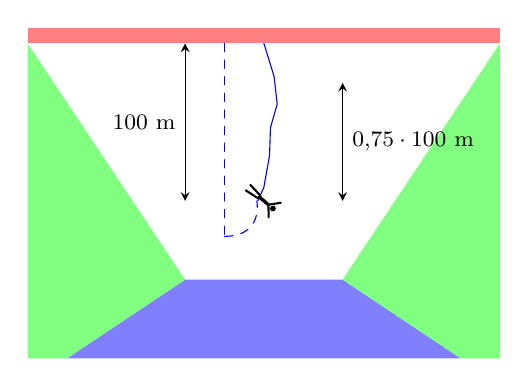
\begin{tikzpicture}[>=stealth,line join=round,line cap=round,font=\footnotesize,scale=1]
			\fill[blue!50] (-2.5,0)--(2.5,0)--(1,1)--(-1,1)--cycle;
			\fill[green!50]
			(-2.5,0)--(-3,0)--(-3,4)--(-1,1)--cycle
			(2.5,0)--(3,0)--(3,4)--(1,1)--cycle
			;
			%\draw[<->][dashed, line width=1.2] (0,4)--(0,2);
			\draw[blue, decorate,decoration=random steps ] (0,4) arc (25:-35:1 and 2);
			\draw [blue,dashed] (-.5,4)--(-.5,1.5);
			\draw[<->] (-1,4)--(-1,2)node[midway,left]{$100$ m};
			\draw[<->] (1,3.5)--(1,2)node[midway,right]{$0{,}75\cdot 100$ m};
			\fill[red!50] (-3,4) rectangle (3,4.2) ;
			\draw[blue, dashed] (-.5,1.55)..controls +(0:0.5) and +(-2:0)..(-.09,2) coordinate[pos=.5];
			\begin{scope}[line width=0.75pt,scale=0.15,rotate=-130,transform canvas={yshift=2cm}]
				\fill (0,1) circle (7pt);
				\draw 
				(0,0.5)--(0.8,1.2)
				(0,0.5)--(-0.8,1.2)
				;
				\draw[line width=1.2pt]
				(0,0.5)--(0,-0.5)
				;
				\draw 
				(-0.15,-0.5)--(0.15,-0.5)
				(-0.15,-0.5)--(-0.3,-1.75)
				(0.15,-0.5)--(0.3,-1.75)
				;
			\end{scope}
			%========================
	\end{tikzpicture}}
	\loigiai{
		Gọi $u_n$ là độ dài dây kéo sau $n$ lần rơi xuống $(n \in \mathbb{N})$.\\
		Ta có $u_0=100~(\mathrm{m})$.\\
		Sau lần rơi đầu tiên độ dài dây kéo còn lại là $u_1=100\cdot 75 \%~(\mathrm{m})$.\\
		Sau cú nhảy tiếp theo độ dài dây kéo còn lại là $u_2=100\cdot 75 \% \cdot 75 \%=100 \cdot (75 \%)^2~(\mathrm{m})$.\\
		$\ldots\ldots\ldots\ldots\ldots\ldots\ldots$\\
		Dãy số này lập thành một cấp số nhân có số hạng đầu là $100$ và công bội $q=0{,}75 \%$, có công thức tổng quát $u_n=100 \cdot(0{,}75 \%)^{n-1}~(\mathrm{m})$.\\
		Tổng quãng đường người đó đi được sau $10$ lần kéo lên và lại rơi xuống là
		$$
		S_{10}=\dfrac{100\left(1-(75 \%)^{10}\right)}{1-75 \%} \approx 377~(\mathrm{m}).
		$$}
\end{bt}

\begin{bt}%[1D2V3-8]
% nguon: Archive/2025-Sangtac/Khoi11/Data/1-KNTT/KNTT_1-OTHK1_De02.tex #4770

Một gia đình mua một chiếc ô tô giá $800$ triệu đồng. Trung bình sau mỗi năm sử dụng, giá trị còn lại của ô tô giảm đi $5\%$ (so với năm trước đó). Sau $10$ năm, giá trị của ô tô ước tính còn bao nhiêu triệu đồng? (kết quả làm tròn đến hàng triệu).

\shortans{479}
	\loigiai{
	Giả sử giá trị ban đầu của chiếc ô tô là $(u_0 = 800)$ triệu đồng. Sau mỗi năm sử dụng, giá trị còn lại của ô tô giảm đi $5\%$.\\
	Ta có thể tính giá trị của ô tô sau $n$ năm bằng công thức: $u_n = u_0 \cdot (1-5\%)^n$.\\
	Sau $10$ năm, giá trị ô tô là: $u_{10} = 800 \cdot (1-5\%)^{10} = 478{,}99$ (triệu đồng).\\
	Vậy sau $10$ năm giá trị ô tô là $479$ triệu đồng.
	}
\end{bt}

\begin{bt}%[1D2V2-7]
% nguon: Archive/2025-Sangtac/Khoi11/Data/1-KNTT/KNTT_1-OTGK1_De03.tex #4840
%[Dự án soạn đề kiểm tra Toán 11 GHKI NH24-25- Thanh Phong]%[KNTT_1-OTGK1-De03]
	\immini[thm]{Một chồng cột gỗ được xếp thành các lớp, hai lớp liên tiếp hơn kém nhau $1$ cột gỗ (Hình vẽ minh họa). Gọi $u_n$ là số cột gỗ nằm ở lớp thứ $n$ tính từ trên xuống và cho biết lớp trên cùng có $14$ cột gỗ. Hãy xác định số cột gỗ ở hàng thứ $20$?	
	}{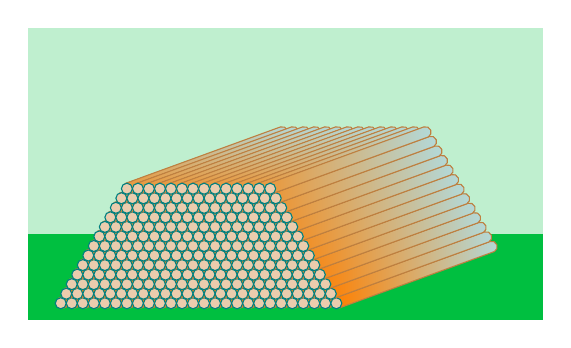
\begin{tikzpicture}[font=\footnotesize, line join=round, line cap=round, >=stealth,scale=0.35]
		\def\r{0.2}
		\def\n{25}
		\def\g{110}
		\fill[teal!50!green](-6*\r,-3*\r)rectangle(3.5*\n*\r,0.5*\n*\r);
		\fill[teal!50!green,opacity=0.25](3.5*\n*\r,3*\r)rectangle(-6*\r,2*\n*\r);
		\foreach \j in {0,...,12}{
			\pgfmathsetmacro{\m}{\n-\j}
			\foreach \i in{0,...,\m}{
				\fill[left color=orange, right color=teal!30,draw=brown](2*\i*\r,0)++(60:2*\j*\r)++(\g:\r)--++(\g-90:6)arc(\g:-60:\r)--++(\g-270:6)--cycle;
				\fill[orange!20!brown!40,draw=teal](2*\i*\r,0)++(60:2*\j*\r)circle(\r);
			}
		}
		\end{tikzpicture} }
	\shortans{33}
	\loigiai{
		\begin{itemize}
			\item Theo giả thiết ta có công thức truy hồi là $\heva{&u_1=14\\&u_{n+1}=u_n+1.}$
			\item Dùng phương pháp quy nạp toán học chứng minh được $u_n=13+n$.
			\item Khi đó hàng thứ $20$ sẽ có $u_{20}=13+20=33$ (cột gỗ).
		\end{itemize}
	}
\end{bt}

\begin{bt}%[1D2V3-8]
% nguon: Archive/2025-Sangtac/Khoi11/Data/1-KNTT/KNTT_1-OTGK1_De04.tex #4862
%[Dự án soạn đề kiểm tra Toán 11 GHKI NH24-25 - Nguyen Huynh]%[KNTT_1-OTGK1-De04]
	Người ta thiết kế một cái tháp gồm $11$ tầng theo cách: Diện tích bề mặt trên của mỗi tầng bằng nửa diện tích mặt trên của tầng ngay bên dưới và diện tích bề mặt trên của tầng 1 bằng nửa diện tích đế tháp. Biết diện tích đế tháp là $12\,288$ m$^2$, tính diện tích mặt trên cùng (đơn vị m$^2$).
	
	\shortans[]{6}
	\loigiai{
		Gọi $u_0$ là diện tích đế tháp và $u_n$ là diện tích bề mặt trên của tầng thứ $n$, với $1\le n\le 11$. Theo giả thiết, ta có $u_{n+1}=\dfrac{1}{2}u_n, 0\le n\le 10$. 
		Dãy số $(u_n)$ lập thành cấp số nhân với số hạng đầu $u_0=12288$ và công bội $q=\dfrac{1}{2}$.\\ 
		Diện tích mặt trên cùng của tháp là $$u_{11}=u_0\cdot q^{11}=12288. {\left(\dfrac{1}{2}\right)}^{11}=6\,\mathrm m^2.$$
	}
\end{bt}

\begin{bt}%[1D2V2-7]
% nguon: Archive/2025-Sangtac/Khoi11/Data/1-CTST/CTST_1-OTGK1_De08.tex #4870

Một kiến trúc sư thiết kế một hội trường với $15$ ghế ngồi ở hàng thứ nhất, $18$ ghế ngồi ở hàng thứ hai, $21$ ghế ngồi ở hàng thứ ba, và cứ như vậy (số ghế ở hàng sau nhiều hơn $3$ ghế so với số ghế ở hàng liền trước nó). Nếu muốn hội trường đó có sức chứa ít nhất $870$ ghế ngồi thì kiến trúc sư đó phải thiết kế tối thiểu bao nhiêu hàng ghế?
\shortans[0]{20}
\loigiai{
Số ghế ở mỗi hàng của nhà hát lập thành một cấp số cộng với số hạng đầu $u_1=15$ và công sai $d=3$. Gọi $n$ là số hàng ghế trong hội trường. \\
Tổng các số hạng này là
$S_{n}=\dfrac{n}{2}\left[2u_1+(n-1)d\right]=\dfrac{n}{2}\left[2\cdot 15+(n-1)\cdot 3\right]=\dfrac{n}{2}(3n+27)\ge 870$.\\
Do đó $3n^2+27n-1740\ge0$.\\
Giải bất phương trình bậc hai này ta được $n\le-29 \text{\ (loại)}$ và $n\ge 20$.\\
Vậy phải thiết kế tối thiểu $20$ hàng ghế.
}
\end{bt}

\begin{bt}%[1D2V3-8]
% nguon: Archive/2025-Sangtac/Khoi11/Data/1-CTST/CTST_1-OTGK1_De08.tex #4871

Một công ty xây dựng mua một chiếc máy ủi với giá $3$ tỉ đồng. Cứ sau mỗi năm sử dụng, giá trị của chiếc máy ủi này lại giảm $20 \%$ so với giá trị của nó trong năm liền trước đó. Giá trị còn lại của chiếc máy ủi đó sau $5$ năm sử dụng là bao nhiêu triệu đồng?
\shortans[0]{480}
\loigiai{
Gọi $(u_n)$ là dãy số biểu diễn giá trị của chiếc máy ủi theo từng năm. \\
Dãy số này là một cấp số nhân có $u_1=3$, $q=0{,}2$.\\
Số hạng tổng quát của cấp số nhân này là $u_n=3\cdot 0{,}2^{n-1}$.\\
Ta có $u_5=3\cdot 0{,}2^4=\dfrac{3}{325}=4{,}8\cdot10^{-3}$.\\
Tương ứng giá trị của chiếc máy ủi sau $5$ năm là $480$ triệu đồng.
}
\end{bt}

\begin{bt}%[1D2V3-8]
% nguon: Archive/2025-Sangtac/Khoi11/Data/1-CTST/CTST_1-OTHK1_De02.tex #4900

Một du khách vào chuồng đua ngựa đặt cược, lần đầu đặt $50\,000$ đồng, mỗi lần sau đặt gấp đôi lần cọc trước. Người đó thua $10$ lần liên tiếp và thắng ở lần thứ $11$. Hỏi du khách trên thắng hay thua bao nhiêu tiền (đơn vị nghìn đồng)?
\shortans[6]{$50$}
\loigiai{
Số lần đặt cược tạo thành một cấp số nhân với số hạng đầu $u_1=50\,000$ và công bội $q=2$.\\
Du khách thua trong $10$ lần liên tiếp nên tổng số tiền thua là
$${S_{10}}=u_1+u_2+\cdots+{u_{10}}=u_1\cdot\dfrac{1-{q^{10}}}{1-q}=50\,000\cdot\dfrac{1-2^{10}}{1-2}=51\,150\,000.$$
Số tiền du khách thắng trong lần thứ $11$ là $u_{11}=u_1\cdot q^{10}=50000\cdot2^{10}=51\,200\,000$.\\
Ta có $u_{11}-S_{10}=51200000-51150000=50\,000$ nên du khách đó thắng $50\,000$ đồng.
}
\end{bt}

\begin{bt}%[1D2V2-7]
% nguon: Archive/2025-Sangtac/Khoi11/Data/1-CTST/CTST_1-OTHK1_De03.tex #4909

	Người ta thiết kế số ghế ngồi trên khán đài một sân vận động bóng đá như sau. Hàng ghế đầu tiên gần sân bóng đá nhất có $1600$ ghế. Kể từ hàng thứ hai trở đi, mỗi hàng liền sau hơn hàng liền trước 400 ghế. Muốn sức chứa trên khán đài có ít nhất $222000$ ghế thì cần phải thiết kế ít nhất bao nhiêu hàng ghế?
		\shortans[0]{$150$}	
	\loigiai{
		Gọi $n$ là số hàng ghế cần thiết kế và $u_1$ số ghế ở hàng đầu tiên\\
		Theo đề ta có $u_1=1600$, $u_2=u_1+400$ và $S_n\ge 222000\Leftrightarrow n.u_1+\dfrac{n.\left(n-1\right)d}{2}\ge 222000$\\
		$\Leftrightarrow 1600n+\dfrac{n\left(n-1\right)400}{2}\ge 222000\Leftrightarrow n^2+2800-444000 \ge 0 \Leftrightarrow n\ge 150,24$.\\
		Vậy suy ra cần thiết kế ít nhất $150$ hàng ghế.}
\end{bt}

\begin{bt}%[1D2V2-7]
% nguon: Archive/2025-Sangtac/Khoi11/Data/1-CTST/CTST_1-OTHK1_De01.tex #4919

Một gia đình cần khoan một cái giếng để lấy nước. Họ thuê một đội khoan giếng đến để khoan giếng nước. Biết giá của một mét khoan đầu tiên là $75\,000$ nghìn đồng, kể từ mét khoan thứ hai giá mỗi mét khoan tăng lên $6\,000$ nghìn đồng so với giá của mét khoan trước đó. Biết cần phải khoang sâu $80\mathrm{\,m}$ thì mới có nước. Vậy gia đình cần phải trả bao nhiêu tiền để khoan cái giếng đó? (kết quả làm tròn đến hàng đơn vị của triệu đồng).
\shortans[6]{$25$}
\loigiai{
Giá tiền khoan mỗi mét giếng (bắt đầu từ mét đầu tiên) lập thành cấp số cộng $(u_n)$ có số hạng đầu $u_1=75\,000$ và công sai $d=6\,000$.\\
Do cần khoan $80\mathrm{\,m}$ nên tổng số tiền cần trả là\\ $$S_{80}=u_1+u_2+\ldots+u_{80}=\dfrac{80}{2}\left(2\cdot 75\,000+79\cdot 6\,000 \right)=24\,960\,000\approx 25\,\text{(triệu đồng)}.$$
}
\end{bt}

\begin{bt}%[1D2V3-8]
% nguon: Archive/2025-Sangtac/Khoi11/Data/1-CTST/CTST_1-OTHK1_De01.tex #4920

Bạn Lan thả một quả bóng cao su từ độ cao $12\mathrm{\,m}$ theo phương thẳng đứng. Mỗi khi chạm đất nó lại nảy lên theo phương thẳng đứng với độ cao bằng $\dfrac{2}{3}$ độ cao trước đó. Tính tổng quãng đường quả bóng đi được cho đến khi quả bóng dừng hẳn.
\shortans[6]{$60$}
\loigiai{
Các quãng đường khi bóng đi xuống tạo thành một cấp số nhân lùi vô hạn với số hạng đầu $u_1=12$ và công bội $q=\dfrac{2}{3}$.\\
Do đó tổng quảng đường mà quả bóng đi xuống là $S=\dfrac{u_1}{1-q}=\dfrac{12}{1-\dfrac{2}{3}}=36\mathrm{\,m}$.\\
Tổng quãng đường của quả bóng đi được cả lên và xuống đến khi quả bóng dừng hẳn là $$2S-12=2\cdot 36-12=60\mathrm{\,m}.$$
}
\end{bt}

\begin{bt}%[1D2V3-8]
% nguon: Archive/2025-Sangtac/Khoi11/Data/1-CTST/CTST_1-OTHK1_De05.tex #4949
%[Câu 18]
	Vào đầu mỗi tháng, ông An đều gửi vào ngân hàng số tiền cố định $30$ triệu đồng theo hình thức lãi kép với lãi suất $0{,}6\%$ mỗi tháng. Tính số tiền ông An có được sau tháng sau tháng thứ hai
	\shortans[0]{$60{,}5$}
	\loigiai{
		Số tiền ông An có được:\\
		$\bullet$ Sau tháng thứ nhất là $T_1=30+30 \cdot \dfrac{0{,}6}{100}=30{,}18$ (triệu đồng).\\
		$\bullet$ Sau tháng thứ hai là $T_2=30+30 \left(1+\dfrac{0{,}6}{100}\right)+\left[30+30\left(1+\dfrac{0{,}6}{100}\right)\right]\dfrac{0{,}6}{100} \approx 60{,}54$ (triệu đồng).
	}
\end{bt}

\begin{bt}%[1D2V3-8]
% nguon: Archive/2025-Sangtac/Khoi11/Data/1-CTST/CTST_1-OTHK1_De05.tex #4950
%[Câu 19]
	Chu kì bán rã của nguyên tố phóng xạ polonium $210$ là $138$ ngày (nghĩa là sau $138$ ngày khối lượng của nguyên tố đó chỉ còn một nửa). Biết khối lượng còn lại của $20$ gam polonium $210$ sau $7314$
	ngày (khoảng $20$ năm) có dạng $4{,}44 \cdot 10^{-a}$ với $a$ là số nguyên. Tính giá trị của biểu thức $P=a^2$.
	\shortans[0]{225}
	\loigiai{
		Gọi $u_n$ (gam) là khối lượng còn lại của $20$ gam polonium $210$ sau $n$ chu kì bán rã.\\
		Ta có $7\,314$ ngày gồm $53$ chu kì bán rã ($1$ chu kì hết $138$ ngày). Theo đề bài ra, ta cần tính $u_{53}$.\\
		Từ giả thiết suy ra dãy $(u_n)$ là một cấp số nhân với số hạng đầu là $u_1=20$ và công bội $q=0{,}5$.\\
		Suy ra $u_n=20 \cdot(0{,}5)^{n-1}$.\\
		Do đó $u_{53}=20 \cdot(0{,}5)^{52} \approx 4{,}44 \cdot 10^{-15}$. 
	}
\end{bt}

\begin{bt}%[1D2V3-8]
% nguon: Archive/2025-Sangtac/Khoi11/Data/1-CTST/CTST_1-OTGK1_De06.tex #4998

Tỉ lệ tăng dân số mỗi năm của một tỉnh A từ năm $2010$ đến năm $2019$ là $0{,}4\%$. Vì thực hiện chính sách về dân số nên tỉnh A dự kiến từ năm $2020$ đến $2035$ tỉ lệ tăng dân số mỗi năm chỉ còn lại $0{,}35\%$. Theo thống kê số dân tỉnh A năm $2021$ nhiều hơn năm $2017$ là $40\,500$ người. Ước tính số dân tỉnh A vào năm $2035$ (làm tròn đến hàng nghìn) là $\overline{abcd000}$. Hỏi $\overline{abcd}$ bằng bao nhiêu?
\shortans[]{$2862$}
\loigiai{
Gọi dân số tỉnh A năm $2010$ là $a$ (người, $a \in \mathbb{N}^*$).\\
Số dân mỗi năm của tỉnh A từ năm $2010$ đến $2019$ là một cấp số nhân $\left(u_n\right)$ với số hạng đầu $u_1=a$ và công bội $q=1+0{,}4\%=1{,}004$.\\
Số dân tỉnh A năm $2017$ là $u_8=u_1 \cdot q^7=a \cdot 1{,}004^7$.\\
Số dân tỉnh A năm $2019$ là $u_{10}=u_1 \cdot q^9=a \cdot 1{,}004^9$.\\
Số dân tỉnh A năm $2020$ là $a \cdot 1{,}004^9 \cdot 1{,}0035$.\\
Số dân mỗi năm của tỉnh A từ năm $2020$ đến $2035$ là một cấp số nhân $\left(v_n\right)$ với số hạng đầu $v_1=a \cdot 1{,}004^9 \cdot 1{,}0035$ và công bội $q'=1+0{,}35 \%=1{,}0035$.\\
Số dân của tỉnh A năm $2021$ là $a \cdot 1{,}004^9 \cdot 1{,}0035^2$.\\
Vì số dân tỉnh A năm $2021$ nhiều hơn năm $2017$ là $40500$ người nên ta có
\[
a \cdot 1{,}004^9 \cdot 1{,}0035^2-a \cdot 1{,}004^7=40\;500 \Rightarrow a \approx 2\,610\,894.
\]
Số dân tỉnh A năm $2035$ là $2\,610\,894\cdot 1{,}004^9 \cdot 1{,}0035^{16} \approx 2\,862\,000$ người.\\
Vậy $\overline{abcd}=2\,862$.
	}
\end{bt}

\begin{bt}%[1D2V3-8]
% nguon: Archive/2025-Sangtac/Khoi11/Data/1-CTST/CTST_1-OTGK1_De05.tex #5007
%[Câu 4]
	Tỉnh Trà Vinh năm $2022$ có dân số là $1\,019\,258$ người và tốc độ gia tăng dân số trung bình mỗi năm là $0{,}06$ \%. Dự đoán dân số của tỉnh Trà Vinh năm $2030$ là bao nhiêu (Làm tròn kết quả đến hàng phần nghìn)?
	\shortans{$1024$}
	\loigiai{
		Đây là cấp số nhân với $u_1 = 1\,019\,258$, công bội $q=1{,}06$. \\
		Năm $2030$ là năm thứ $9$, tức là dân số tỉnh Trà Vinh năm $2030$ dự đoán là\\ \centerline{$u_9 = u_1\cdot q^{9-1} = 1\,019\,258 \cdot \left(1+\dfrac{0{,}06}{100}\right)^{8} = 1\,024\,160{,}725\approx 1\,024$ nghìn người.}
	}
\end{bt}

\begin{bt}%[1D2V3-8]
% nguon: Archive/2025-Sangtac/Khoi12/Data/1-KNTT/KNTT_1-OTGK1_De08.tex #5045

	Một du khách đặt cược đua ngựa online, lần đầu đặt $50\,000$ đồng, mỗi lần sau số tiền đặt gấp đôi lần tiền đặt cọc trước. Người đó thua $9$ lần liên tiếp và thắng ở lần thứ $10$. Hỏi du khách lãi bao nhiêu tiền? (Đơn vị: nghìn đồng) 
	
	\shortans{50}
	\loigiai{
		Theo giả thiết, số tiền du khách đặt trong mỗi lần đặt cược lập thành một cấp số nhân với $u_1=50\,000$ và công bội $q=2$.\\
		Du khách thua trong $9$ lần đầu tiên nên tổng số tiền thua là $$S_9=u_1+u_2+..+u_9=\dfrac{u_1\left(1-q^9\right)}{1-q}=\dfrac{50\,000\left(1-2^9\right)}{1-2}=25\,550\,000 \text{ đồng}.$$
		Số tiền mà du khách thắng trong lần thứ $10$ là $u_{10}=u_1\cdot q^9=50\,000\left(2\right)^9=25\,600\,000$ đồng.\\
		Ta có $u_{10}-S_9=50\,000>0$ nên du khách lãi được $50\,000$ đồng.}
\end{bt}

\begin{bt}%[1D2V2-7]
% nguon: Archive/2025-Sangtac/Khoi12/Data/1-KNTT/KNTT_1-OTGK1_De07.tex #5060

	Nếu anh Nam nhận được lời mời làm việc cho một công ty nước ngoài với mức lương khởi điểm là $35000$ đô la mỗi năm và được tăng thêm $1400$ đô la lương mỗi năm, thì sẽ mất bao nhiêu năm làm việc để tổng lương mà anh Nam nhận được là $319200$ đô la?
	
	\shortans{8}
	\loigiai{
		Gọi $u_n$ là lương anh Nam nhận được ở năm thứ $n$.\\
		Ta có lương khởi điểm là $35000$ đô la mỗi năm nên $u_1 = 35000;  d = 1400$.\\
		Mỗi năm lương được tăng thêm $1400$ đô la nên $u_n = u_{n-1} + 1400, n \geq 2, n \in \mathbb{N^*}$.\\
		Như vậy dãy số tiền lương của anh Nam nhận được qua các năm là $u_1;u_2;u_3;...;u_n$ là một
		cấp số cộng có $u_1 = 35000; d = 1400$.\\
		Áp dụng công thức tính tổng $n$ số hạng đầu của cấp số cộng với
		$S_n = 319200; u_1 = 35000; d = 1400$
		ta có\\
		$319200 = S_n = \dfrac{n(2u_1+(n-1)\cdot 1400)}{2}
		\Leftrightarrow 
		n = 8.$\\
		Vậy sau $8$ năm làm việc thì tổng lương mà anh Nam nhận được là $319200$ đô la.}
\end{bt}

\begin{bt}%[1D2C2-7]
% nguon: Archive/2025-Sangtac/Khoi12/Data/1-CTST/CTST-1-OTGK1-De07.tex #5072

	Khi kí kết hợp đồng với người lao động, một doanh nghiệp đề xuất hai phương án trả lương như sau:\\
	\textit{Phương án 1}: Năm thứ nhất, tiền lương là $120$ triệu đồng. Kể từ năm thứ hai trở đi, mỗi năm tiền lương được tăng $18$ triệu đồng.\\
	\textit{Phương án 2}: Quý thứ nhất, tiền lương là $24$ triệu đồng. Kể từ quý thứ hai trở đi, mỗi quý tiền lương được tăng $1{,}8$ triệu đồng.\\
	Tìm $n$ (với $n \in \mathbb{N^*}$) để từ năm thứ $n$ trở đi thì tổng số tiền lương nhận được trong $n$ năm đi làm ở phương án thứ hai nhiều hơn ở phương án thứ nhất?
	\shortans{$4$}
	\loigiai{
		\begin{itemize}
			\item \textit{Phương án 1}: $u_1=120$ và $d=18$, đơn vị: triệu đồng.
			\item \textit{Phương án 2}: 1 quý $=$ 3 tháng, $u_1=24$ và $d=1{,}8$ đơn vị: triệu đồng.
		\end{itemize}
		Gọi lần lượt $S_n$ và $Q_n$ là tổng tiền lương sau $n$ năm của phương án 1 và phương án 2. Ta có\\
		$S_n=\dfrac{(u_1+u_n) \cdot n}{2}=\dfrac{[120+120+(n-1) \cdot 18] \cdot n}{2}$.\\
		$Q_n=\dfrac{(u_1+u_n) \cdot n}{2}=\dfrac{[24+24+(4n-1) \cdot 1{,}8] \cdot 4n}{2}$ (vì 1 năm có 4 quý).\\
		Ta có:
		\begin{eqnarray*}
			&Q_n>S_n&\Leftrightarrow \dfrac{[48+(4n-1) \cdot 1{,}8] \cdot 4n}{2}>\dfrac{[240+(n-1) \cdot 18] \cdot n}{2}\\
			&&\Leftrightarrow \left[ 48+\dfrac{36}{5}n-\dfrac{9}{5}\right]2n>\dfrac{(240+18n-18)n}{2}\\
			&&\Leftrightarrow \dfrac{72}{5}n^2+\dfrac{462}{5}n>9n^2+111n\\
			&&\Leftrightarrow n<0 \text{ hoặc } n>\dfrac{31}{9}
		\end{eqnarray*}
		Vì $n>0$ nên $n>3{,}4$. Vậy từ năm thứ $4$ trở đi $Q_n>S_n$.
	}
\end{bt}

\begin{bt}%[1D2V3-8]
% nguon: Archive/2025-Sangtac/SP-Main/Data/1-KNTT/KNTT_1-OTHK1_De01.tex #5079

Theo báo cáo của Chính phủ, dân số của nước ta tính đến tháng 12 năm 2018 là $95{,}93$ triệu người, nếu tỉ lệ tăng trưởng dân số trung bình hằng năm là  $1{,}33\%$ thì dân số nước ta vào tháng 12 năm 2025 là bao nhiêu? (kết quả làm tròn đến hàng triệu).
	\shortans[0]{$105$}
	\loigiai{
	Theo tỉ lệ tăng trưởng dân số trung bình hằng năm là $1{,}33\%$  thì ta có:\\
	$-$ Tháng 12 năm 2019, dân số nước ta là \\
$u_1=95{,}93 + 95{,}93\cdot 1{,}33\%= 95{,}93\left(1 + 0{,}0133\right) =95{,}93\cdot 1{,}0133$.\\
	$-$ Tháng 12 năm 2020, dân số nước ta là \\
	$u_2=(95{,}93\cdot 1{,}0133) + (95{,}93\cdot 1{,}0133)\cdot 0{,}0133 =95{,}93\cdot 1{,}0133\%= 95{,}93\cdot 1{,}0133^2$.\\
	$-$ Tương tự ta có, tháng 12 năm 2021, dân số nước ta là $u_3=95{,}93\cdot 1{,}0133^3$.\\
	$-$ Theo quy luật đó, ta biết dân số nước ta vào tháng 12 năm thứ $n$  kể từ năm 2019 là $u_n= 95{,}93\cdot 1{,}0133^n$ với $n$ nguyên dương, $n \ge 1$.\\
	$-$ Vậy Tháng 12 năm 2025, dân số nước ta là $u_7= 95{,}93\cdot 1{,}0133^7 \approx 105$ triệu người.
	}
\end{bt}

\begin{bt}%[1D2V3-8]
% nguon: Archive/2025-Sangtac/SP-Main/Data/1-KNTT/KNTT_1-OTHK1_De10.tex #5085

	Giả sử một thành phố có dân số năm 2022 là khoảng $2{,}1$ triệu người và trong những năm tiếp theo, cứ năm sau dân số lại tăng thêm $0{,}75 \%$ so với năm trước đó. Nếu tốc độ gia tăng dân số vẫn giữ nguyên như trên thì uớc tính vào năm nào dân số của thành phố đó sẽ khoảng $2\,262\,923$ người?
	\shortans[0]{$2032$}
	\loigiai{
		\begin{itemize}
		\item Dân số năm 2022 là $u_0=2{,}1\cdot 10^6$.
		\item Dân số sau 1 năm (tức năm 2023) là $u_1=u_0+u_0 \cdot 0{,}075=u_0 \cdot 1{,}0075$.
		\item Dân số sau 2 năm (tức năm 2024) là $u_2=u_1+u_1 \cdot 0,0075=u_0 \cdot 1{,}0075^2$.
		\item \ldots
		\item Dân số sau $n$ năm là $u_n=u_0 \cdot 1{,}0075^n=2{,}1 \cdot 10^6 \cdot 1{,}0075^n$.
		\end{itemize}
		Khi đó $u_n=2\,262\,923 \Leftrightarrow 2{,}1 \cdot 10^6 \cdot 1{,}0075^n=2\,262\,923 \Leftrightarrow n \simeq 10$. \\
		Vậy vào năm $2022+10=2032$ thì dân số thành phố đó sẽ khoảng $2\,262\,923$ người.
}
\end{bt}

\begin{bt}%[1D2V3-7]
% nguon: Archive/2025-Sangtac/SP-Main/Data/1-KNTT/KNTT_1-OTGK1_De02.tex #5095

	Quốc gia $X$ có trữ lượng dầu mỏ là $120$ triệu thùng vào đầu năm $2022$. Theo dự báo với mức khai thác dầu không đổi như năm $2022$ thì trữ lượng dầu của nước này sẽ hết sau đúng $50$ năm nữa. Do nhu cầu phát triển kinh tế, kể từ năm $2023$ trở đi mức khai thác dầu mỏ mỗi năm của quốc gia $X$ tăng lên $5 \%$ so với năm trước. Hỏi đến hết năm $2035$ thì trữ lượng dầu của nước này còn lại bao nhiêu thùng (làm tròn đến hàng đơn vị)?
	\shortans[0]{$73$}
	\loigiai{
	Trữ lượng dầu mỏ khai thác trong năm $2022$ là $\dfrac{120}{50}=\dfrac{12}{5}$ triệu thùng.\\
	Trữ lượng khai thác dầu mỏ hàng năm tính từ năm $2022$ đến năm $2035$ là
	$$\dfrac{12}{5}; \dfrac{12}{5}\cdot 1{,}05;\dfrac{12}{5}\cdot \left(1{,}05\right)^2;\dfrac{12}{5}\cdot \left(1{,}05\right)^3;\cdots;\dfrac{12}{5}\cdot \left(1{,}05\right)^{13}.$$
	Dãy trên là một cấp số nhân có $u_1=\dfrac{12}{5}$, công bội $q=1{,}05$.\\
	Tổng trữ lượng dầu khai thác từ năm $2022$ đến năm $2035$ là
	$$S_{14}=u_1\cdot \dfrac{1-q^{14}}{1-q}=\dfrac{12}{5}\cdot \dfrac{1-\left(1{,}05\right)^{14}}{1-1{,}05}\approx 47 \text{ (triệu thùng).}$$
	Vậy tính đến hết năm $2035$ thì trữ lượng dầu của nước này còn lại $120-47=73$ triệu thùng.
	}
\end{bt}

\begin{bt}%[1D2V3-8]
% nguon: Archive/2025-Sangtac/SP-Main/Data/1-KNTT/KNTT_1-OTGK1_De06.tex #5101
%[2025-K11-SangtacdeGKI]%[ChuongtrinhKNTT, Trần Lê Tuấn Anh]
	Ông Năm vay mượn ngân hàng $200$ triệu đồng với lãi suất $6\%$/năm. Ông đồng ý trả theo kì hạn $5$ triệu đồng mỗi tháng. Hỏi số tiền mà ông Năm còn nợ ngân hàng sau $1$ năm nhiều hơn so với số tiền ông Năm còn nợ ngân hàng sau $3$ năm là bao nhiêu triệu đồng (làm tròn đến hàng đơn vị)? Biết công thức tính số tiền nợ còn lại sau thời gian $n$ là $u_n=N(r+1)^n-\dfrac{A}{r}[(r+1)^n-1]$, với $N$ là số tiền nợ ban đầu, $r$ là lãi suất theo chu kì, $n$ là thời gian trả nợ theo đơn vị của lãi suất, $A$ là số tiền trả nợ theo kì hạn.
	\shortans[0]{$108$}
	\loigiai{
		Lãi suất $r=6\%$/năm $=0,5\%$/tháng.\\
		Số tiền ông Năm nợ ban đầu là $N=200$ triệu đồng.\\
		Số tiền trả theo kì hạn là $A=5$ triệu đồng.\\
		Thời gian trả nợ của ông Năm là $n$ (tháng).\\
		Số tiền ông Năm còn nợ sau $n$ tháng là\\ $u_n=200(0{,}5\%+1)^n=\dfrac{5}{0{,}5\%}[(0{,}5\%+1)^n-1]$.\\
		Số tiền ông Năm còn nợ sau $12$ tháng ($1$ năm) là \\
		${{u}_{12}}=200{{\left( 0{,}5\%+1 \right)}^{12}}-\dfrac{5}{0{,}5\%}\left[ {{\left( 0{,}5\%+1 \right)}^{12}}-1 \right]\approx 151$ (triệu đồng).\\
		Số tiền ông Năm còn nợ sau $36$ tháng ($3$ năm) là \\
		${{u}_{36}}=200{{\left( 0{,}5\%+1 \right)}^{36}}-\dfrac{5}{0{,}5\%}\left[ {{\left( 0{,}5\%+1 \right)}^{36}}-1 \right]\approx 43$ (triệu đồng).\\
		Số tiền mà ông Năm còn nợ ngân hàng sau $1$ năm nhiều hơn so với số tiền ông Năm còn nợ ngân hàng sau $3$ năm là $151-43=108$ triệu đồng.
	}
\end{bt}

\begin{bt}%[1D2V3-8]
% nguon: Archive/2025-Sangtac/SP-Main/Data/1-KNTT/KNTT_1-OTGK1_De06.tex #5103
%[2025-K11-SangtacdeGKI]%[ChuongtrinhKNTT, Trần Lê Tuấn Anh]
	Vào năm $2023$, dân số của Philippines là $118\,223\,042$ người và tốc độ tăng trưởng dân số là $1{,}5\%$. Nếu tốc độ tăng trưởng dân số này được giữ nguyên hằng năm, hãy ước tính dân số của Philippines vào năm $2030$ là bao nhiêu triệu người (làm tròn đến hàng đơn vị). (Nguồn: https://danso.org/philippines/).
	\shortans[0]{$131$}
	\loigiai{
		Đây là bài toán cấp số nhân.\\
		Giả sử dân số của Philippines là N. Vì tốc độ tăng trưởng dân số là $1{,}5\%$ nên sau một năm, số dân tăng thêm là $1{,}5\% \cdot N$.\\
		Vậy dân số của Philippines vào năm sau là $N + 1{,}5\% \cdot N = 101{,}5\% \cdot N = 1{,}015N$.\\
		Như vậy, dân số của Philippines sau mỗi năm lập thành một cấp số nhân với số hạng đầu $u_1 = N$ và công bội $q = 1{,}015$.\\
		Theo bài ra ta có $u_1 = 118\,223\,042$ ứng với năm $2023$.\\
		Ta có $2030-2023 = 7$.\\
		Dân số của Philippines vào năm $2030$ chính là dân số của quốc gia sau $7$ năm kể từ năm $2023$, ứng với $u_8$ và ${{u}_{8}}={{u}_{1}}\cdot{{q}^{8-1}}=118\,223\,042\cdot{{\left( 1{,}015 \right)}^{8-1}}\approx 131\,209\,242$ (người) hay $131$ (triệu người).
	}
\end{bt}

\begin{bt}%[1D2V2-7]
% nguon: Archive/2025-Sangtac/SP-Main/Data/1-KNTT/KNTT_1-OTGK1_De04.tex #5108
%[Dự án soạn đề kiểm tra Toán 11 GHKI NH24-25 - Nguyen Huynh]%[KNTT_1-OTGK1-De04]
	Bác Bình muốn trồng cây cà phê trên một ngọn đồi như sau: Từ trên đỉnh đồi trồng hàng thứ nhất $2$ cây; đi xuống hàng thứ hai $5$ cây; đi xuống hàng thứ ba $8$ cây; $\ldots$; đi xuống hàng cuối cùng dưới chân đồi trồng $26$ cây. Theo cách trồng như trên bác bình trồng được bao nhiêu cây cà phê?
	\shortans[0]{126}
	\loigiai{
		Gọi $u_1;u_2;u_3; \ldots; u_n$ lần lượt là số cây hàng thứ nhất; hàng thứ hai; hàng thứ ba; \ldots; hàng thứ $n$.
		Ta có $u_1=2; u_2=5 \Rightarrow d=3$.\\
		Theo cách trồng của bác Bình số cây mỗi hàng lập thành một cấp số cộng với số hạng đầu $u_1=2$ và công sai $d=3$. Thật vậy, ta có
		\begin{itemize}
			\item $u_1= 2$ cây.
			\item $u_2=u_1+d = 2+3=5$ cây.
			\item $u_3=u_1+2d=5+3=8$ cây.
			\item \ldots
			\item $u_n = u_1+(n-1)d = 26$ cây.
		\end{itemize}
		Suy ra $2+(n-1)\cdot 3 =26 \Leftrightarrow n = 9$. Vậy có $9$ hàng cây.\\
		Do đó, số cây cà phê bác Bình trồng được là
		\[S_9 =\dfrac{9(2+26)}{2}=126 \text{ cây.} \]
	}
\end{bt}

\begin{bt}%[1D2V3-8]
% nguon: Archive/2025-Sangtac/SP-Main/Data/1-KNTT/KNTT_1-OTGK1_De04.tex #5109
%[Dự án soạn đề kiểm tra Toán 11 GHKI NH24-25 - Nguyen Huynh]%[KNTT_1-OTGK1-De04]
	Người ta thiết kế một cái tháp gồm $11$ tầng theo cách: Diện tích bề mặt trên của mỗi tầng bằng nửa diện tích mặt trên của tầng ngay bên dưới và diện tích bề mặt trên của tầng 1 bằng nửa diện tích đế tháp. Biết diện tích đế tháp là $12\,288$ m$^2$, tính diện tích mặt trên cùng (đơn vị m$^2$).
	\shortans[0]{$6$}
	\loigiai{
		Gọi $u_0$ là diện tích đế tháp và $u_n$ là diện tích bề mặt trên của tầng thứ $n$, với $1\le n\le 11$. Theo giả thiết, ta có $u_{n+1}=\dfrac{1}{2}u_n, 0\le n\le 10$. 
		Dãy số $(u_n)$ lập thành cấp số nhân với số hạng đầu $u_0=12288$ và công bội $q=\dfrac{1}{2}$.\\ 
		Diện tích mặt trên cùng của tháp là $$u_{11}=u_0\cdot q^{11}=12288. {\left(\dfrac{1}{2}\right)}^{11}=6\,\mathrm m^2.$$
	}
\end{bt}
